\documentclass[11pt, english, fleqn, DIV=15, headinclude, BCOR=2cm]{scrreprt}

\usepackage[
    color,
    bibatend,
]{../../header}

\graphicspath{{./}{../Figures/}}

\newcommand\MZ{M_{\mathrm Z^0}}
\newcommand\electron{\mathrm e^-}
\newcommand\positron{\mathrm e^+}

\usepackage{needspace}

\usepackage{mathtools}
\usepackage{listings}

\lstset{
    basicstyle=\small\ttfamily,
}

\hypersetup{
    pdftitle=
}

\usepackage{longtable}
\usepackage{subcaption}

\usepackage[all]{nowidow}

\subject{Lab report}
\title{Analysis of $Z_0$ decays}
\subtitle{Experiment E213 -- Universität Bonn}
\author{%
    Martin Ueding \\
    \small{\href{mailto:mu@martin-ueding.de}{mu@martin-ueding.de}}
    \and
    Lino Lemmer \\
    \small{\href{mailto:l2@uni-bonn.de}{l2@uni-bonn.de}}
}

\date{2016-03-02}

\publishers{Tutor: David Hohn}

\begin{document}

\maketitle

\begin{abstract}
    In this experiment we analyse data from electron positron collisions
    collected with the \textsc{opal} detector at the \textsc{lep} collider.
    Aim of the experiment is to have an insight in methods of data analysis in
    high energy physics.
    
    In the first part we learn to distinguish between the different decay
    channels of the $\mathrm{Z}^0$ boson by their signature in the detector
    with a small data sample.

    In the second part we want to find mass, decay width and partial cross
    section of the $\mathrm{Z}^0$ for different decay channels and the weak
    mixing angle angle from the forward backward asymmetry of the
    $\electron\positron \to \muup^-\muup^+$ reaction. We also want to verify
    the lepton universality and identify the number of neutrino generations.
    For this part we use preselected data and Monte Carlo events as help.
\end{abstract}

\tableofcontents

\chapter*{Permission to upload}

I, Martin Ueding, would like to scan and upload this lab report with your
corrections to my website \href{http://martin-ueding.de}{martin-ueding.de}.
There, the original lab report as well as the reviewed one will be licensed
under the “\href{http://creativecommons.org/licenses/by-sa/4.0/}{Creative
Commons Attribution-ShareAlike 4.0 International License}”. Is that okay with
you?

Yes $\Box$ \hspace{2cm} No $\Box$

\chapter{Theory}

\section{The standard model of particle physics}

In the standard model there are generally two types of elementary particles,
fermions with spin $s = 1/2$ and bosons with spin $s = 1$. Within the fermions
there are particles which exist freely (leptons) and ones which only exist in
bound states with each other (quarks). The latter make up heavier particles
(hadrons) like the two quarks particles called mesons and baryons consisting
from three quarks. 

The leptons are three generations of particles. In every
generation one can find one charged particle with $q = -e$. These are the
electron $\mathrm e^-$, the muon $\muup^-$ and the tauon $\tauup^-$. To each
one of them there belongs a very light uncharged neutrino
$\nuup_{\mathrm{e}/\muup/\tauup}$.

Within the quarks one also can find three generations. The first generation
containes the up quark u and the down quark d. In the second one there are
charm c and strange s and in the third one one can find the top and the bottom
quark. All quarks carry charge and mass.

All these particles interact through different interaction types, gravity,
electromagnetic interaction, weak interaction and strong interaction. The first
one plays no role in particle physics. The strong interaction acts only on the
quarks and is intermediated by gluons, the first type of bosons. The
electromagnetic interaction acts only on charged particles and the weak
interaction on all fermions. 

The electroweak interaction is a combination of the latter two interaction
types. Speaking of symmetries we combine the $\mathrm{SU}(2)$ symmetry of the
weak interaction with its three interaction particles $\mathrm W^0$, $\mathrm
W^1$ and $\mathrm W^2$ with the $\mathrm U(1)$ symmetry of the electromagnetic
interaction with its particle $\mathrm B^0$ to get two charged bosons $\mathrm
W^\pm$ and two uncharged ones, $\gammaup$ and $\mathrm Z^0$, which are
superpositions of $\mathrm W^0$ and $\mathrm B^0$. The angle between the
$\gammaup$ and the $\mathrm Z^0$ in the $\mathrm W^0$-$\mathrm B^0$ plane is
called weak mixing angle. Sometimes this is also called \enquote{Weinberg
angle}, but although Weinberg did many things, this angle was introduced by
somebody else.

\section{Interaction of particles with matter}

\subsection{Photons}

At different photon energies different interactions are dominant. At high
energy the pair production is the most likely process. For
this the photon needs an energy equal to the rest mass of the
particle-antiparticle pair or higher. Below this energy Compton scattering and
the photo effect are dominant. In these processes the photons lose their
energy to electrons or other particles and are very important for particle
detection in scintillators.

\subsection{Charged particles}

From all processes charged particles can undergo, like inelastic scattering
with orbiting electrons, elastic scattering with the nucleus, or energy
loss due to Cherenkov radiation or bremsstrahlung, the last is the most
important for our case. Bremsstrahlung occurs when a charged particle gets
accelerated in an Coulomb potential. The energy loss is highly dependent on
the particle's mass:
\[
        \od Ex \propto \frac 1{m^2}.
\]
This is the reason why this effect is most relevant for the light electrons
rather than for the heavier myons.

\section{Decay channels of the $\mathrm Z^0$ boson}

Since the $\mathrm Z^0$ doesn't carry any type of charge it only decays into
fermion-antifermion pairs. Behavior and properties of possible decay products
differ. The most obvious differences are between leptonic decay and hadronic
decay.

\subsection{Leptonic decay}

The leptonic decay products, $\mathrm e^+ \mathrm e^-$, $\muup^+ \muup^-$
and $\tauup^+ \tauup^-$ behave similar in the beginning. They fly apart
collinear in opposite directions. Because of their high mass the tauons decay
very quickly through different decay channels listed in
Table~\ref{tab:tauon_decay}. Because of the great number of neutrinos for this
decay the missing total energy is characteristic. Also up to six charged tracks
can be observed.

\begin{table}
    \centering
    \begin{tabular}{lSc}
        \toprule
        Decay channel & {Probability/\si\percent} & \ncharged\ \\
        \midrule
        $\piup^-\piup^0\nuup_\tauup$ & 24.0 +- 0.6 & 1 \\
        $\mathrm e^- \bar\nuup_\mathrm{e}\nuup_\tauup$ & 17.9 +- 0.3 & 1 \\
        $\muup^- \bar\nuup_\muup\nuup_\tauup$ & 17.6 +- 0.3 & 1 \\
        $\piup^-\nuup_\tauup$ & 11.6 +- 0.4 & 1 \\
        $\piup^-\piup^-\piup^+\nuup_\tauup$ & 5.6 +- 0.7 & 3 \\
        $\piup^-\piup^-\piup^+\piup^0\nuup_\tauup$ & 4.4 +- 1.6 & 3 \\
        $\piup^-\piup^0\piup^0\piup^0\nuup_\tauup$ & 3.0 +- 2.7 & 1 \\
        \bottomrule
    \end{tabular}
    \caption{%
        Most likely decay channels of a $\tauup^-$ according to the manual. 
    }
    \label{tab:tauon_decay}
\end{table}

The muons are lighter than the tauons, so they won't decay fast. Hence there
will be only two charged tracks. Since they are still heavier than electrons
they interact only very little with matter so they only lose a small amount of
energy in the detector. 

Electrons are the lightest charged leptons. They lose a lot of energy in
matter due to bremsstrahlung. As this bremsstrahlung can produce another
electron positron pair the number of charged tracks doesn't have to be exactly
two.

The pair production (s-channel) isn't the only way to get an electron positron
pair. Elastic $\mathrm e^+ \mathrm e^-$ scattering, so called Bhabha
scattering or t-channel scattering, is for small scattering angles the
dominant process and has to be calculated out to get only decay products of
$\mathrm Z^0$.

The last leptonic decay is the neutrino pair production. Since they only
interact weak with matter they most likely will not be detected.

\subsection{Hadronic decay}

The most obvious difference of hadronic decay compared to leptonic decay is
the fact, that quarks also interact through the strong interaction.

After the quark antiquark pair is produced, the particles fly as the leptons
in opposite directions. Since due to the confinement no single particles
with color charge can exist another quark antiquark pair is produced. This
happens more than once so that it will produce a whole bunch of quarks and
antiquarks which result mostly in mesons. So there will be a lot of charged
tracks in the detector.

\section{The OPAL detector}

The \textsc{opal} detector is one of four detectors of the \enquote{Large
Electron Positron storage ring} \textsc{lep} at the \textsc{cern} in
switzerland.

\textsc{Opal} consists of an central detector with a vertex chamber, jet- and
Z-chambers. These are build differently but have all the same function:
tracking charged particles. From the signal in the vertex chamber one can
extrapolate the point of collision and with this find out if detected
particles are produces in the detector or coming from cosmic rays. While the
jet chamber has a good radial resolution, the Z-chamber resolves the $z$
position accurately. Both provide information about the total momenta of
charged particles by the curvature of the particle's tracks in an external
magnetic field.

The central detector is surrounded by two calorimeters.  Since
\enquote{electromagnetic calorimeter} and \enquote{hadronic calorimeter} is
quite a mouthful, we will call them \ecal{} and \hcal{} from now on.  The
\ecal{} consists of lead glass blocks with attached detecting plates. Here
electrons and positrons lose energy due to bremsstrahlung. Emerging photons
produce additional electron-positron pairs, which again lose their energy.
Through this particle shower all the energy is deposited in the calorimeter.
Hadrons lose only a part of their energy in the \ecal{}. The rest is released
through another particle shower in the \hcal{}, which consists of alternating
layers of iron and detector chambers. Since myons only lose a small part of
their energy in the calorimeters the whole setup is surrounded by another
drift chamber. Here again charged particles, usually myons, are tracked.
Therefor it is called myon chamber. However also cosmic particles can be
detected here.

Another calorimeter, the \fcal{} (\enquote{forward calorimeter}) is used to
measure the luminosity. These are attached close to the beam pipes at both
ends of the detector and consist of a few lead glass and wire chamber layers.

\chapter{Exercises}

There are a couple of exercises that are supposed to be done before the
experiment.

\section{Decay width}

We are to compute the decay width~$\Gamma$ of a $\mathrm Z^0$ particle into a
pair of various fermions. The top-quark is heavier than the gauge boson,
therefore it cannot decay into a pair of top-quarks. The Feynman diagram
corresponding to the decay is shown in Figure~\ref{fig:z0-decay}.

\begin{figure}
    \centering
    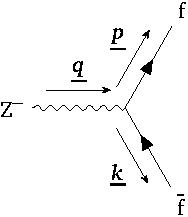
\includegraphics{z0-decay}
    \caption{%
        Decay of a $\mathrm Z^0$ gauge boson into a pair of fermions. Time is
        to the right.
    }
    \label{fig:z0-decay}
\end{figure}

First we compute the invariant matrix element~$\mathcal M$. Reading off the
Feynman diagram, we have
\begin{align*}
    \iup \mathcal M
    &= \epsilon^\mu \bar u^s(\four p) \frac{\iup g}{\cos(\theta_\text w)}
    \mat\gamma_\mu \del{g_\text v^f - g_\text a^f \mat\gamma_5} v^{s'}(\four k)
    \,,
    \intertext{%
        where we have used the rules given by \textcite[(D.56)]{romao/aqt}. We
        chose the center of mass system, as we always can for a single massive
        particle, and have $\four q = (\sqrt s, \vec 0)$. As the gauge boson
        does not have any three momentum direction, we can choose the
        polarization vector $\four \epsilon$ like we want. We chose it in the
        positive $x^3$-direction and have $\four \epsilon = (0, 0, 0, 1)$. With
        that we can simplify the Lorentz structure a little bit and obtain
    }
    &= \bar u^s(\four p) \frac{\iup g}{\cos(\theta_\text w)}
    \mat\gamma_3 \del{g_\text v^f - g_\text a^f \mat\gamma_5} v^{s'}(\four k)
    \,.
\end{align*}

For the decay width, which we are interested in, we need the modulus squared of
the matrix element. For that we need the following:
\begin{multline*}
    \sbr{\bar u^s(\four p) \mat\gamma_3 \del{g_\text v^f - g_\text a^f \mat\gamma_5}
    v^{s'}(\four k)}^\dagger \\
    =
    v^{s'}(\four k)^\dagger
    \del{g_\text v^f - g_\text a^f \mat\gamma_5^\dagger}
    \mat\gamma_3^\dagger
    \mat\gamma_0
    u^s(\four p) \\
    =
    \underbracket{v^{s'}(\four k)^\dagger
    \mat\gamma_0}
    \underbracket{\mat\gamma_0
        \del{g_\text v^f - g_\text a^f \mat\gamma_5^\dagger}
    \mat\gamma_0}
    \underbracket{\mat\gamma_0
        \mat\gamma_3^\dagger
    \mat\gamma_0}
    u^s(\four p) \\
    = \bar v^{s'}(\four k)
    \del{g_\text v^f + g_\text a^f \mat\gamma_5}
    \mat\gamma_3
    u^s(\four p) \\
    = \bar v^{s'}(\four k)
    \mat\gamma_3
    \del{g_\text v^f - g_\text a^f \mat\gamma_5}
    u^s(\four p) \,. \\
\end{multline*}

Now we can write the modulus squared of the matrix element
\begin{align*}
    |\mathcal M|^2
    &= \frac{g^2}{\cos(\theta_\text w)^2}
    \bar v^{s'}(\four k)
    \mat\gamma_3
    \del{g_\text v^f - g_\text a^f \mat\gamma_5}
    u^s(\four p)
    \bar u^s(\four p)
    \mat\gamma_3
    \del{g_\text v^f - g_\text a^f \mat\gamma_5}
    v^{s'}(\four k)
    \,. \\
    \intertext{%
        As the detector is not sensitive to the spin of the resulting fermions,
        we need to sum over all the final state spin configurations $s$ and
        $s'$. This will give us a fermion trace,
    }
    \sum_\text{spins} |\mathcal M|^2
    &=
    \frac{g^2}{\cos(\theta_\text w)^2}
    \tr\del{
        \four k
        \mat\gamma_3
        \del{g_\text v^f - g_\text a^f \mat\gamma_5}
        \four p
        \mat\gamma_3
        \del{g_\text v^f - g_\text a^f \mat\gamma_5}
    }
    \,, \\
    \intertext{%
        where we have neglected the masses of the fermions. The second
        parentheses with $\mat\gamma_5$ can be anticommuted twice and be
        collapsed with the first one. We have
    }
    &=
    \frac{g^2}{\cos(\theta_\text w)^2}
    \tr\del{
        \four k
        \mat\gamma_3
        \del{g_\text v^f - g_\text a^f \mat\gamma_5}^2
        \four p
        \mat\gamma_3
    }
    \,, \\
    \intertext{%
        where we can now simplify this. As an aside, we have
        \[
            \del{g_\text v^f - g_\text a^f \mat\gamma_5}^2
            = (g_\text v^f)^2 - (g_\text a^f)^2 - 2 g_\text v^f g_\text a^f
            \mat\gamma_5 \,.
        \]
        The square of $\mat\gamma_5$ is just the unit matrix in Dirac space.
        The term with $\mat\gamma_5$ will drop out as the trace identity
        contains the Levi-Civita symbol~$\epsilon_{\mu\nu\rho\gamma}$ which
        will be zero if two of the indices are 3, as we have in our case.
        Therefore we can directly drop that term. As it does not contain any
        further Dirac structure, we can pull it out front and obtain
    }
    &=
    \frac{g^2}{\cos(\theta_\text w)^2}
    \del{(g_\text v^f)^2 - (g_\text a^f)^2}
    \tr\del{
        \four k
        \mat\gamma_3
        \four p
        \mat\gamma_3
    }
    \,.
    \intertext{%
        Using a trace identity like given by \textcite[(A.27)]{Peskin/QFT/1995}
        we obtain
    }
    &= \frac{4 g^2}{\cos(\theta_\text w)^2} \del{(g_\text v^f)^2 - (g_\text a^f)^2}
    (2 k_3 p_3 + \four k \cdot \four p) \,.
\end{align*}
This is our final form of the matrix element.

The decay width is given by additional factors and a integration over phase
space. We have
\begin{align*}
    \Gamma_f
    &= \frac{1}{2 M_{\mathrm Z^0}} (2 \piup)^4 \int
    \frac{\dif^3 p}{(2\piup)^3 2 E_{\vec p}}
    \frac{\dif^3 k}{(2\piup)^3 2 E_{\vec k}}
    \delta^4(\four q - \four k - \four p)
    |\mathcal M|^2 \,.
    \intertext{%
        We simplify the factors and insert the matrix element and get
    }
    &= \frac{1}{32 \piup^2 M_{\mathrm Z^0}} \int
    \frac{\dif^3 p}{E_{\vec p}}
    \frac{\dif^3 k}{E_{\vec k}}
    \delta^4(\four q - \four k - \four p)
    \frac{4 g^2}{\cos(\theta_\text w)^2}
    \del{(g_\text v^f)^2 - (g_\text a^f)^2}
    (2 k_3 p_3 + \four k \cdot \four p) \,.
    \intertext{%
        Then we simplify even more and obtain
    }
    &= \frac{1}{8 \piup^2 M_{\mathrm Z^0}}
    \frac{g^2}{\cos(\theta_\text w)^2}
    \del{(g_\text v^f)^2 - (g_\text a^f)^2}
    \int
    \frac{\dif^3 p}{E_{\vec p}}
    \frac{\dif^3 k}{E_{\vec k}}
    \delta^4(\four q - \four k - \four p)
    (2 k_3 p_3 + \four k \cdot \four p) \,.
    \intertext{%
        The total energy-momentum conserving Dirac-distribution can be split
        into time-like and space-like part. In the center-of-mass frame, this
        gives us
    }
    &= \frac{1}{8 \piup^2 M_{\mathrm Z^0}}
    \frac{g^2}{\cos(\theta_\text w)^2}
    \del{(g_\text v^f)^2 - (g_\text a^f)^2}
    \\&\qquad\times
    \int
    \frac{\dif^3 p}{E_{\vec p}}
    \frac{\dif^3 k}{E_{\vec k}}
    \delta(\sqrt s - E_{\four k} - E_{\four p})
    \delta^3(\vec k + \vec p)
    (2 k_3 p_3 + \four k \cdot \four p) \,,
    \intertext{%
        which suggests the following change in variables:
        \[
            \vec a := \vec p + \vec k
            \eqnsep
            \vec b := \frac{\vec p - \vec k}{2} \,.
        \]
        The Jacobian of this transformation is unity. The $\delta^3(\vec k +
        \vec p)$ will become $\delta^3(\vec a)$, in the $\int \dif^3 a$
        integral, this will set $\vec a$ to $\vec 0$. So far we have
    }
    &= \frac{1}{8 \piup^2 M_{\mathrm Z^0}}
    \frac{g^2}{\cos(\theta_\text w)^2}
    \del{(g_\text v^f)^2 - (g_\text a^f)^2}
    \int
    \frac{\dif^3 b}{E_{\vec p} E_{\vec k}}
    \delta(\sqrt s - E_{\vec k} - E_{\vec p})
    (2 k_3 p_3 + \four k \cdot \four p) \,.
    \intertext{%
        Now we have to replace $k$ and $p$ with $b$. We have $\vec p = \vec b$
        and $\vec k = - \vec b$. Their magnitude is the same, which is expected
        in the center-of-mass frame in a two body decay. This simplifies the
        relations to
    }
    &= \frac{1}{8 \piup^2 M_{\mathrm Z^0}}
    \frac{g^2}{\cos(\theta_\text w)^2}
    \del{(g_\text v^f)^2 - (g_\text a^f)^2}
    \int
    \frac{\dif^3 b}{E_{\vec b}^2}
    \delta(\sqrt s - 2 E_{\vec b})
    (- 2 b_3 b_3 + E_{\vec b}^2 + \vec b \cdot \vec b) \,.
    \intertext{%
        As we have massless particles, we have $E_{\vec b} = |\vec b|$. We
        change into spherical coordinates in $\vec b$ and obtain
    }
    &= \frac{1}{4 \piup M_{\mathrm Z^0}}
    \frac{g^2}{\cos(\theta_\text w)^2}
    \del{(g_\text v^f)^2 - (g_\text a^f)^2}
    \\&\qquad\times
    \int \dif b \, b^2 \int \dif \cos(\theta) \,
    \frac{1}{b^2}
    \delta(\sqrt s - 2 b)
    (- 2 b^2 \cos(\theta)^2 + b^2 + b^2) \,,
    \intertext{%
        where we have performed $\int \dif \phi = 2 \piup$ already as we do not
        have any explicit $\phi$-dependence. The radial integration will set $b
        = \sqrt s / 2$. In our case $s = M_{\mathrm Z^0}^2$ and we have
    }
    &= \frac{M_{\mathrm Z^0}}{16 \piup}
    \frac{g^2}{\cos(\theta_\text w)^2}
    \del{(g_\text v^f)^2 - (g_\text a^f)^2}
    \int \dif \cos(\theta) \,
    (- 2 \cos(\theta)^2 + 2) \,.
    \intertext{%
        The angular integration gives $(-4/3 + 4) = 8/3$, so we get
    }
    &= \frac{M_{\mathrm Z^0}}{6 \piup}
    \frac{g^2}{\cos(\theta_\text w)^2}
    \del{(g_\text v^f)^2 - (g_\text a^f)^2} \,.
    \intertext{%
        Replacing $g^2$ with $8 M_{\mathrm W}^2 G_\text F / \sqrt 2$ (see
        Equation~(2.1) from the manual) and using $M_\mathrm W = \MZ
        \cos(\theta_\mathrm w)$ (see (2.3)), we will obtain
    }
    &= \frac{2 \sqrt 2}{3 \piup}
    G_\text F M_{\mathrm Z^0}^3
    \del{(g_\text v^f)^2 - (g_\text a^f)^2} \,.
    \intertext{%
        For quarks, we also need to sum over all the colors, which just gives
        the factor $N_\mathrm c^f$ for the given flavor $f$.
    }
    &= \frac{N_\mathrm c^f 2 \sqrt 2}{3 \piup}
    G_\text F M_{\mathrm Z^0}^3
    \del{(g_\text v^f)^2 - (g_\text a^f)^2} \,.
\end{align*}

Except for a missing factor $1/8$ up front, this is the same as
Equation~(2.12) given in the manual.

% FIXME Find the missing factors.

We can now insert the various quantum numbers of particles, insert the numbers
and obtain the decay widths. Our results are listed in
Table~\ref{tab:decay_widths}.

The Fermi coupling constant has the value \SI{<< fermi_coupling
>>}{\per\giga\electronvolt\squared}, see Equation~(2.1) in the manual.

\begin{table}
    \centering
    \begin{tabular}{lcccS}
        \toprule
        Flavor & $I_3$ & $Q$ & $N_\text c$ & $\Gamma / \si{\mega\electronvolt}$ \\
        \midrule
        Electron & $-1/2$ & $-1$ & 1 & << gamma_electron >> \\
        Neutrino & $1/2$ & $0$ & 1 & << gamma_neutrino >> \\
        Up-Quark & $1/2$ & $2/3$ & 3 & << gamma_up_type >> \\
        Down-Quark & $-1/2$ & $-1/3$ & 3 & << gamma_down_type >> \\
        \bottomrule
    \end{tabular}
    \caption{%
        Decay widths for the various families of fermions. As the fermions are
        taken to be massless, only one representative of the family is
        mentioned in the column \enquote{Flavor}.
    }
    \label{tab:decay_widths}
\end{table}

\section{Partial widths}
\label{sec:exercise-partial-widths}

In the previous section, we have computed the decay widths for each kind of
particle. Now we have to group the various particles into families and add
their partial widths.

\begin{description}
    \item[Hadronic width]
        The hadrons in the final state are the up, down, strange, charm and
        bottom quarks. Therefore we have two up-type and three down-type quarks
        which results in a width of
        $\Gamma_\text{had.} = \SI{<< hadronic_width >>}{\mega\electronvolt}$.
        The branching ratio here is \num{<< hadronic_ratio >>}.

    \item[Charged leptonic width]
        The charged leptons are the electron, the muon and the tauon. The charged
        leptonic width therefore is
        $\Gamma_\text{ch.lep.} = \SI{<< charged_leptonic_width >>}{\mega\electronvolt}$.
        The branching ratio here is \num{<< charged_leptonic_ratio >>}.

    \item[Neutral leptonic width]
        The neutral leptons are the electron-neutrino, the muon-neutrino and
        the tauon-neutrino. The neutral
        leptonic width therefore is
        $\Gamma_\text{n.lep.} = \SI{<< neutral_leptonic_width >>}{\mega\electronvolt}$.
        The branching ratio here is \num{<< neutral_leptonic_ratio >>}.

    \item[Total width]
        Summing all those widths up, we obtain
        $\Gamma_\text{tot.} = \SI{<< total_width >>}{\mega\electronvolt}$.
\end{description}

All numerical values as well as the partial cross sections are in
Table~\ref{tab:partial_stuff}. The total cross section is
\[
    \sigma_\text{total}^\text{peak} = \frac{12 \piup}{\MZ^2} \frac{\Gamma_\text
    e}{\Gamma_{\mathrm Z^0}} \,.
\]

\begin{table}
    \centering
    \begin{tabular}{lSSS}
        \toprule
        Type & {Width / \si{\mega\electronvolt}} & {Branching ratio} & {Partial
    cross section / \SI{e-11}{\per\mega\electronvolt\squared}} \\
        \midrule
        Hadronic
        & << hadronic_width >> & << hadronic_ratio >> & <<
        hadronic_partial_cross_section >> \\
        Charged leptonic
        & << charged_leptonic_width >> & << charged_leptonic_ratio >> & <<
        charged_leptonic_partial_cross_section >> \\
        Neutral leptonic
        & << neutral_leptonic_width >> & << neutral_leptonic_ratio >> & <<
        neutral_leptonic_partial_cross_section >> \\
        Total
        & << total_width >> & 1 & <<
        total_cross_section >> \\
        \bottomrule
    \end{tabular}
    \caption{%
        Partial decay widths, branching ratios and cross sections.
    }
    \label{tab:partial_stuff}
\end{table}

\section{Additional generation}

If we have an additional generation, we have one more up-type and down-type
quark. Also one more lepton-type and another neutrino-type. Therefore we need
to add to the total width. The ratio is
\[
    \frac{\Gamma_\text{total} + \Gamma_\mathrm e + \Gamma_\nuup +
    \Gamma_\mathrm u + \Gamma_\mathrm d}{\Gamma_\text{total}}
    = 1 + \frac{\Gamma_\mathrm e + \Gamma_\nuup + \Gamma_\mathrm u +
    \Gamma_\mathrm d}{\Gamma_\text{total}}
    = \num{<< extra_width >>} \,.
\]
We see that another generation of quarks and leptons significantly changes the
total width and therefore also the total cross section.

\section{Angular dependence}

As we can see from the tree-level \textsc{qft} calculation for the $\mathrm
Z^0$ decay in the first problem, the angular dependence is indeed $(1 +
\cos(\theta)^2)$ as stated in the last paragraph on page~27 in the manual.
This is the $s$-channel. For the $t$-channel the angular dependence is $(1 -
\cos(\theta))\inv$.

The reaction $\mathrm{e^+ e^- \to \muup^+ \muup^-}$ only works in the
$s$-channel. The reaction $\mathrm{e^+ e^- \to e^+ e^-}$ works in both $s$- and
$t$-channel.

All we have to do is to plot those two simple functions. The plots are shown in
Figure~\ref{fig:channels}. As written in the manual, the $t$-channel becomes
dominant for very small angles, i.e.\ large $\cos(\theta)$.

\begin{figure}
    \centering
    \includegraphics{s-channel}
    \caption{%
        Angular dependence of differential cross section in the $s$- and
        $t$-channel.
    }
    \label{fig:channels}
\end{figure}

\section{Asymmetry}
\label{sec:exercises-asymmetry}

We are to compute the forward--backward asymmetry of the reaction $\mathrm e^+
\mathrm e^- \to \muup^+ \muup^-$. The given values for Mandelstam-$s$ are
\SIlist{<< ';'.join(s_array) >>}{\giga\electronvolt}. The values for the weak
mixing angle in terms of $\sin(\theta_\text w)^2$ given are \numlist{<<
';'.join(sin_sq_array) >>}. In total there are nine combinations, all are shown
in Table~\ref{tab:asymmetry}.

\begin{table}
    \centering
    \begin{tabular}{S*3S}
        \toprule
        & \multicolumn{3}{c}{$A_\text{FB}^\muup$} \\
        \cmidrule(l){2-4}
        {$s$}
        %< for x in sin_sq_array >%
        & {$\sin(\theta_\text w)^2 = \num{<< x >>}$}
        %< endfor >%
        \\
        \midrule
        %< for row in asymmetry_table >%
        << ' & '.join(row) >> \\
        %< endfor >%
        \bottomrule
    \end{tabular}
    \caption{%
        Forward--backward asymmetry $A_\text{FB}^\muup$ for different
        values of Mandelstam-$s$ (rows) and different values of $\theta_\text
        w$ (columns).
    }
    \label{tab:asymmetry}
\end{table}

The equation that we use is (2.19) from the manual:
\[
    A_\text{FB}^f(s) \simeq - \frac 32 \frac{a_\mathrm e a_f Q_f \Re(\chi(s))}{(v_\mathrm e^2
    + a_\mathrm e^2)(v_f^2 + a_f^2)} \,,
\]
where $\chi(s)$ is the propagator of the $\mathrm Z^0$ boson as given in
(2.11). It differs from the usual propagator of a vector particle and does not
have any Lorentz structure. This is odd, we will just use the given propagator.
The real part of that propagator has to be found by making the denominator
real:
\[
    \chi(s)
    = \frac{s}{s - \MZ^2 + \frac{\iup s \Gamma_{\mathrm Z^0}}\MZ}
    = s \frac{s - \MZ^2 - \frac{\iup s \Gamma_{\mathrm Z^0}}\MZ}
    {\del{s - \MZ^2}^2 + \del{\frac{s \Gamma_{\mathrm Z^0}}\MZ}^2} \,.
\]
The real part then is
\[
    \Re(\chi(s))
    = \frac{s(s - \MZ^2)}
    {\del{s - \MZ^2}^2 + \del{\frac{s \Gamma_{\mathrm Z^0}}\MZ}^2} \,.
\]

Now we just need to insert all the numbers with $I_3 = -1/2$ and $Q = -1$ in
both $f = \mathrm e$ and $f = \muup$.

%%%%%%%%%%%%%%%%%%%%%%%%%%%%%%%%%%%%%%%%%%%%%%%%%%%%%%%%%%%%%%%%%%%%%%%%%%%%%%%

\chapter{Analysis}

The data used in this lab experiment was gathered in the year 1992 and before.
Therefore we only do analysis of the data. Part of the analysis is done at the
university, the remainder is done at home. We will group our work by topic and
not split by university and home.

\section{Screening some decays}

At first we looked at some decays in the event display software
\textsc{grope}. In order to learn the signatures of the various decays, we
start with Monte Carlo datasets which only contain decays into a given channel.

The characteristics have different names within \textsc{grope} and
\textsc{paw}. Both are programming language identifiers and hard to
read. Since we do not want to clutter our report with those identifiers, we use
ones close to \textsc{paw} but formatted nicer. See
Table~\ref{tab:nomenclature} for an overview.

\begin{table}
    \centering
    \begin{tabular}{llll}
        \toprule
        \textsc{grope}
        & \textsc{paw}
        & Our name
        & Description
        \\
        \midrule
        \texttt{Ctrk(N)} & \texttt{ncharged} & \ncharged\ & Number of charged
        tracks\\
        \texttt{Ctrk(Sump)} & \texttt{pcharged} & \pcharged\ & Energy in
        charged tracks \\
        \texttt{Ecal(SumE)} & \texttt{e\_ecal} & \eecal\ & Energy in electric
        calorimeter \\
        \texttt{Hcal(SumE)} & \texttt{e\_hcal} & \ehcal\ & Energy in hadronic
        calorimeter \\
        \bottomrule
    \end{tabular}
    \caption{%
        Nomenclature used by \textsc{grope}, \textsc{paw} and within this lab
        report.
    }
    \label{tab:nomenclature}
\end{table}

Figure~\ref{fig:grope} shows the events as displayed by \textsc{grope}. We have
picked a representative event for each category of decay (electrons, muons,
tauons, hadrons).

\begin{figure}
    \centering
    \begin{subfigure}[c]{0.48\linewidth}
        \centering
        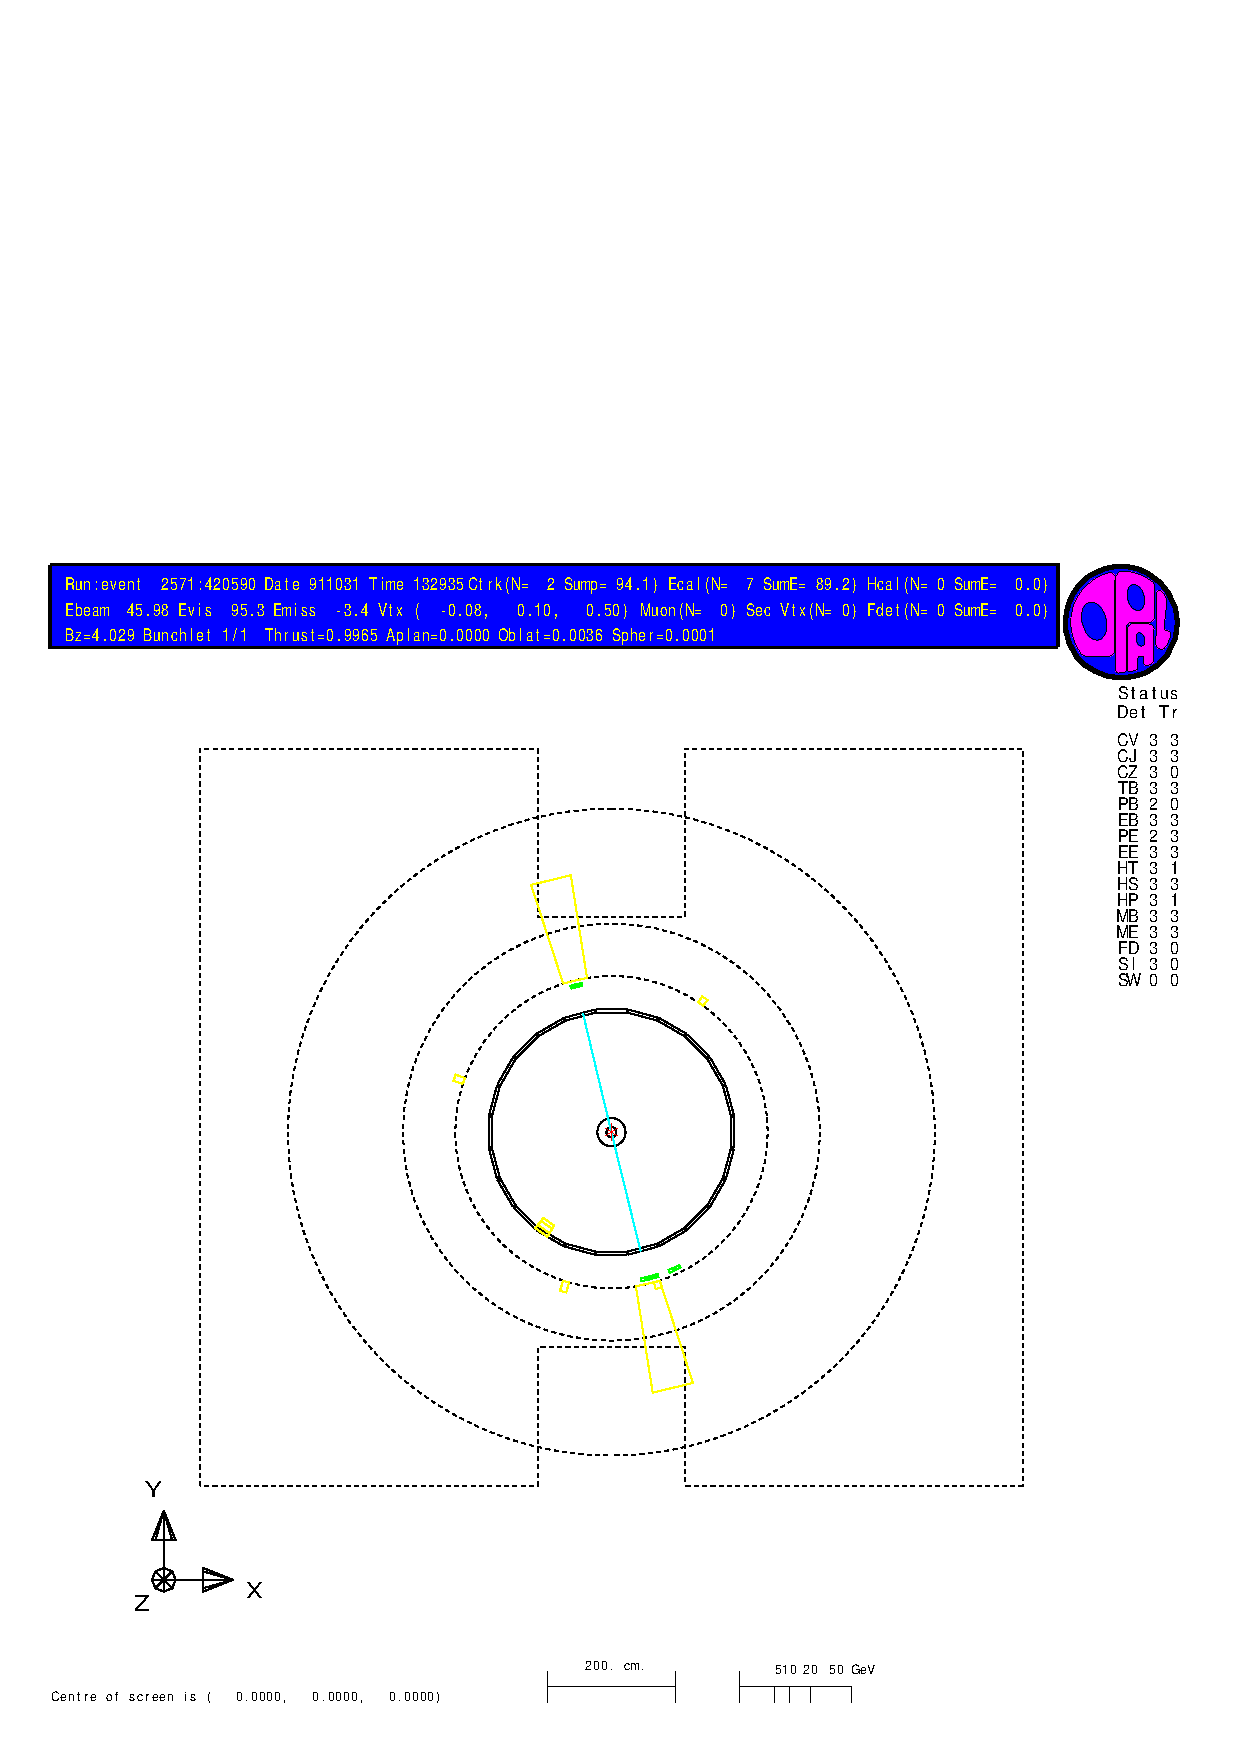
\includegraphics[width=\linewidth]{opal-electrons}
        \caption{%
            Electrons
        }
        \label{fig:grope/electrons}
    \end{subfigure}
    \hfill
    \begin{subfigure}[c]{0.48\linewidth}
        \centering
        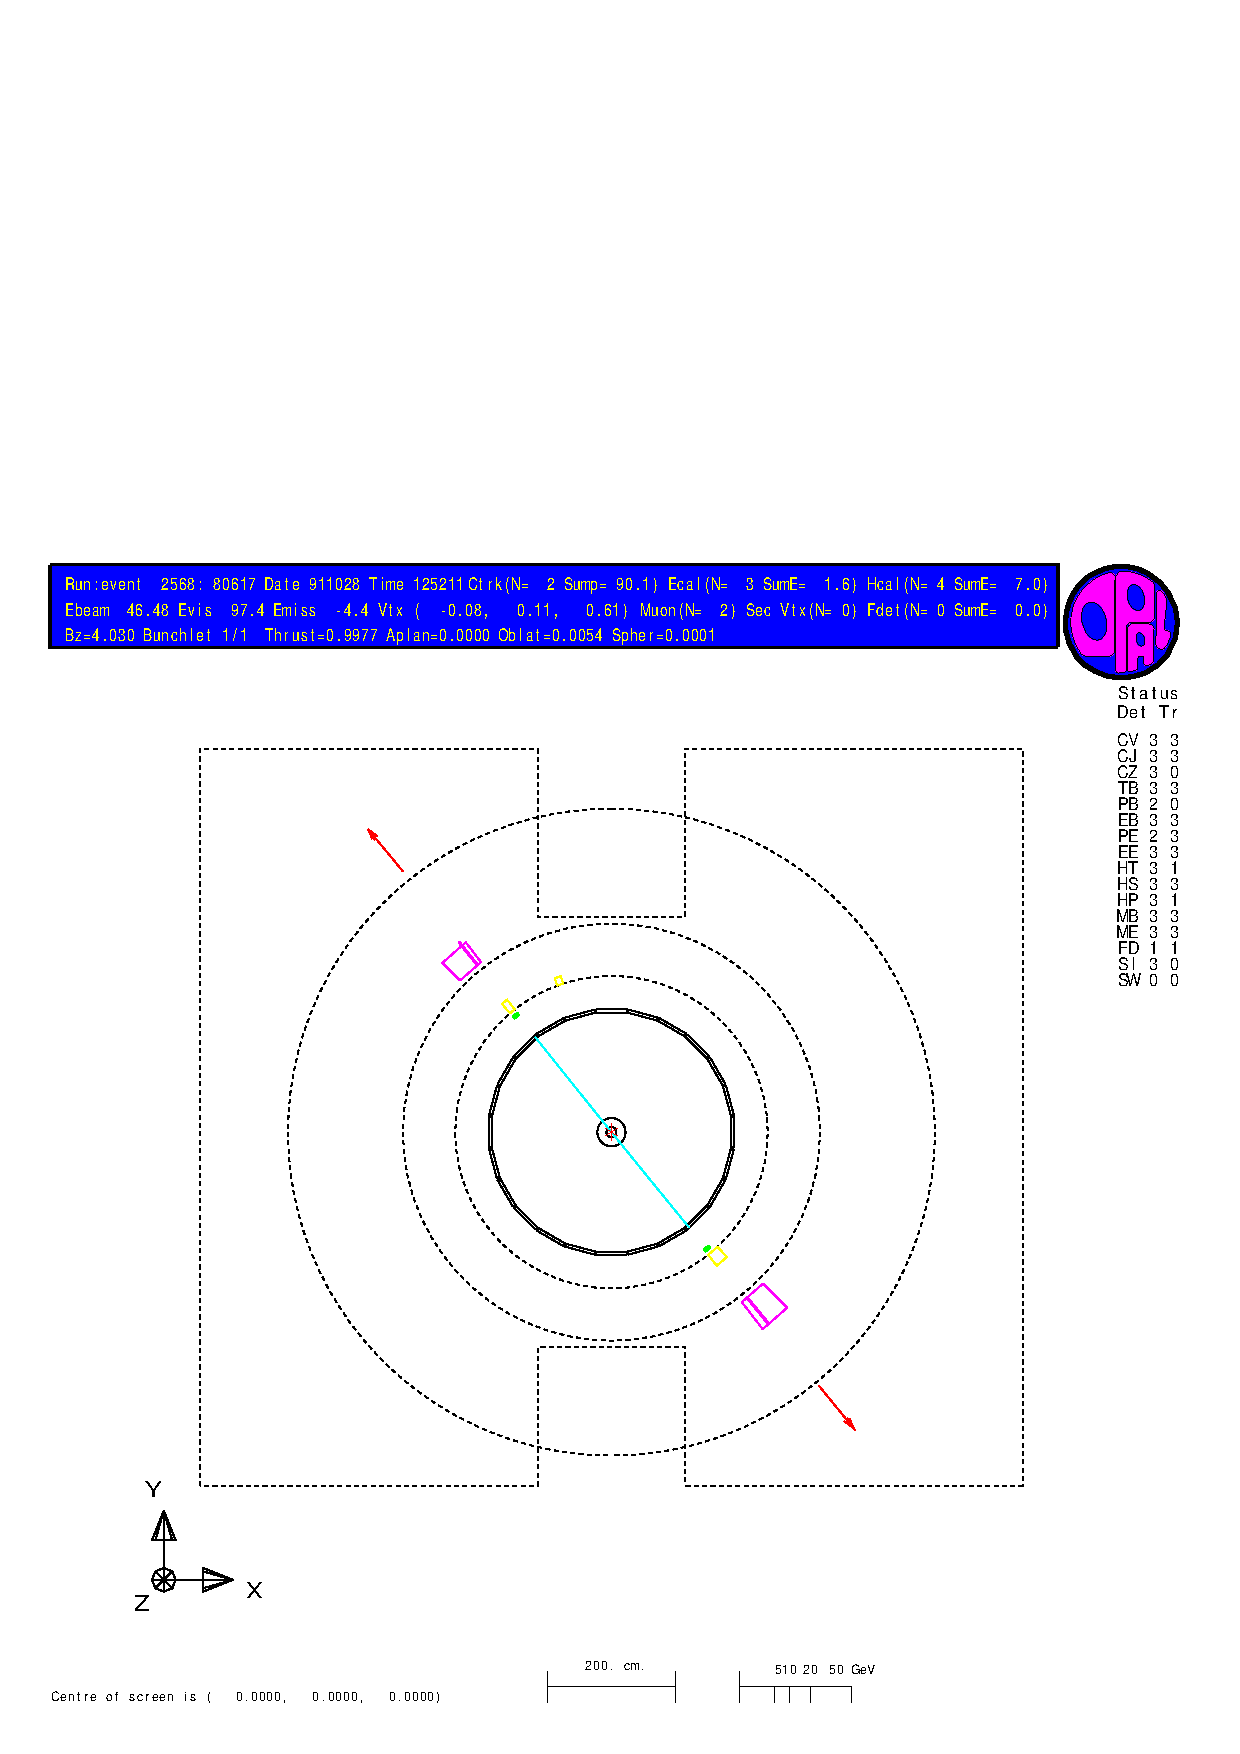
\includegraphics[width=\linewidth]{opal-muons}
        \caption{%
            Muons
        }
        \label{fig:grope/muons}
    \end{subfigure}

    \vspace{2ex}

    \begin{subfigure}[c]{0.48\linewidth}
        \centering
        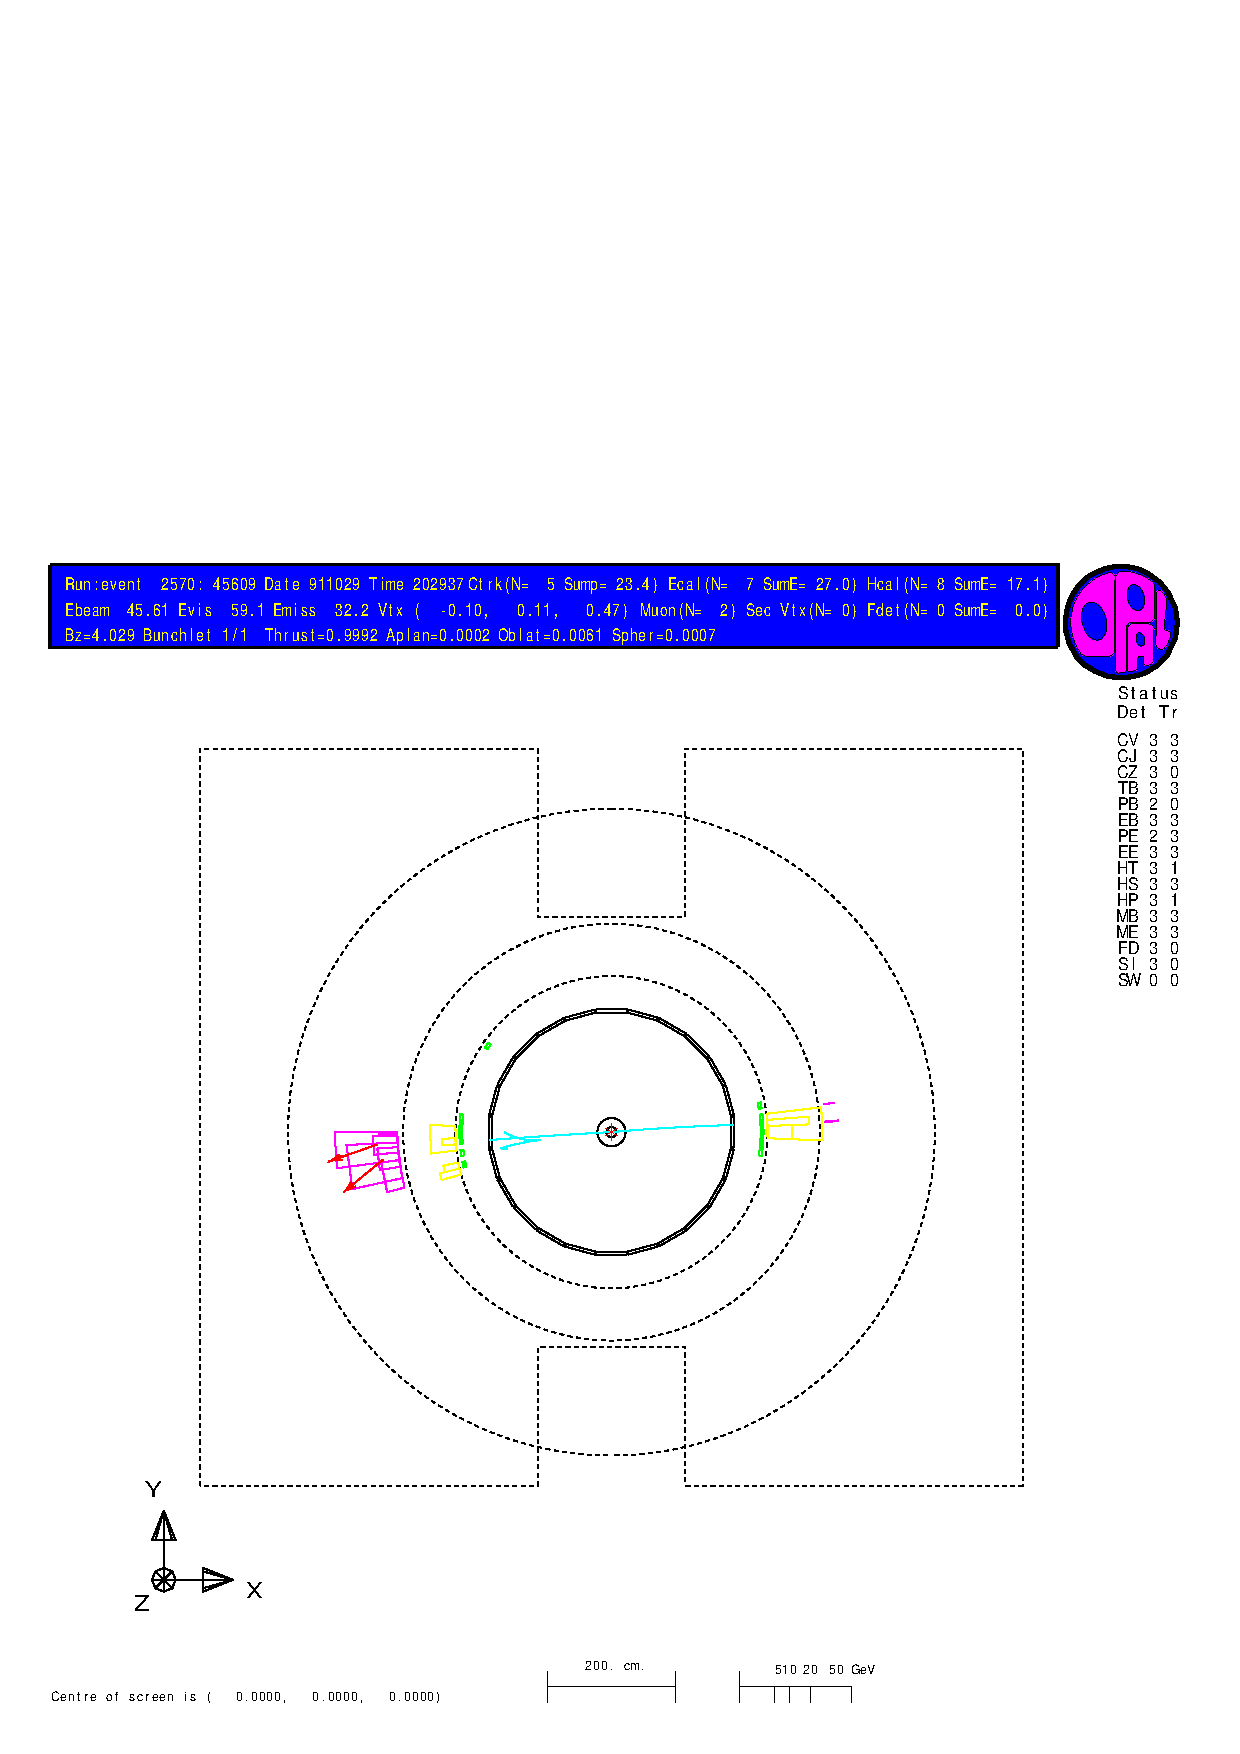
\includegraphics[width=\linewidth]{opal-taus}
        \caption{%
            Tauons
        }
        \label{fig:grope/tauons}
    \end{subfigure}
    \hfill
    \begin{subfigure}[c]{0.48\linewidth}
        \centering
        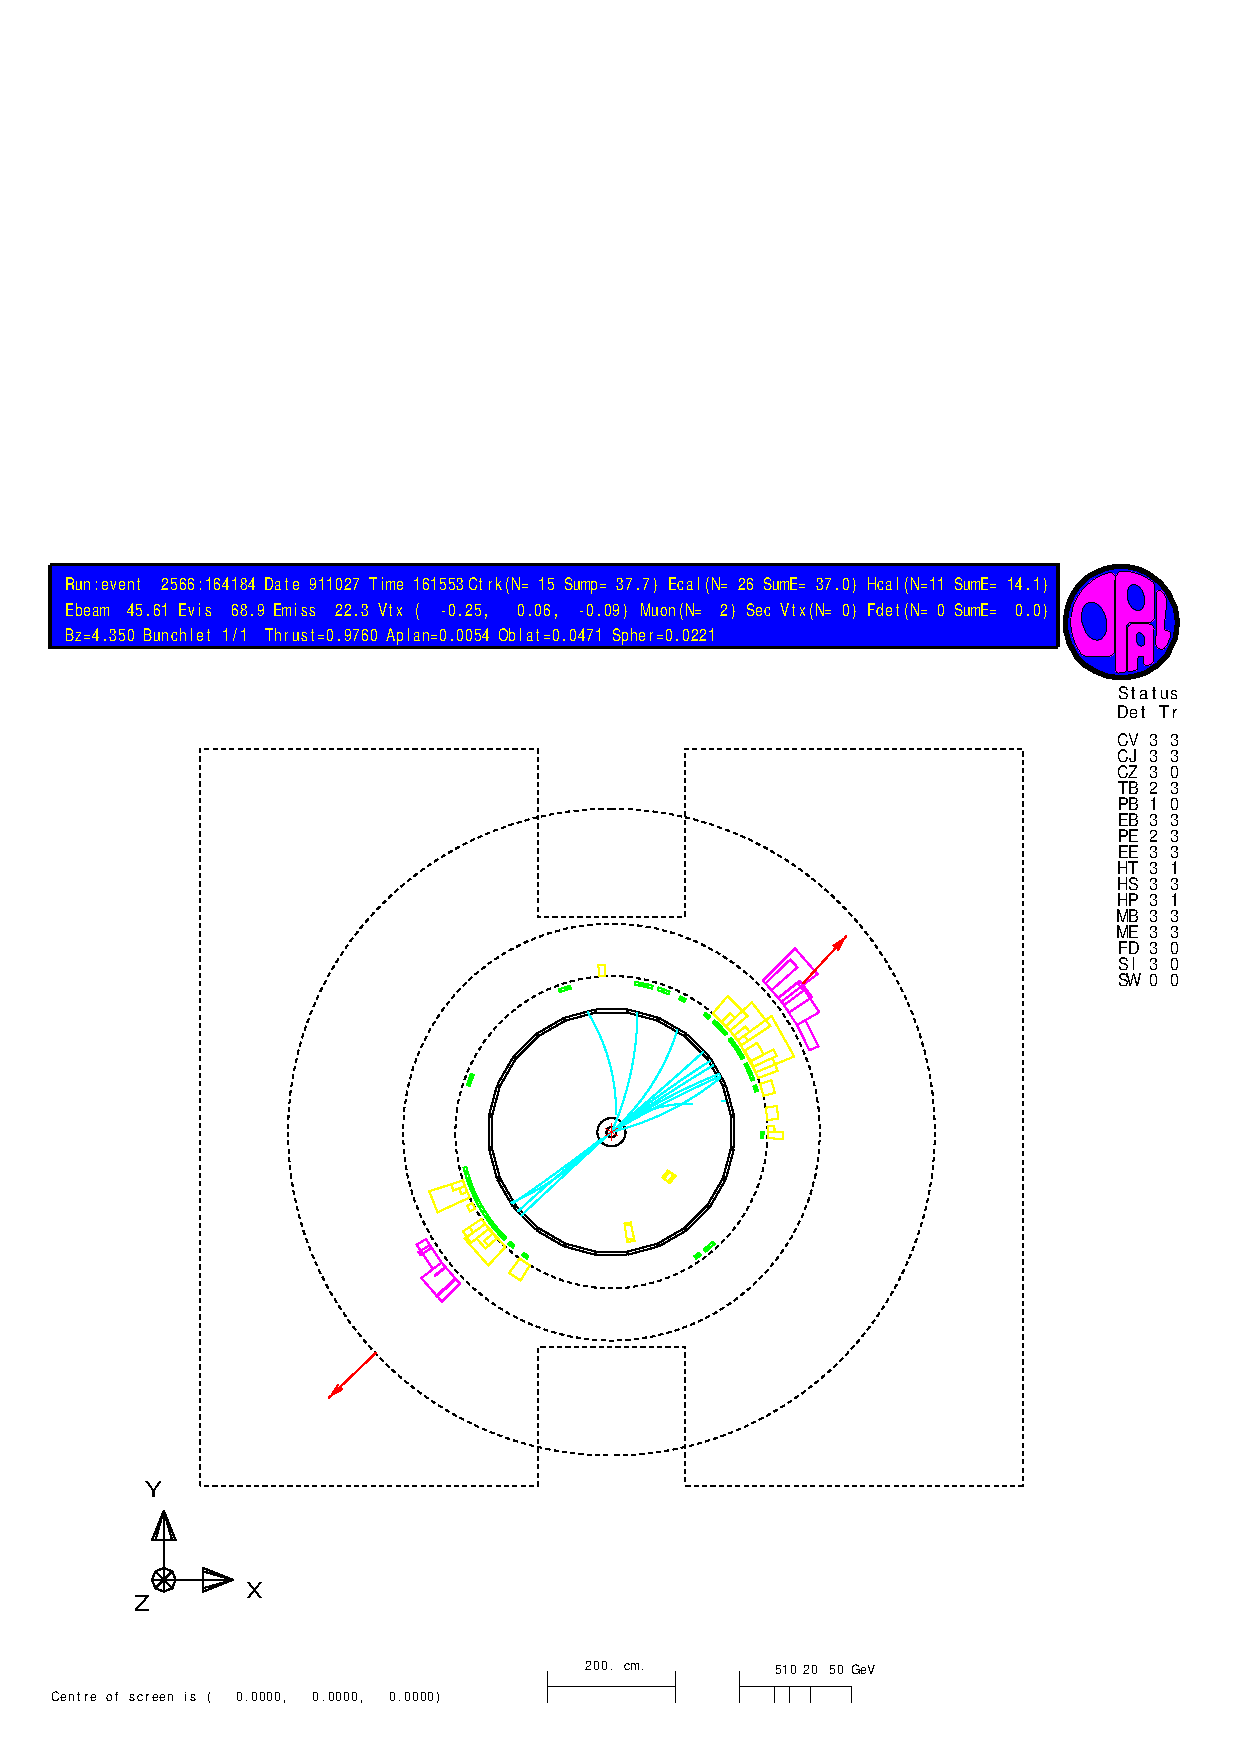
\includegraphics[width=\linewidth]{opal-hadrons}
        \caption{%
            Hadrons
        }
        \label{fig:grope/hadrons}
    \end{subfigure}
    \caption{%
        Event display of Monte Carlo events. One can see the traces from the
        vertex chamber in cyan, the hits in the \ecal{} are shown in yellow
        (probably hard to see on paper). In magenta, one has the hits in the
        \hcal{}. Muon penetrations are indicated with red arrows. Images are
        rendered with \textsc{grope}.
    }
    \label{fig:grope}
\end{figure}


The electron decay in Figure~\ref{fig:grope/electrons} shows the typical
back-to-back signature of two very fast (no curvature in the vertex chamber)
charged particles. All the energy is deposited in the \ecal{}. In the dark blue
header one can see that the missing energy is very small. The \eecal{} is
pretty much identical with \pcharged{}. Both energies are almost the beam energy.

Decays into muons have a different signature. The most prominent feature are
the hits in the muon chambers, as one can see in Figure~\ref{fig:grope/muons}.
The \pcharged{} is the beam energy, little energy is unaccounted for. This means
that there are no neutrinos created in that decay. \eecal{} and \ehcal{} is
small, this is due to the big mass of the muon (compared to electrons).

Figure~\ref{fig:grope/tauons} shows a decay into tauons. This decay is not as
simple as the previous ones. We have some missing energy (around a third), more
than one charged track and also energy deposited into the various calorimeters.
The missing energy comes from the neutrinos in the weak decay of the tauon. The
number of charged tracks is still small (just five), therefore we can
differentiate from the hadronic decays.

Lastly, a decay into hadrons is shown in Figure~\ref{fig:grope/hadrons}. One
directly sees the large number of tracks, here 26, which exhibit a larger
curvature. Also we have nonzero \ehcal{}. Hadronic decays are easy to classify
as their number of charged tracks is always rather large.

\section{Defining the cuts}

While reviewing the Monte Carlo events in \textsc{grope}, we generate
histograms with the various characteristics. We choose to write down
\ncharged{}, \pcharged{}, \eecal{} and \ehcal{}. Those characteristics are also
available in the later analysis of larger datasets using \textsc{paw}.

\subsection{Preliminary analysis}

We will use the following color scheme throughout this report:
Electrons~\includegraphics{legend-electron},
Muons~\includegraphics{legend-muon},
Tauons~\includegraphics{legend-tauon} and
Hadrons~\includegraphics{legend-hadron}.

Using some twenty points per event class, we obtain the histograms shown in
Figure~\ref{fig:hist}. There one can see that some characteristics are well
suited to cut the data. For instance in \ncharged, we see that hadronic decays
have more than seven tracks, whereas the leptonic decays have less. In the
histogram for \pcharged, we see that a cut at around \SI{80}{\giga\electronvolt}
can separate tauons and muons. Another cut in \eecal{} at around
\SI{75}{\giga\electronvolt} allows us to separate tauons and electrons. The
energy deposited into the \hcal\, \eecal, is not very helpful for cutting.

\begin{figure}
    \centering
    \begin{subfigure}[c]{0.49\linewidth}
        \centering
        \includegraphics{hist-ctrk_n}
        \caption{%
            \ncharged
        }
        \label{fig:hist/ncharged}
    \end{subfigure}
    \hfill
    \begin{subfigure}[c]{0.49\linewidth}
        \centering
        \includegraphics{hist-ctrk_sump}
        \caption{%
            \pcharged/\si{\giga\electronvolt}
        }
        \label{fig:hist/pcharged}
    \end{subfigure}

    \vspace{2ex}

    \begin{subfigure}[c]{0.49\linewidth}
        \centering
        \includegraphics{hist-ecal_sume}
        \caption{%
            \eecal/\si{\giga\electronvolt}
        }
        \label{fig:hist/eecal}
    \end{subfigure}
    \hfill
    \begin{subfigure}[c]{0.49\linewidth}
        \centering
        \includegraphics{hist-hcal_sume}
        \caption{%
            \ehcal/\si{\giga\electronvolt}
        }
        \label{fig:hist/ehcal}
    \end{subfigure}
    \caption{%
        Histograms with data gathered from Monte Carlo datasets in
        \textsc{grope}. The number of charged tracks is shown as a histogram
        with logarithmic bins.
    }
    \label{fig:hist}
\end{figure}


Having those cuts in place, we take a look at the \texttt{test} datasets which
are not sorted by event type. There we try to use our fresh intuition about the
decay channels to identify the type of decay. Then we take a look at the
characteristics and see whether our cuts would come to the same conclusion. For
most decays, this worked out well. Some were not classified correctly; this is
somewhat expected as we will never be able to avoid false-positives and
false-negatives.

While we were trying to find suitable cuts, a 3D visualization like shown in
Figure~\ref{fig:mpl-scatter} was really helpful. There we could turn the cloud
of events in the characteristics space and see different clusters. Such a
3D-representation can hardly be printed and must be viewed interactively,
though.

\begin{figure}
    \centering
    \includegraphics[width=.6\linewidth]{mpl-scatter}
    \caption{%
        3D visualization of the three most expressive characteristics.
    }
    \label{fig:mpl-scatter}
\end{figure}

We would really have liked to perform this visualization with more data. Then
one could even do a 3D-histogram and find cut surfaces which separate the data
most cleanly. In \textsc{paw} we were limited to hyperplanes anyway, so we just
chose a few axis-parallel planes as they did the job sufficiently well.

After the refining using events from the \texttt{test} dataset, we have the
cuts listed in Table~\ref{tab:cuts}.

\begin{table}
    \centering
    \begin{tabular}{lcccc}
        \toprule
        & \multicolumn{4}{c}{Cut criterion} \\
        \cmidrule(l){2-5}
        Particle
        & \ncharged
        & \pcharged/\si{\giga\electronvolt}
        & \eecal/\si{\giga\electronvolt}
        & \ehcal/\si{\giga\electronvolt} \\
        \midrule
        Electrons & $< 4$ &  & $> 60$ &  \\
        Muons & $< 4$ & $> 75$ & $< 20$ &  \\
        Tauons & $< 7$ & $< 75$ & $\leq 75$ &  \\
        Hadrons & $> 7$ &  &  &  \\
        \bottomrule
    \end{tabular}
    \caption{%
        Cuts derived from the few data points manually extracted from the Monte
        Carlo events.
    }
    \label{tab:cuts}
\end{table}

\subsection{More data points}

Our histograms are only filled with a limited amount of data. It would be wise
to use more data to refine the cuts further. To that end, we change from
the single event viewer \textsc{grope} to the analysis tool \textsc{paw} which
is a predecessor to \textsc{root}.

We load the big Monte Carlo datasets into \textsc{paw} and let it generate
histograms with the characteristics. Sadly we only have the exported postscript
documents and not the raw data. Therefore we can only present ill-looking plots
in Figure~\ref{fig:paw-ncharged}. Although the labels are ridiculously small,
we have crammed four plots on a single page; we would have needed four pages
otherwise. If we had the raw data, we would have combined the four decay modes
into a single histogram, just like what was done in Figure~\ref{fig:hist} with
the manually collected data.

\begin{figure}
    \centering
    \begin{subfigure}[c]{0.48\linewidth}
        \centering
        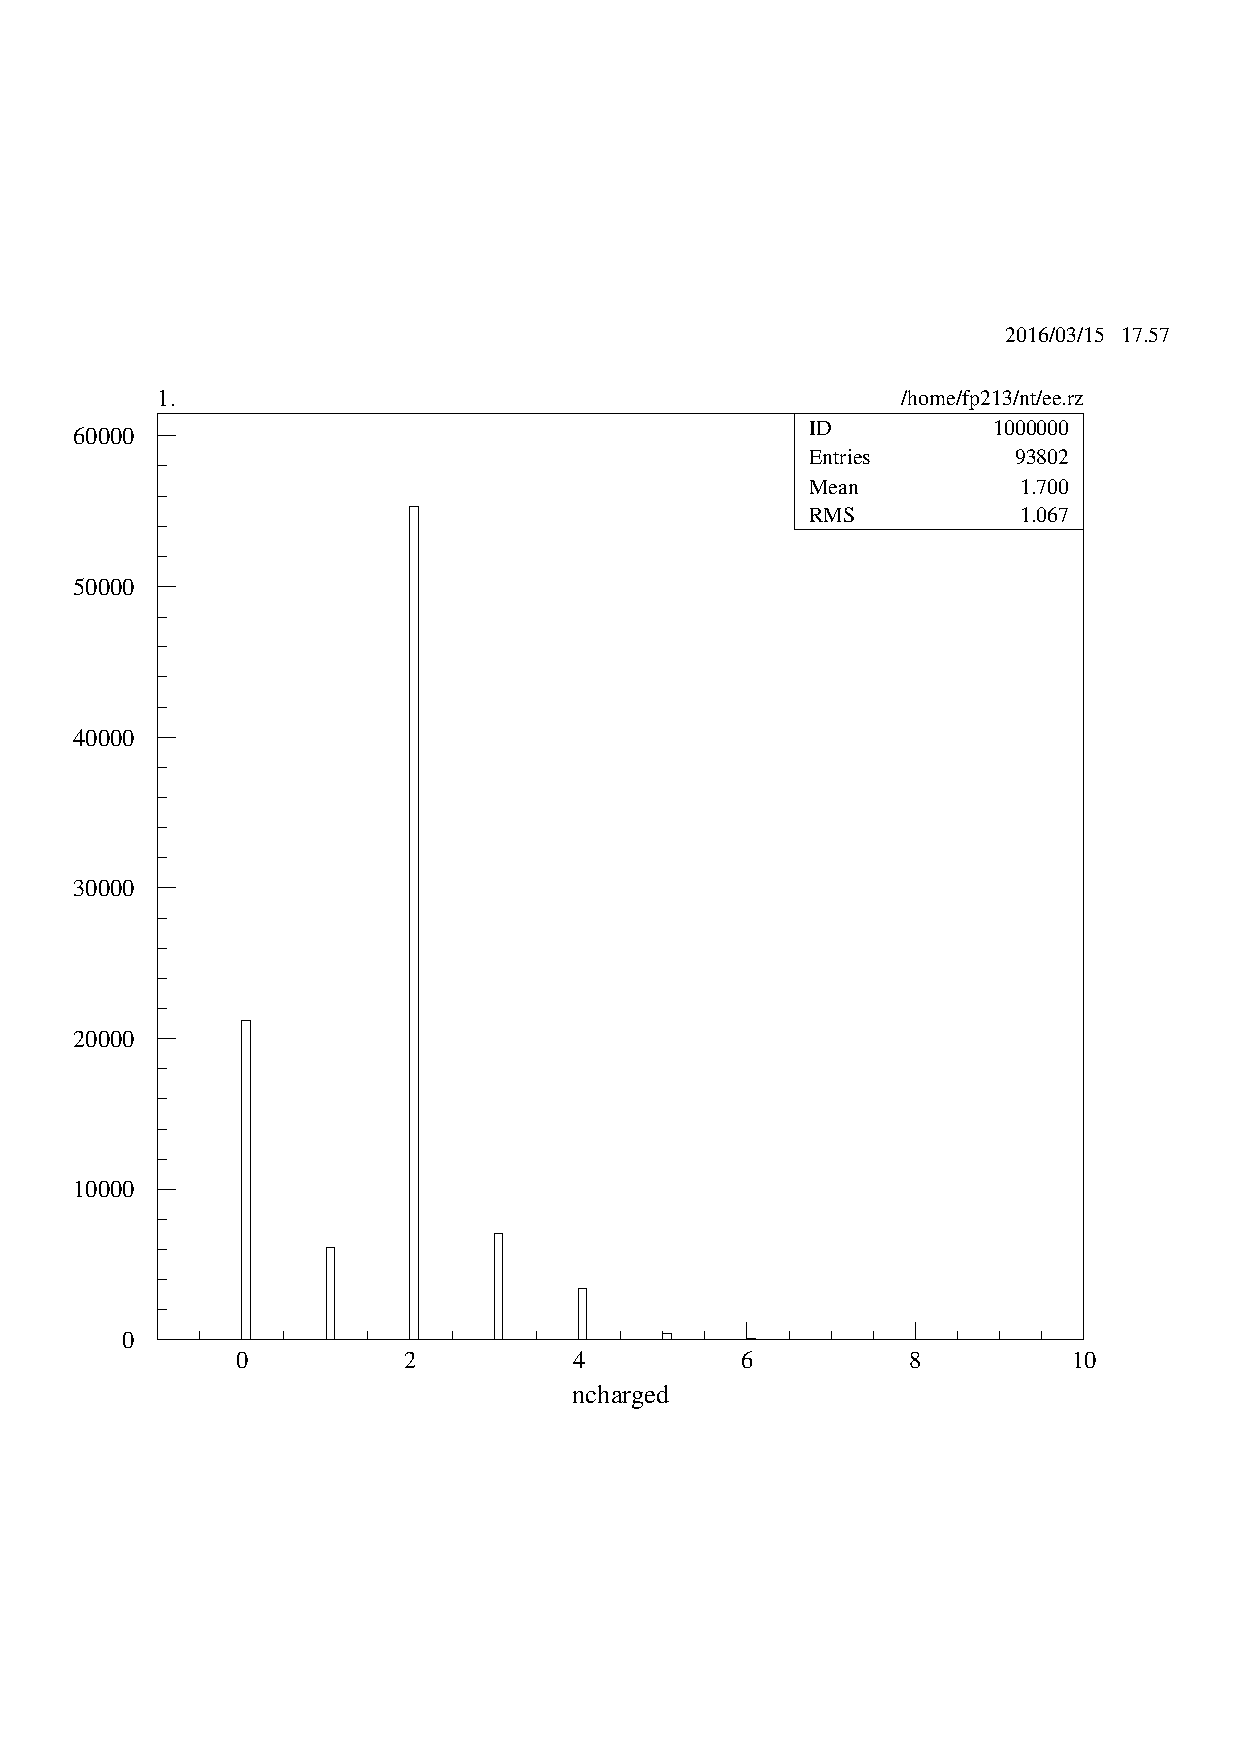
\includegraphics[width=\linewidth]{electrons-ncharged}
        \caption{%
            Electrons
        }
        \label{fig:paw-ncharged/electrons}
    \end{subfigure}
    \hfill
    \begin{subfigure}[c]{0.48\linewidth}
        \centering
        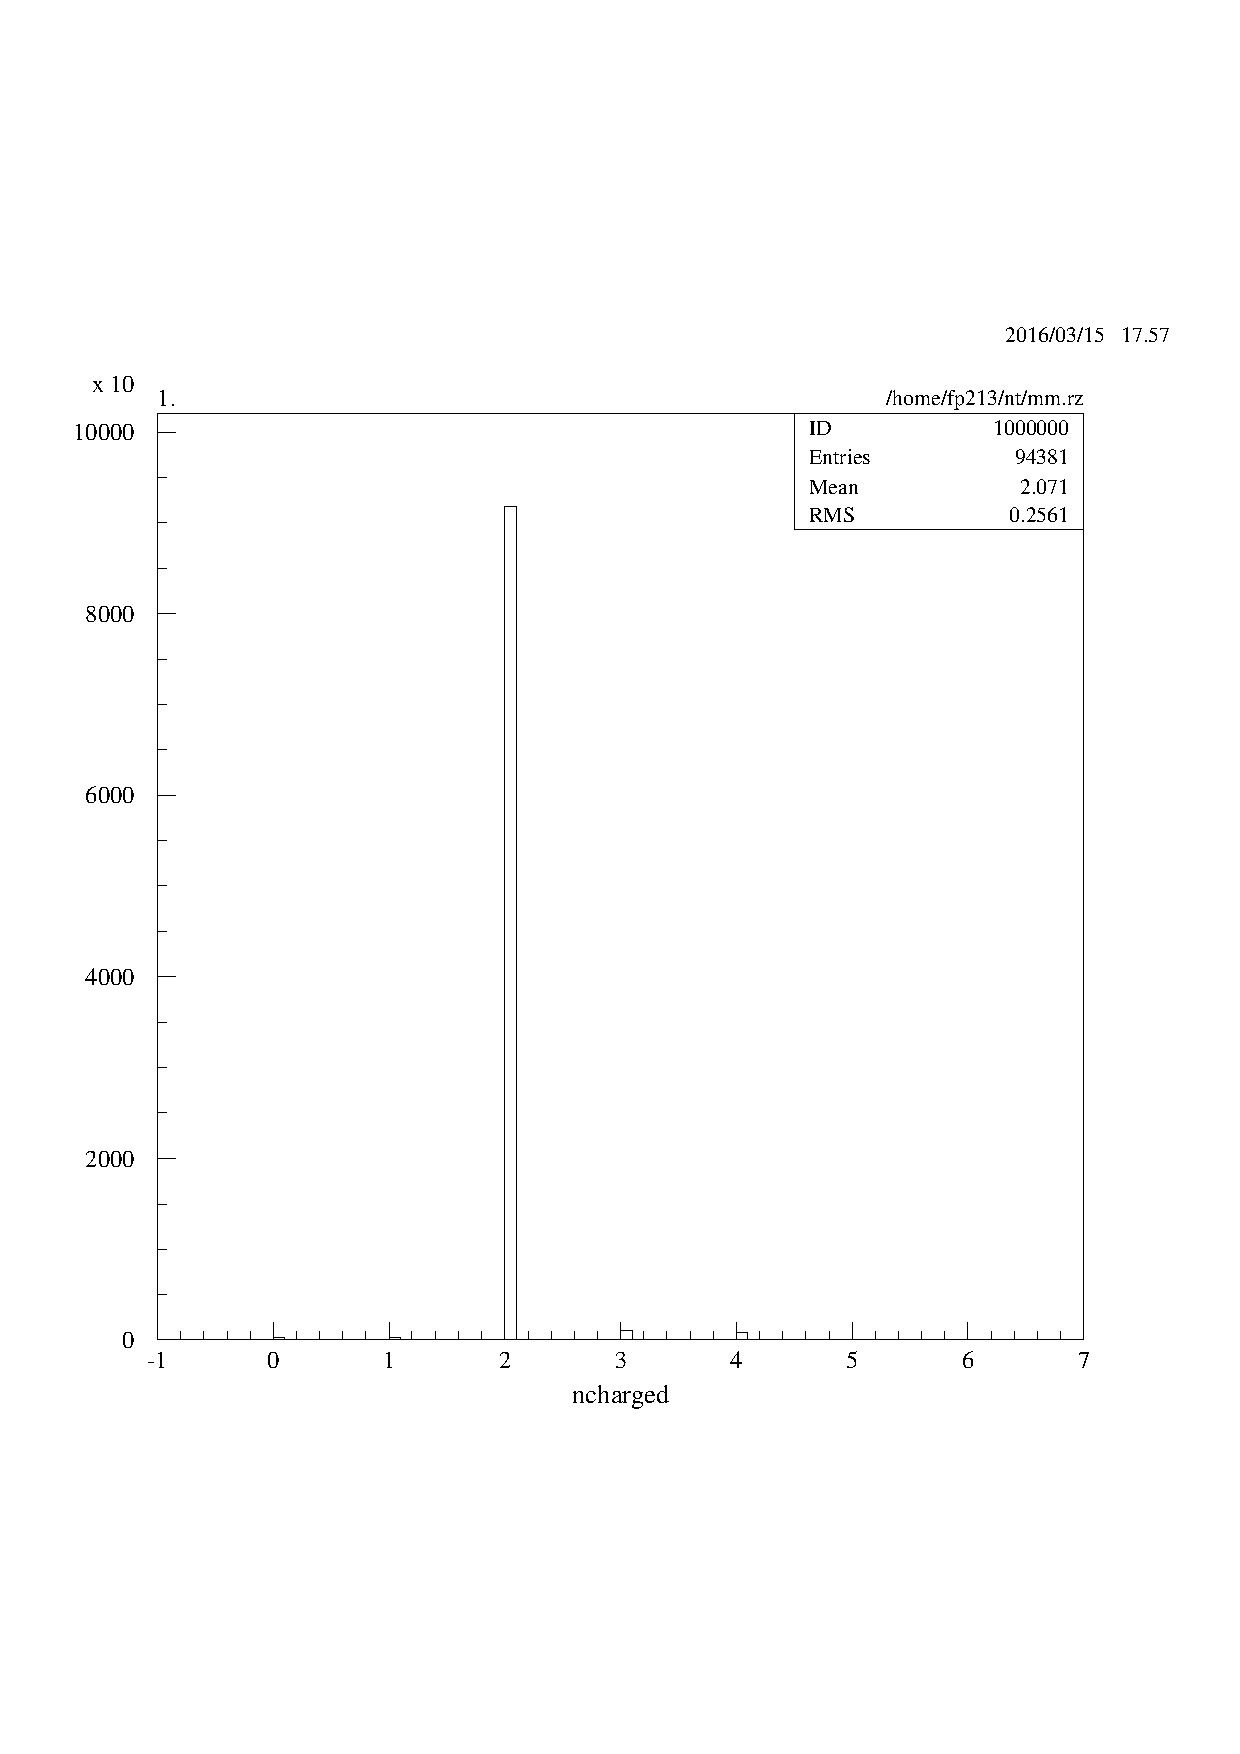
\includegraphics[width=\linewidth]{muons-ncharged}
        \caption{%
            Muons
        }
        \label{fig:paw-ncharged/muons}
    \end{subfigure}

    \vspace{2ex}

    \begin{subfigure}[c]{0.48\linewidth}
        \centering
        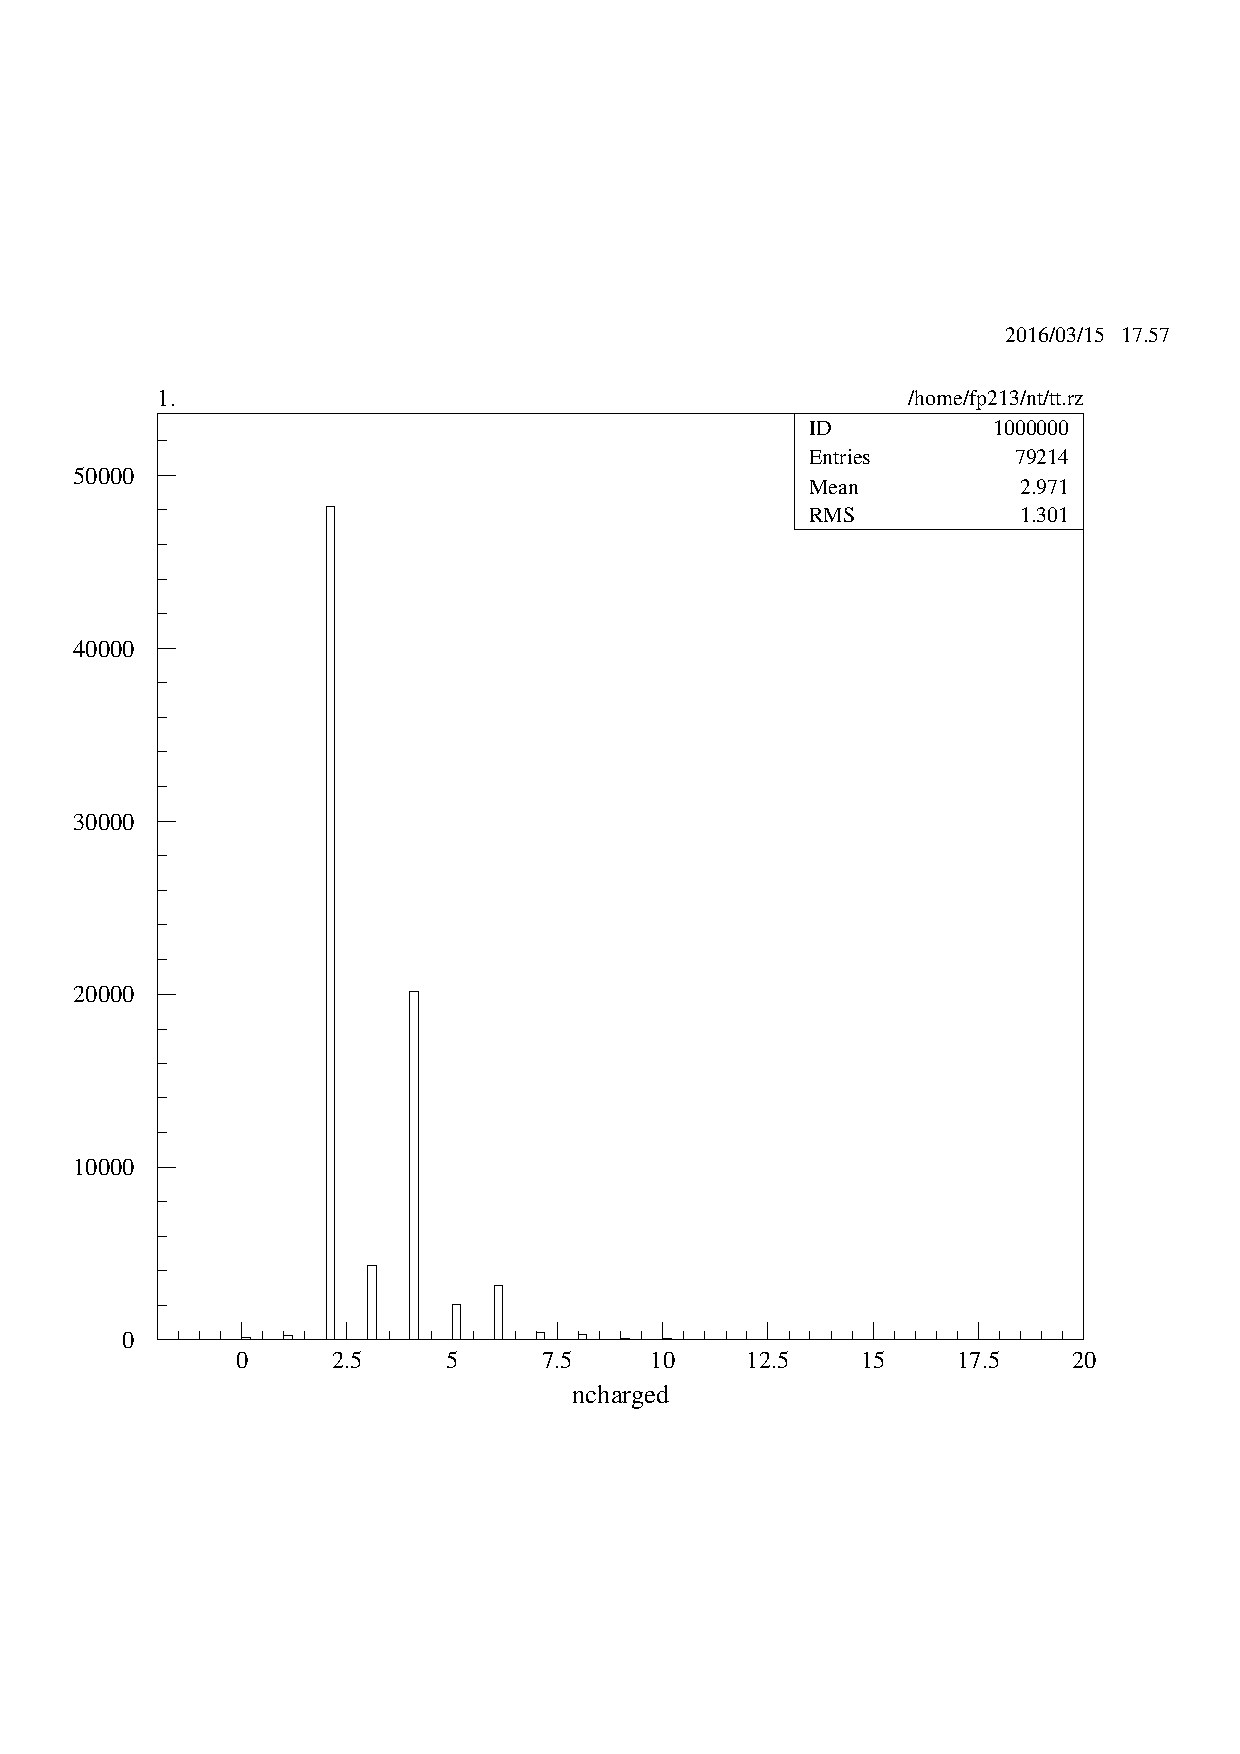
\includegraphics[width=\linewidth]{taus-ncharged}
        \caption{%
            Tauons
        }
        \label{fig:paw-ncharged/tuaons}
    \end{subfigure}
    \hfill
    \begin{subfigure}[c]{0.48\linewidth}
        \centering
        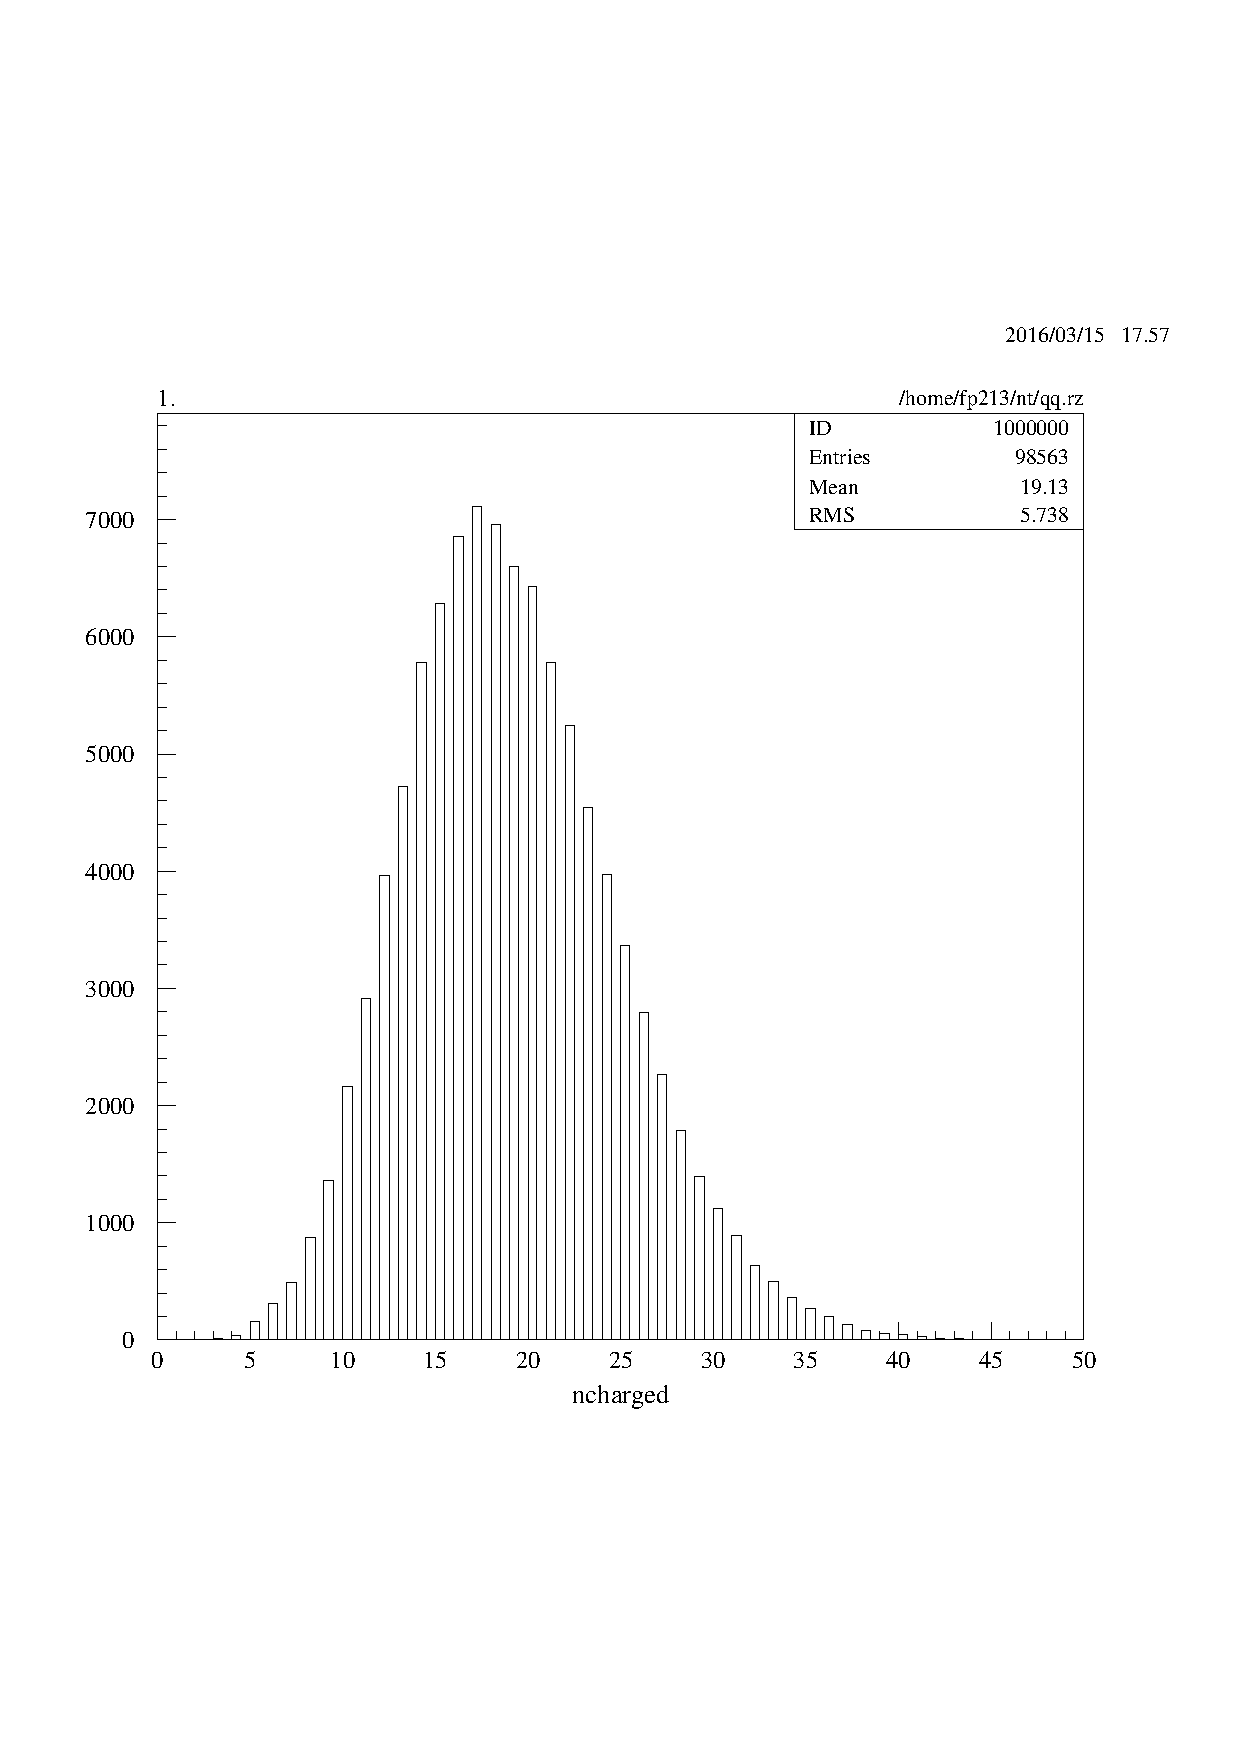
\includegraphics[width=\linewidth]{hadrons-ncharged}
        \caption{%
            Hadrons
        }
        \label{fig:paw-ncharged/hadrons}
    \end{subfigure}

    \caption{%
        Number of charged tracks, \ncharged, for the four decay types.
        Histograms generated with \textsc{paw} from Monte Carlo datasets.
    }
    \label{fig:paw-ncharged}
\end{figure}


With a magnifying glass we can see that there are mostly two charged tracks for
electron and muon decays. Interestingly, there are occasionally three to four
tracks for the electron.

As expected from decay modes with hadrons, we see that tauons can have six
charged tracks. Hadrons can also decay with six or less charged tracks, but the
most part decays with more than ten tracks.

The other characteristics were also plotted using \textsc{paw}. \pcharged\ is
shown in Figure~\ref{fig:paw-pcharged}, \eecal\ in Figure~\ref{fig:paw-e_ecal}
and \ehcal\ in Figure~\ref{fig:paw-e_hcal}.

\subsection{Angular distribution}

As one can see in Figure~\ref{fig:paw-angle}, the angular distribution of the
four decay modes is not the shifted parabola as expected from the $s$-channel
theory. For the electrons, this arises from the mixing with the $t$-channel. We
do not want to include the $t$-channel reactions as this would make a
comparison to the other leptonic channels (only $s$-channel there) impossible.

We have shown in Figure~\ref{fig:channels} how the $s$- and $t$-channel scale
with the angle. At small angle, the unwanted $t$-channel dominates. Therefore
we need to cut large $\cos(\theta)$ out of our analysis. The efficiency will do
down, but the quality of the remaining data will be better. We also cut the
peak at $\cos(\theta) < -0.9$ as we do not know its origin but know that it
cannot come from a simple $s$-channel process.


\begin{figure}
    \centering
    \begin{subfigure}[c]{0.48\linewidth}
        \centering
        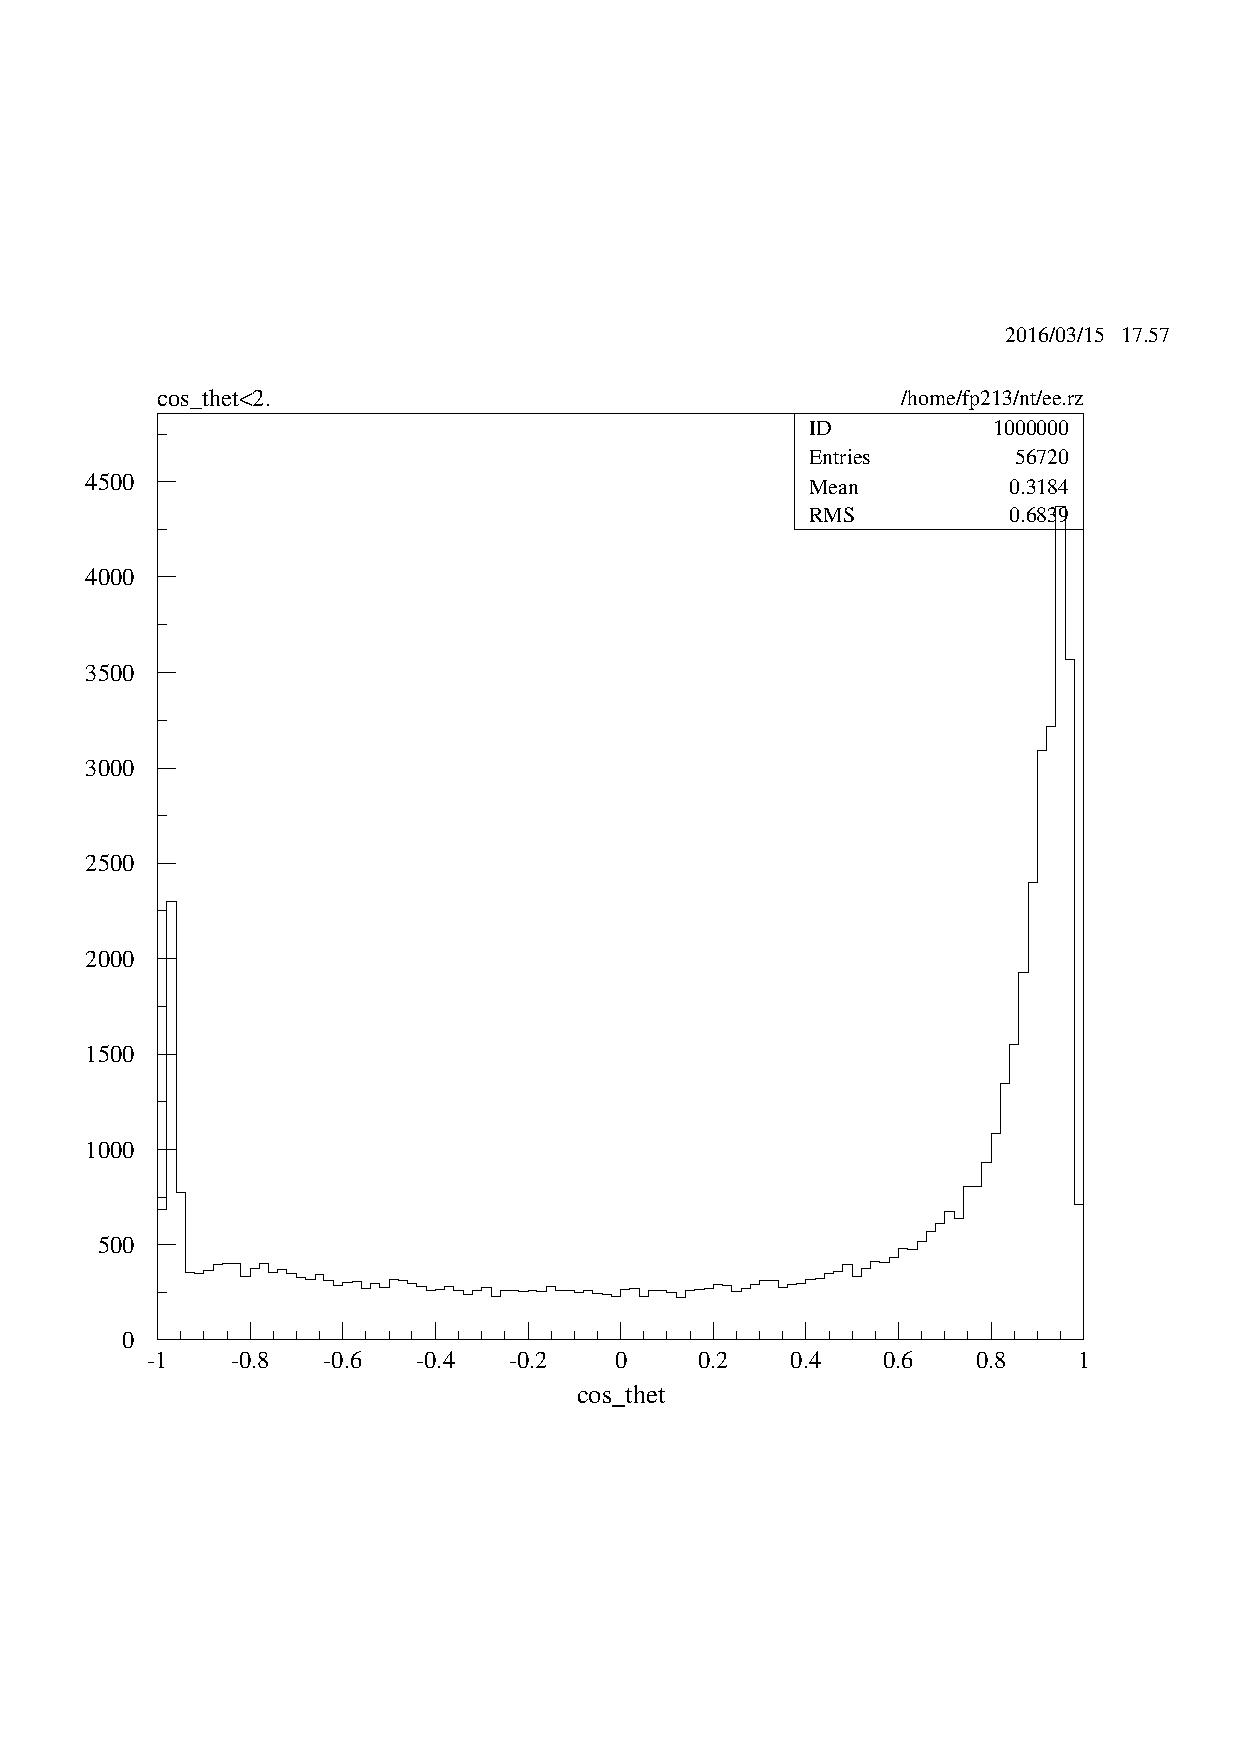
\includegraphics[width=\linewidth]{electrons-cos_thet}
        \caption{%
            Electrons
        }
        \label{fig:paw-angle/electrons}
    \end{subfigure}
    \hfill
    \begin{subfigure}[c]{0.48\linewidth}
        \centering
        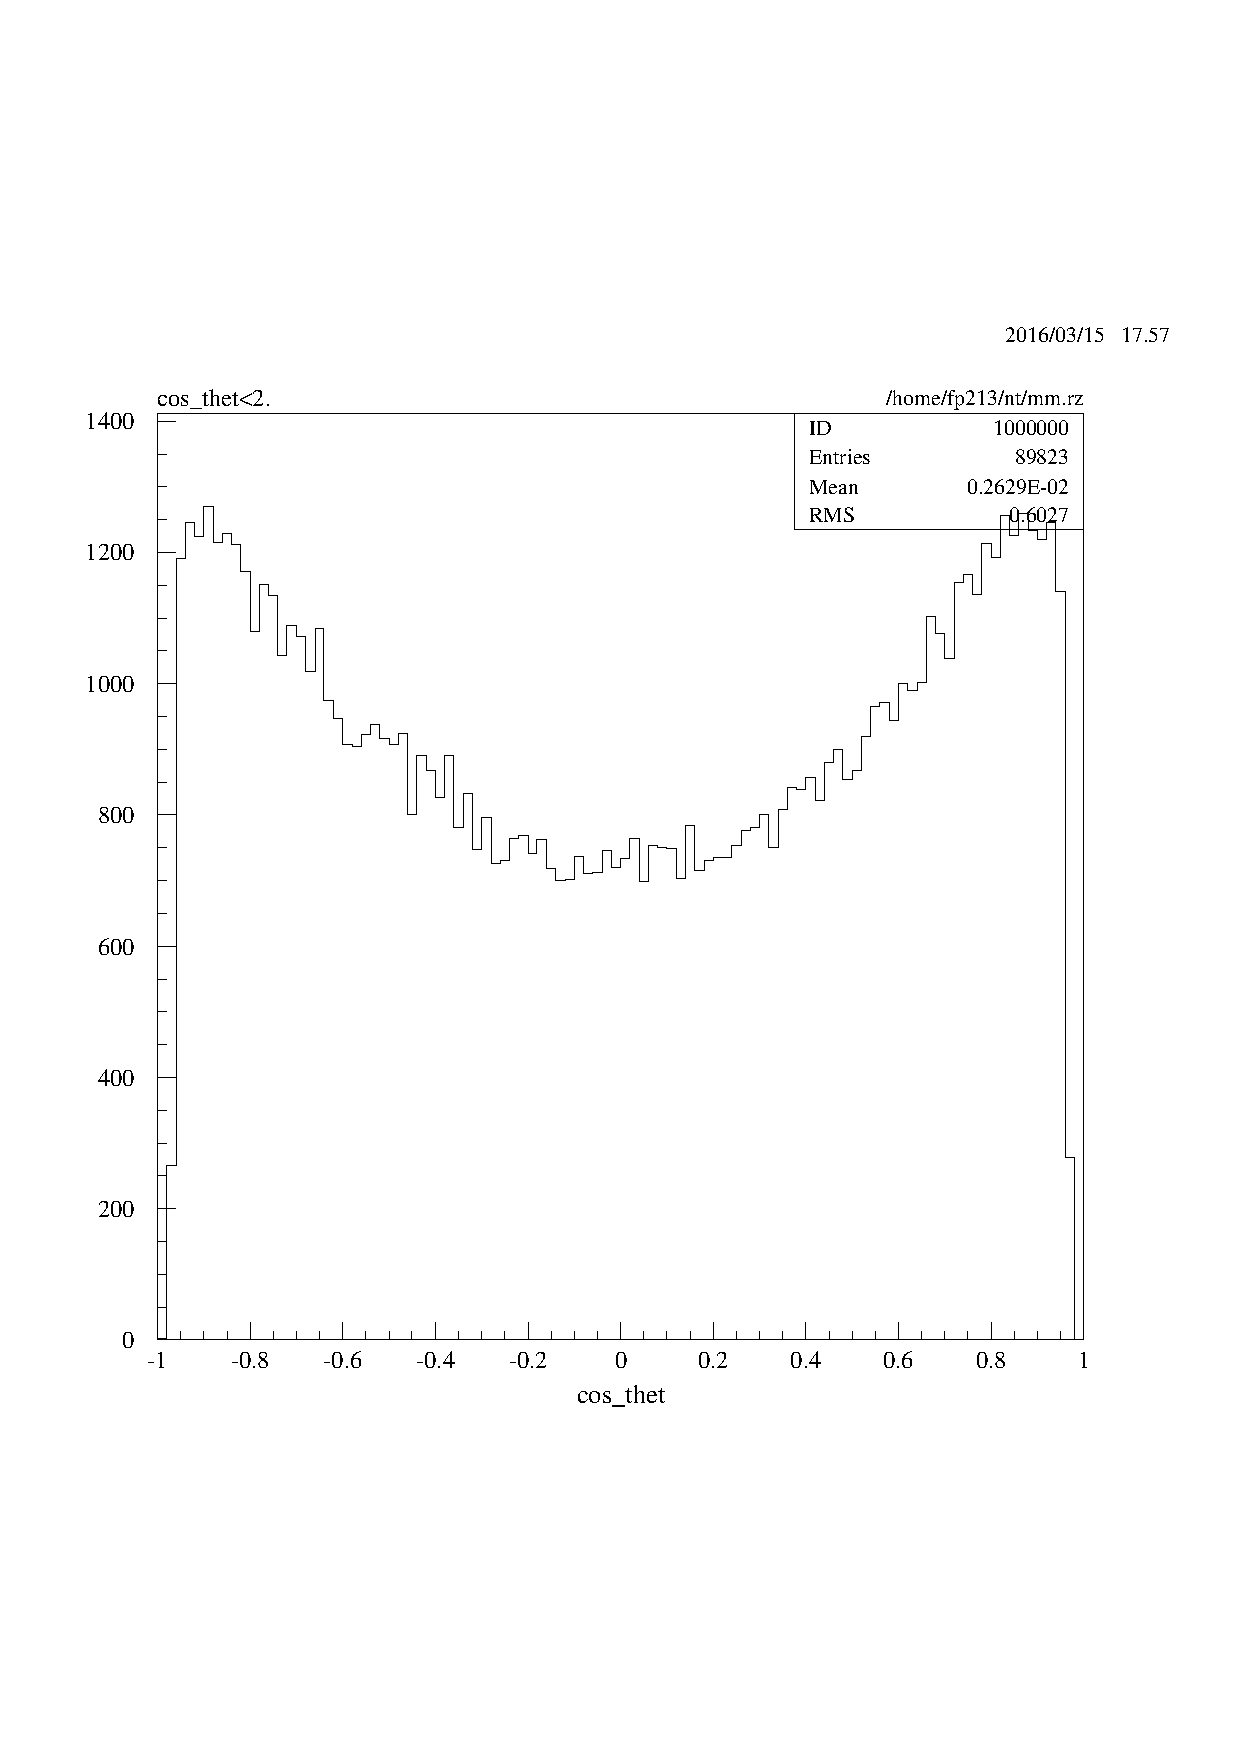
\includegraphics[width=\linewidth]{muons-cos_thet}
        \caption{%
            Muons
        }
        \label{fig:paw-angle/muons}
    \end{subfigure}

    \vspace{2ex}

    \begin{subfigure}[c]{0.48\linewidth}
        \centering
        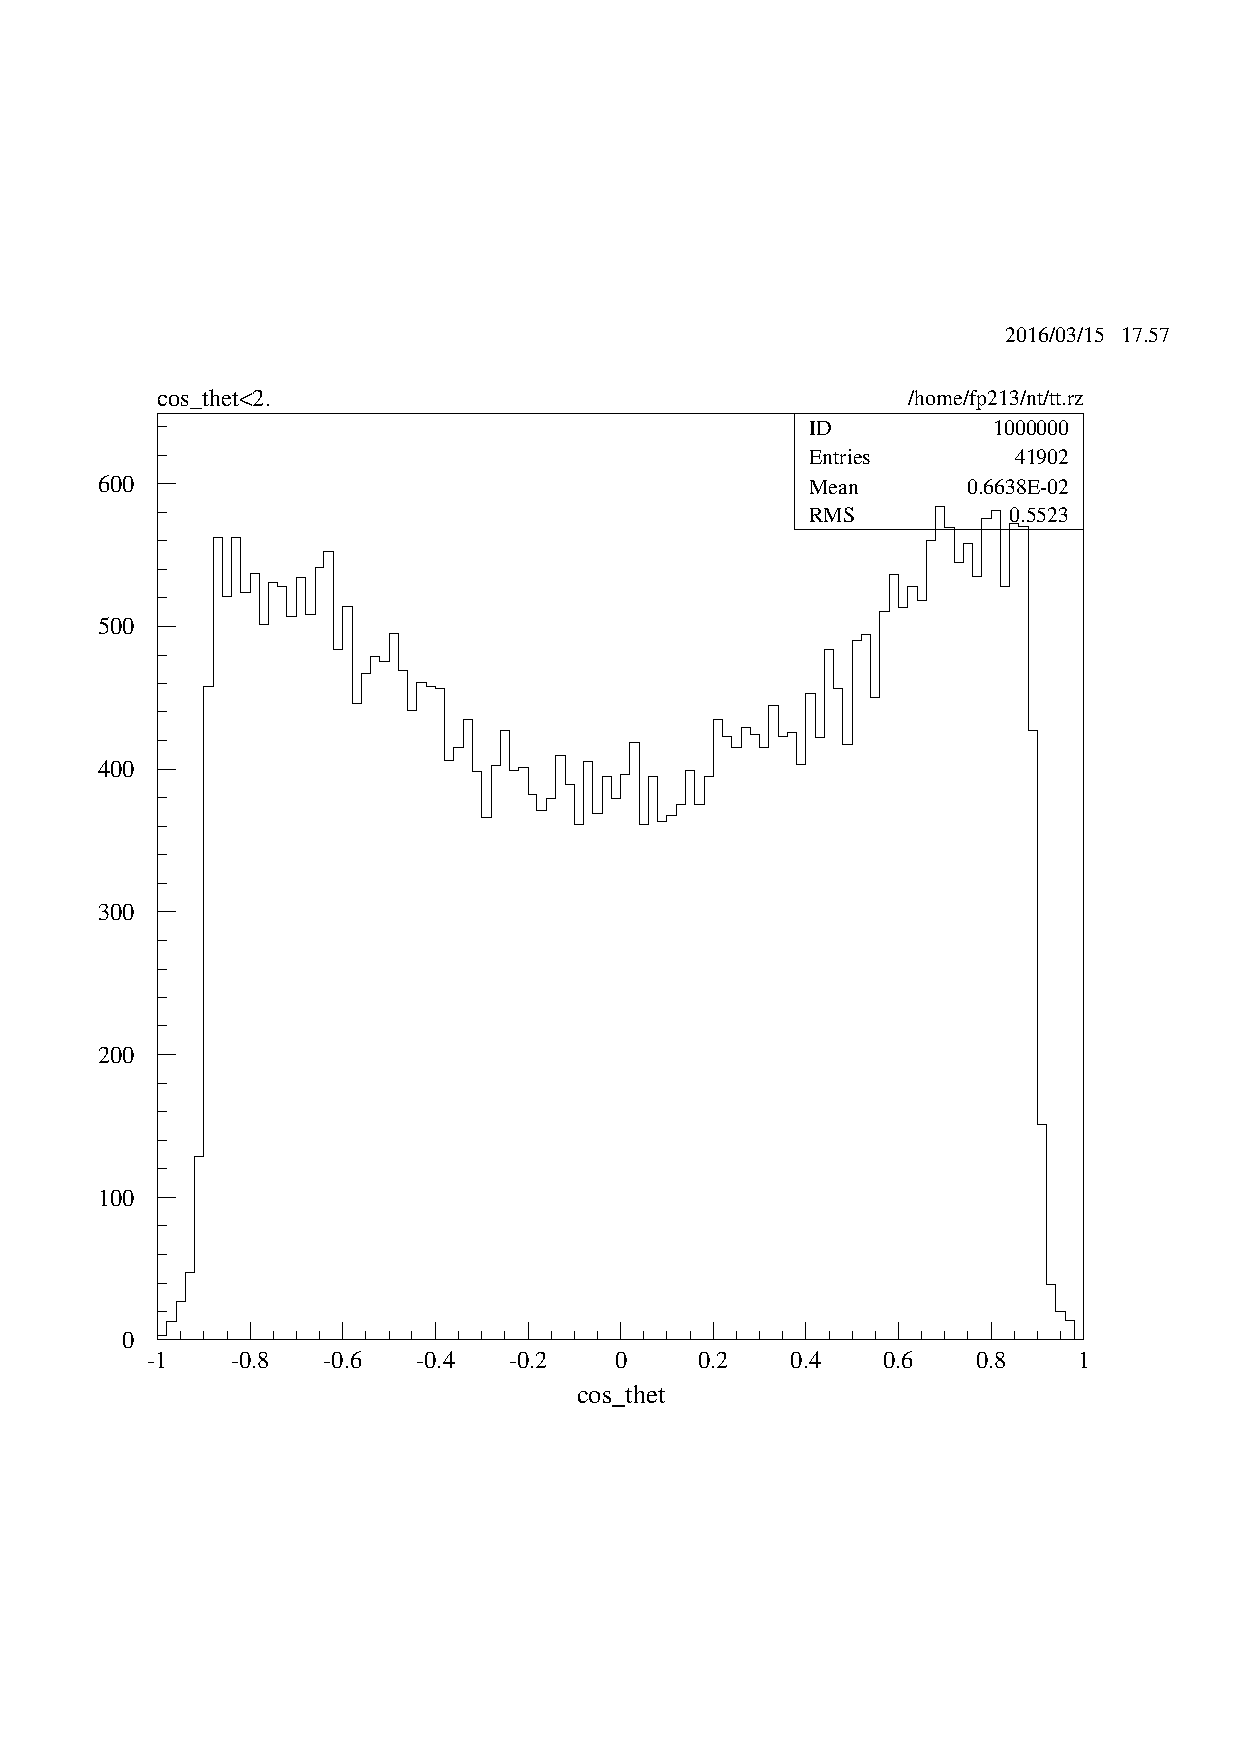
\includegraphics[width=\linewidth]{taus-cos_thet}
        \caption{%
            Tauons
        }
        \label{fig:paw-angle/tauons}
    \end{subfigure}
    \hfill
    \begin{subfigure}[c]{0.48\linewidth}
        \centering
        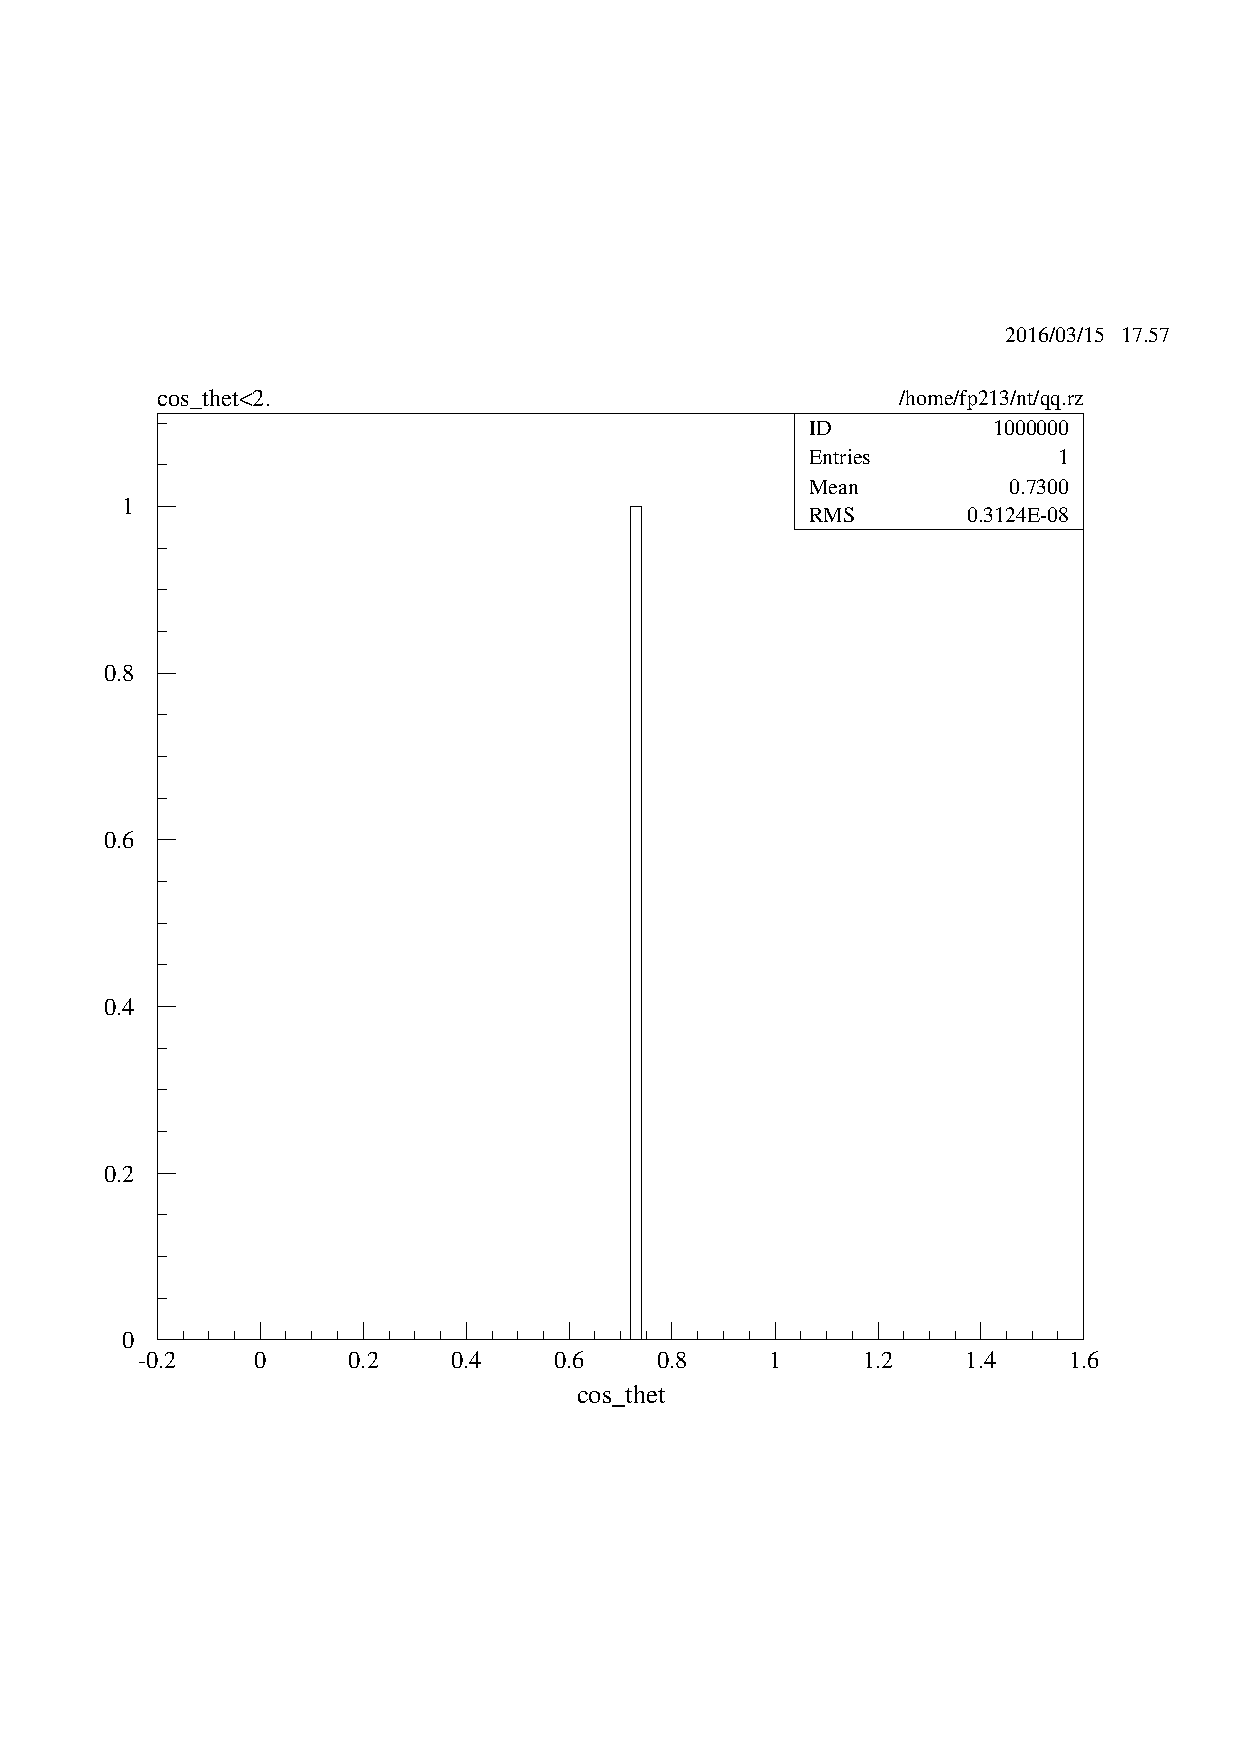
\includegraphics[width=\linewidth]{hadrons-cos_thet}
        \caption{%
            Hadrons
        }
        \label{fig:paw-angle/hadrons}
    \end{subfigure}

    \caption{%
        Angular distribution with respect to $\cos(\theta)$ for the four decay
        types. Histograms generated with \textsc{paw} from Monte Carlo
        datasets. Events without a defined angle are excluded, therefore there
        are no events with more or less than one positively charged track
        included.
    }
    \label{fig:paw-angle}
\end{figure}


The muons (see Figure~\ref{fig:paw-angle/muons}) look pretty good. At
$|\cos(\theta)| > 0.9$ we have a sharp drop which we blame on the detector not
covering the whole solid angle. Since the beam pipe needs to go through the
detector, one cannot detect collinear events. We therefore cut those events
away.

The shape of the tauons (see Figure~\ref{fig:paw-angle/tauons}) seems to be a
parabola in the middle but flatten off to the sides. Events with only one
charged positive track have to be a decay into an positron or an anti-muon. A
neutrino is created in those processes, skewing the angular distribution.
Therefore this flattening does not need to be cut out as we have a physical
explanation for it.

For the hadrons (see Figure~\ref{fig:paw-angle/hadrons}), an angular
distribution is rarely defined, there is only one event that even has a
well-defined $\theta$-angle. Therefore we do not perform any cutting in the
hadronic sector.

Our refined and final cuts including the angle are listed in
Table~\ref{tab:cuts2}.

\begin{table}
    \centering
    \begin{tabular}{lccccc}
        \toprule
        & \multicolumn{5}{c}{Cut criterion} \\
        \cmidrule(l){2-6}
        Particle
        & \ncharged
        & \pcharged/\si{\giga\electronvolt}
        & \eecal/\si{\giga\electronvolt}
        & \ehcal/\si{\giga\electronvolt}
        & $\cos(\theta)$
        \\
        \midrule
        Electrons & $< 4$ &  & $> 60$ &  & $\num{-.9}\leq\dots\leq\num{.5}$ \\
        Muons & $< 4$ & $> 75$ & $< 20$ &  & $\num{-.9}\leq\dots\leq\num{.9}$ \\
        Tauons & $< 7$ & $< 75$ & $\leq 75$ &  &\\
        Hadrons & $> 7$ &  &  &  & \\
        \bottomrule
    \end{tabular}
    \caption{%
        Cuts derived from the full Monte Carlo datasets.
    }
    \label{tab:cuts2}
\end{table}

\section{Bootstrap error estimation}

The default method for error estimation is the \emph{Gaussian error
propagation}. This works by applying $[\Deltaup f](x) = |f'(x)| \cdot \Deltaup
x$ for every transformation used. The implicit assumptions used here are that
errors are both small and Gaussian throughout the analysis. Especially if one
has a lot of analysis steps, the propagated error might be too large or small.

Besides being tedious, this scheme also does not provide any help when doing
fits. Methods like the \texttt{scipy.optimize.curve\_fit}, which we use here,
will give a covariance matrix. Taking the square root of the diagonal usually
gives a sufficient error estimate if the error are uncorrelated, which is often
the case. Although the function can perform an error-weighted fit, it does not
incorporate the uncertainty of the input data into the error of the fit
parameters (at least in older version). Still, uncertainties in categorical
variable (usually $x$) are not included in this function.

A method to alleviate all those problems is the \emph{bootstrap} method. It is
an intrinsically numerical and statistical procedure. It is a \enquote{meta
analysis of the data itself} in a sense. Instead of running our analysis once
with the original data, we also run it a couple hundred times with slightly
different datasets. This can be the same experiment conducted a couple more
times. All the input values will be slightly different according to their
statistical uncertainty. Running the analysis on all the different inputs, one
obtains a distribution of final results. Taking the standard deviation of this
distribution will be a robust estimation of the statistical error on the final
results.

As one does not have to compute partial derivatives with respect to all input
parameters, this method is very general and can be used for every step in the
analysis, even curve fitting.

Here we do not have the luxury of multiple datasets. As the detection of
particles essentially is a counting experiment, we assume that a value $N$ is
associated with a standard deviation of $\sqrt N$. We only have one data point,
so we cannot do a bootstrap right away. Therefore we draw more data points from
a Gaussian distribution centered on $N$ with width $\sqrt N$. The values that
we get should roughly be the same we would have gotten when performing the
analysis with another data set.

This method sounds outrageous, we just pull more data \enquote{out of the hat}
by doing this resampling. Gaussian error propagation does the same thing,
really, just analytically. Therefore we are performing the same procedure, just
with numerical methods and less assumptions.

Another aspect that one should cover in curve fitting is the dependence of the
result on the number of data points used. In an ideal case we can remove any of
the points and the fit would still give the same result. Later we will have
fits with seven data points and see that removing any of the points will
drastically alter the curve. In order to obtain this effect, we do a
\emph{Jackknife} in first order for the fits as well. Instead of fitting with
all seven points, we randomly remove one of the points in each run of the fit.
As we perform hundreds of bootstrap samples, the mean value will not be altered
much. The standard deviation of the fit parameters will increase, just what we
want for fragile fits. We will see this at the cross sections later on.

Usually, only one fit curve is given. The bootstrap method will also give us a
distribution of fit curves which we plot as a band of curves. Correlation
between the fit parameters will become directly visible.

Gaussian error propagation assumes that errors are symmetric around the mean
value. In realistic examples, this might not be the case. We can obtain
asymmetric errors using the percentiles of the bootstrapped distribution. This
will be seen in the forward--backward asymmetry.

\section{Muon forward--backward asymmetry}

The muon forward--backward asymmetry is a quantity that we want to extract from
the data. For this we need to filter the actual dataset (in our case number 1)
for muons. Then we also need to filter by beam energy. The dataset contains
seven different beam energies, we define seven more filters like the following:

\begin{lstlisting}
nt/cuts $11 e_lep>44.0.and.e_lep<44.5
nt/cuts $12 e_lep>44.5.and.e_lep<45.0
\end{lstlisting}

Using those, we can filter the data for muons (\texttt{\$2}), positive or
negative angle (\texttt{cos\_thet<0.} or \texttt{cos\_thet>0}) and for the energy (\texttt{\$11}). Printing this as
a histogram, we use the following code:

\begin{lstlisting}
nt/plot daten1.cos_thet $2.and.cos_thet<0..and.$11
pict/print afb-muons-daten1-negative-energy1.ps
nt/plot daten1.cos_thet $2.and.cos_thet>0..and.cos_thet<2..and.$11
pict/print afb-muons-daten1-positive-energy1.ps
\end{lstlisting}

We have also supplied the additional criterion for sensible angles
(\texttt{cos\_thet<2.}) because undefined angles have a numerical value way
greater than two.

From the exported diagrams (not included in this report) we extract the number
of events with $\cos(\theta) > 0$, which we call $N_+$, and the events with
$\cos(\theta) < 0$, which we call $N_-$. The asymmetry is then simply
\[
    A_\text{FB} = \frac{N_+ - N_-}{N_+ + N_-} \,.
\]

Our analysis to this point is based on the tree level formalism. Higher order
corrections are needed in every QFT for more accurate result. Here we are given
the combined effect of all those corrections as a table of shift for
$A_\text{FB}$. For each beam energy, we add the correction and obtain a final
value for $A_\text{FB}$. The resulting asymmetries for the different beam
energies are shown in  Table~\ref{tab:afb} and Figure~\ref{fig:plot-afb}. Error
estimation is done by assuming an error of $\sqrt{N}$ for all the counts and
using resampling bootstrap for the final result.

\begin{table}
    \centering
    \begin{tabular}{SS}
        \toprule
        {$\sqrt s$} & {$A_\mathrm{FB}$} \\
        \midrule
        %< for row in afb_table >%
        << ' & '.join(row) >> \\
        %< endfor >%
        \bottomrule
    \end{tabular}
    \caption{%
        Forward--backward asymmetry in the muon events.
    }
    \label{tab:afb}
\end{table}

\begin{figure}
    \centering
    \includegraphics{plot-afb}
    \caption{%
        Forward--backward asymmetry in the muon events. Shown are corrected
        values for $A_\text{FB}$.
    }
    \label{fig:plot-afb}
\end{figure}

The figure also includes the theoretical expectation that we have computed in
the exercises in Section~\ref{sec:exercises-asymmetry}. We have re-computed the
expectation value with the physical value of $\sin(\theta_\text w)^2$ for the
various beam energies used. Our results do not imply this exact trend (i.e.\
almost constant) of the asymmetry. However, as the errors are quite large, our
measurements are still consistent with it.

\subsection{Weak mixing angle}

At the peak, the relation
\[
    A_\text{FB}^\text{peak} \simeq 3 \del{\frac{v_\mathrm l}{a_\mathrm l}}
    \qquad\text{and}\qquad
    \frac{v_\mathrm l}{a_\mathrm l} = 1 - 4 \sin(\theta_\mathrm w)^2
\]
holds for leptons. Taken from the manual, Equation~(2.21). Using the asymmetry
value at the peak (fourth data point), we obtain $\sin(\theta_\mathrm w)^2 =
\num{<< sin_sq_afb >>}$ from
\[
    \sin(\theta_\mathrm w)^2 = \frac{1 - \sqrt{A_\text{FB}^\text{peak} / 3}}4
    \,.
\]
Due to the square root in the used relation, the bootstrap sampling can
encounter illegal values which we just drop. The ratio of ignored values is
\SI{<< sin_sq_bootstrap_acceptance >>}{\percent}, which is quite high. All
values that are used are shown in Figure~\ref{fig:afb-boot-hist}. Although this
seems bad, this only affected the error estimation. The distribution of
resulting $\sin(\theta_\mathrm w)^2$ values is shown in
Figure~\ref{fig:sin_sq-boot-hist}. One can see that is it rather symmetric but
not centered around the value we obtain by computing with the actual input (not
resampled). Therefore we conclude that we actually have a significant
asymmetric error, namely $\sin(\theta_\mathrm w)^2 = << sin_sq_afb_asym >>$.

\begin{figure}
    \centering
    \begin{subfigure}[t]{0.48\linewidth}
        \centering
        \includegraphics{afb-boot-hist}
        \caption{%
            Asymmetry values. Only the positive ones are actually taken, those
            are marked in gray.
        }
        \label{fig:afb-boot-hist}
    \end{subfigure}
    \hfill
    \begin{subfigure}[t]{0.48\linewidth}
        \centering
        \includegraphics{sin_sq-boot-hist}
        \caption{%
            Weak mixing angle. The shape is quite symmetric but not centered
            around actual value.
        }
        \label{fig:sin_sq-boot-hist}
    \end{subfigure}
    \caption{%
        Histograms of the distributions used in the bootstrap error estimation.
    }
    \label{fig:boot-hist}
\end{figure}

\section{Detection efficiency}
\label{sec:detection-efficiency}

By choosing the cuts in a particular way, we make a compromise between
detection efficiency and underground. Choosing a tight cut will discard events
that should have been counted. This will lead to a loss of a certain fraction
of events. This is not directly a problem as we can just compensate by this
loss factor. However, our statistical errors will grow as we have less
statistics. A loose cut will water the sorting with underground events. Say we
want to filter out electrons but our cuts are too loose. Then some tauon events
might slip into the electrons category.

Both types of errors, the false-negatives and the false-positives, can be
handled using a detection matrix~$\mat D$ and Monte Carlo datasets.
The Monte Carlo datasets are purely of one decay channel. Therefore we know
exactly that we only have, say, electrons. Applying our cuts to the Monte Carlo
electrons, we will see how many are actually detected as electrons. This is our
efficiency. Then we take the other three kinds (muons, tauons, hadrons) of the
Monte Carlo datasets and apply the electron cuts to it. Ideally, we should not
get any events. The ratio of other events that we falsely identify as electrons
is the underground.

Using a linear model for this, we need a mapping from the actual events vector
$\vec A$ (in electron-muon-tauon-hadrons space, $\N^4$) to the identified events
vector $\vec I$ (same space). The detection matrix is then defined via $\vec I
= \mat D \vec A$. In order to find the sixteen matrix elements, we apply four
four-vector with Monte Carlo events, one for each decay type.

\subsection{Determining matrix elements}

In order to do this with \textsc{paw}, we define our final cuts for electrons,
muons, tauons and hadrons:

\begin{lstlisting}
nt/cuts $1 ncharged<4.and.e_ecal>60.and.cos_thet<.5.and.cos_thet>-0.9
nt/cuts $2 pcharged>75.and.ncharged<4.and.e_ecal<20.and.cos_thet<.9.and.cos_thet>-0.9
nt/cuts $3 pcharged<75.and.ncharged<7.and.e_ecal<75
nt/cuts $4 ncharged>7
\end{lstlisting}

We need to count the number of events that matched a given cut. Creating a
histogram with respect to an arbitrary characteristic will give us this number
as a side effect. The following generates a histogram with electron data and
the electron filter:

\begin{lstlisting}
nt/plot electrons.ncharged $1
pict/print matrix-electrons-with-electron-filter.ps
\end{lstlisting}

And this generates a histogram with muon data and the same filter:

\begin{lstlisting}
nt/plot muons.ncharged $1
pict/print matrix-muons-with-electron-filter.ps
\end{lstlisting}

Similar expressions are needed for the other matrix element, in total we need
16 of those counting histograms. The resulting histograms are shown in
Figure~\ref{fig:paw-matrix-electrons}. Squint at the row \enquote{Entries} in
the legend, this is the interesting number.

For the electrons, the Monte Carlo input vector is $\vec A = (94381, 0, 0,
0)^\mathrm T$. Then we look at the output in the four histograms and find $\vec
I = (20474, 1, 1013, 0)^\mathrm T$. From this, we can construct the first
column in the matrix. Using the other filters, we can construct the whole
matrix. Table~\ref{tab:matrix} shows the matrix. It can be seen that it is
mostly diagonal, just as we want it to be. The detection efficiency for the
electrons is not very great. This comes from the severe cutting in
$\cos(\theta) < 0.5$ which discards a lot of events.

\begin{table}
    \centering
    \begin{tabular}{lSSSS}
        \toprule
        & \multicolumn{4}{c}{Acceptance rate / \si{\percent}} \\
        \cmidrule(l){2-5}
        {Detected as}
        & {Electrons}
        & {Muons}
        & {Tauons}
        & {Hadrons} \\
        \midrule
        %< for row in matrix >%
        << ' & '.join(row) >> \\
        %< endfor >%
        \bottomrule
    \end{tabular}
    \caption{%
        The detection matrix $\mat D$. Although it is displayed in a table, it
        is meant as a matrix which can be right-multiplied with an actual
        events vector $\vec A$. The resulting vector will be the vector of
        identified events $\vec I$ of our cuts. The matrix is mostly diagonal,
        the low number for electron--electron is due to our mistake in angular
        restriction (see text).
    }
    \label{tab:matrix}
\end{table}

The errors given in the matrix are the assumed $\sqrt N$ standard deviation
from a counting experiment.

\subsection{Inverting the matrix}

We need to invert the matrix in order to use this detection matrix~$\mat E$ as
a correction. This will be numerically stable as it is almost diagonal. The
inverted matrix is shown in Table~\ref{tab:inverted}. The errors for the matrix
elements come directly from the bootstrapping.

\begin{table}
    \centering
    \begin{tabular}{lllll}
        \toprule
        & \multicolumn{4}{c}{Correction factor} \\
        \cmidrule(l){2-5}
        {Actually are}
        & {Electrons}
        & {Muons}
        & {Tauons}
        & {Hadrons} \\
        \midrule
        %< for row in inverted >%
        << ' & '.join(row) >> \\
        %< endfor >%
        \bottomrule
    \end{tabular}
    \caption{%
        The inverted detection matrix $\mat D\inv$.
    }
    \label{tab:inverted}
\end{table}

\subsection{Conceptual mistake}

There is one mistake that we did in the derivation of the matrix, and we cannot
recover from this after the fact. The matrix was set up using the final cuts,
which also means that we only allow $\cos(\theta) \leq \num{0.5}$ in the
electrons. We did that to filter out the $t$-channel. As one can see in the
inverse detection matrix in Table~\ref{tab:inverted}, the correction factor for
the electron--electron case is around \num{4.6}. This is way larger than the
other diagonal elements. The matrix element is this large as we have made a
severe cut and filtered out most of the electron events. In contrast to the
other channels, this is something we actually want in order to get rid of the
$t$-channel!

Using the matrix $\mat D\inv$ now, the $t$-channel will come back, at least
from the numbers. Therefore we will find later on that the cross sections of
the scattering into electrons. Table~\ref{tab:cross-sections} and
Figure~\ref{fig:cross-sections} clearly show this apparent violation of lepton
universality.

This is an overcompensation in our correction, we should have also cut the
Monte Carlo data in the angle. The Monte Carlo data contains $t$-channel events
as well, which we also do not want. By taking the ratio of filtered electrons
and unfiltered Monte Carlo electrons, our acceptance ratio will correct the
$t$-channel back in. We should actually have filtered the Monte Carlo with the
same $\cos(\theta) \leq \num{0.5}$ cut in order to have a reduced number of
false-negatives and therefore no overcompensation. We do not have access to the
machines running \textsc{paw} now, so we can just explain why the results do
not come out right and use the values for the muons as an replacement,
\emph{assuming} that lepton universality does hold.

\section{Partial cross sections}

\subsection{Counts}

In order to compute cross sections, we need count rates. We have filtered the
dataset with our cuts and an energy selection. For instance in the following
snippet we use the muon filter (\texttt{\$2}) with the third beam energy
(\texttt{\$13}):

\begin{lstlisting}
nt/plot daten1.ncharged $2.and.$13
pict/print filtered-daten1-as-muon-energy3.ps
\end{lstlisting}

We look at the generated histograms and extract the number of events from each
histogram. The results are collected in Table~\ref{tab:counts}. Shown are the
errors which we assume to be $\sqrt{N}$ as this is a counting experiment. Those
errors are also used for resampling.

\begin{table}
    \centering
    \begin{tabular}{SSSSS}
        \toprule
        & \multicolumn{4}{c}{Raw count} \\
        \cmidrule(l){2-5}
        {$\sqrt s / \si{\giga\electronvolt}$}
        & {Electrons}
        & {Muons}
        & {Tauons}
        & {Hadrons} \\
        \midrule
        %< for row in counts_table >%
        << ' & '.join(row) >> \\
        %< endfor >%
        \bottomrule
    \end{tabular}
    \caption{%
        Raw counts for the four decay types and seven beam energies.
    }
    \label{tab:counts}
\end{table}

The counts are just the ones left after applying the cuts. As argued in
regarding the detection efficiency (c.f.\
Section~\ref{sec:detection-efficiency}), those counts include some number of
false-positives (underground) and false-negatives (inefficiency). Therefore we
need to correct for that with the inverse matrix derived above.

Taking the four counts at each beam energy as an \enquote{identified events}
vector $\vec I$, we can use $\mat D\inv$ to give us the \enquote{actual events}
vector $\vec A$. We do this for each of the seven beam energies and obtain the
corrected counts. Those are shown in Table~\ref{tab:corrected-counts}. Again,
we have overcompensated the correction for the electrons.

\begin{table}
    \centering
    \begin{tabular}{SSSSS}
        \toprule
        & \multicolumn{4}{c}{Corrected count} \\
        \cmidrule(l){2-5}
        {$\sqrt s / \si{\giga\electronvolt}$}
        & {Electrons}
        & {Muons}
        & {Tauons}
        & {Hadrons} \\
        \midrule
        %< for row in corrected_counts_table ->%
        << ' & '.join(row) >> \\
        %< endfor ->%
        \bottomrule
    \end{tabular}
    \caption{%
        Corrected counts for the four decay types and seven beam energies.
    }
    \label{tab:corrected-counts}
\end{table}

\subsection{Incorporating the luminosity}

We want to compute the partial cross sections, those are the cross sections of
the individual decay channels. For this we just need to take the number of
counts in each channel and divide by the integrated luminosity. Therefore we
have
\[
    \sigma_i = \frac{N_i}{\int \dif t \, \mathcal L} \,.
\]

Table~\ref{tab:luminosities} lists the integrated luminosities for our dataset
taken from the manual. As the luminosities also have an error associated with
them, we will resample them as well in order to incorporate the error in our
results.

\begin{table}
    \centering
    \begin{tabular}{SS}
        \toprule
        {$\sqrt s / \si{\giga\electronvolt}$}
        & {$\int \dif t \, \mathcal L / \si{\per\nano\barn}$} \\
        \midrule
        %< for row in luminosities_table >%
        << ' & '.join(row) >> \\
        %< endfor >%
        \bottomrule
    \end{tabular}
    \caption{%
        Integrated luminosities $\int \dif t \, \mathcal L$ for the seven beam
        energies. The values are taken from the experiment description, the
        error is the total error (combined statistical and systematic error).
    }
    \label{tab:luminosities}
\end{table}

\subsection{Cross sections}

Using the relation between the counts and luminosity, we can compute the
partial cross section for each of the channels. The obtained cross sections
need to be corrected by higher-order effects. Those are given to use as simple
correction numbers, reproduced in Table~\ref{tab:radiative_cs_table}. The
results are shown in Table~\ref{tab:cross-sections}. Errors are the combined
errors of luminosity, counts and matrix elements via the bootstrap method.

\begin{table}
    \centering
    \begin{tabular}{SSSSS}
        \toprule
        & \multicolumn{2}{c}{$\Delta\sigma / \si{\nano\barn}$} \\
        \cmidrule(l){2-3}
        {$\sqrt s / \si{\giga\electronvolt}$}
        & {Hadrons}
        & {Leptons} \\
        \midrule
        %< for row in radiative_cs_table >%
        << ' & '.join(row) >> \\
        %< endfor >%
        \bottomrule
    \end{tabular}
    \caption{%
        Radiative corrections for the cross sections as given in Table~5.5 from
        the manual.
    }
    \label{tab:radiative_cs_table}
\end{table}

\begin{table}
    \centering
    \begin{tabular}{SSSSS}
        \toprule
        & \multicolumn{4}{c}{$\sigma_i / \si{\nano\barn}$} \\
        \cmidrule(l){2-5}
        {$\sqrt s / \si{\giga\electronvolt}$}
        & {Electrons}
        & {Muons}
        & {Tauons}
        & {Hadrons} \\
        \midrule
        %< for row in cross_sections_table >%
        << ' & '.join(row) >> \\
        %< endfor >%
        \bottomrule
    \end{tabular}
    \caption{%
        Cross sections for the four decay types and seven beam energies.
    }
    \label{tab:cross-sections}
\end{table}

One can already see that for the central energies around $\MZ$, the electron
cross section is too large compared to the muons and tauons. This is due to our
mistake in determining the electron matrix elements.

A graphical representation of the cross sections is shown in
Figure~\ref{fig:cross-sections}. As the individual channels have very different
height, the four channels are shown separately in
Figure~\ref{fig:cross-sections-zoom}. The figures already feature the fitted
function which we will turn to next.

\begin{figure}
    \centering
    \includegraphics{cross-sections}
    \caption{%
        Partial cross sections for each type of final state. One can see that
        the muon and tauon cross sections are similar, as expected. As we
        incorrectly correct for a $t$-channel, the electron cross section is
        too large.
    }
    \label{fig:cross-sections}
\end{figure}

\definecolor{four1}{rgb}{0.21568627450980393,0.49411764705882355,0.7215686274509804}
\definecolor{four2}{rgb}{0.596078431372549,0.3058823529411765,0.6392156862745098}
\definecolor{four3}{rgb}{0.30196078431372547,0.6862745098039216,0.2901960784313726}
\definecolor{four4}{rgb}{0.8941176470588236,0.10196078431372549,0.10980392156862745}


\begin{tikzpicture}
    \begin{axis}[
            width=\linewidth,
            height=0.6\linewidth,
            xlabel={CMS Energy $\sqrt{s} / \si{\giga\electronvolt}$},
            ylabel={$\sigma_i / \si{\nano\barn}$},
            grid=major,
            legend pos=north west,
            mymarker/.style={
                mark=+,
                only marks,
                error bars/y dir=both,
                error bars/y explicit,
            },
            band/.style={
                draw=none,
                opacity=0.3,
            },
        ]

        \addplot[
            electrons,
            mymarker,
        ] table[y error index=2] {../xy/cross_section-electrons.tsv};
        \addlegendentry{Electrons}

        \addplot[
            muons,
            mymarker,
        ] table[y error index=2] {../xy/cross_section-muons.tsv};
        \addlegendentry{Muons}

        \addplot[
            taus,
            mymarker,
        ] table[y error index=2] {../xy/cross_section-taus.tsv};
        \addlegendentry{Tauons}

        \addplot[
            hadrons,
            mymarker,
        ] table[y error index=2] {../xy/cross_section-hadrons.tsv};
        \addlegendentry{Hadrons}

        \addplot [band, fill=electrons] table {../xy/cross_section-electrons-band.tsv} \closedcycle;
        \addplot [band, fill=muons] table {../xy/cross_section-muons-band.tsv} \closedcycle;
        \addplot [band, fill=taus] table {../xy/cross_section-taus-band.tsv} \closedcycle;
        \addplot [band, fill=hadrons] table {../xy/cross_section-hadrons-band.tsv} \closedcycle;


    \end{axis}
\end{tikzpicture}


\section{Decay widths}

\subsection{Curve fitting}

From the energy dependence of the cross sections, we can compute the decay
width and the rest mass of the $\mathrm Z^0$ gauge boson generated by the
spontaneous symmetry breaking of the Higgs field. As the tree-level cross
section contains the modulus squared of the propagator, the expected energy
dependence is similar to that of a Lorentz curve,
\[
    \sigma_f \propto \frac{1}{\MZ^2} \frac{s}{(s - \MZ^2)^2 + (s^2
    \Gamma_\mathrm Z^2 / \MZ^2)} \,,
\]
taken from Equation~(3.12) in the manual. We fit a curve to the partial cross
sections for each decay channel. Luckily it is not 1992 any more and we can
just do this ourselves at home.

As we use a bootstrap scheme for error calculation, we perform the fit a couple
hundred times with resampled input data. This gives us a set of hundreds of
different fit parameters and also fit curves. For each interpolation value of
$\sqrt s$ in the resulting curve we take mean and standard deviation.
The result is shown as an error band for each fit curve.

Additionally, we have the problem that we are limited to seven beam energies.
This introduces another source of error that we control with a jackknife
approach in the fitting. Instead of fitting all seven data points, we randomly
leave one of them out and fit only the remaining six. This makes the fit still
able to converge but simulates the effect that adding or removing another data
point has. If a result changes when a single data point is removed, this should
add to the uncertainty of the result. Our fit parameters, the mass and width of
the Z-boson as well as the peak cross section, are shown in
Table~\ref{tab:lorentz-fits}.

\begin{table}
    \centering
    \begin{tabular}{lSSS}
        \toprule
        Type
        & {$\MZ / \si{\giga\electronvolt}$}
        & {$\Gamma_\mathrm Z / \si{\giga\electronvolt}$}
        & {$\sigma_f^\text{Peak} / \si{\nano\barn}$} \\
        \midrule
        %< for row in lorentz_fits_table >%
        << ' & '.join(row) >> \\
        %< endfor >%
        \bottomrule
    \end{tabular}
    \caption{%
        Fit parameters of the curves used in Figure~\ref{fig:cross-sections}
        for the partial cross sections.
    }
    \label{tab:lorentz-fits}
\end{table}

As one can see in Figure~\ref{fig:cross-sections-zoom/tauons}, the three points
in the low $\sqrt s$ area contribute a lot to the uncertainty of the fit. The
jackknife method was dearly needed, as the error in width would have been
underestimated by an order of magnitude.

\subsection{Ratios of cross sections}

The cross sections are proportional decay widths and proportional to branching
ratios. From the ratios of cross sections we can derive the ratios of branching
ratios. The decays withs are also proportional to the other quantities,
therefore we can use the theoretical decay widths to compute the expected
ratios.

From the manual we obtain the theoretical hadronic width of
\SI{1732}{\mega\electronvolt}. The leptonic width should be
\SI{83.8}{\mega\electronvolt}. Therefore we expect a ratio between the hadron
and each leptonic channel to be \num{<< br_theory >>}.

Using the values given in Table~\ref{tab:lorentz-fits}, we obtain a value of
\numlist{<< ';'.join(brs) >>} for electrons, muons and tauons, respectively.
The values for muons and tauons is in agreement with theory. The one for the
electrons is too small, which comes from the wrong analysis of the $t$-channel.

\subsection{Confidence level}

Least-squares fitting is the maximization of the likelihood function.
The minimization of the $\chi^2$ quantity with respect to the fit
parameter vector $\vec \lambda$ is an equivalent problem. The $\chi^2$ is
computed with a model $f$ and parameters $\vec\lambda$ from observations
$\{x_i\}$ using
\[
    \chi^2 = \sum_i \del{\frac{x_i - f(x_i, \vec\lambda)}{\sigma_i}}^2 \,.
\]
The fitting algorithm has already found the parameters $\vec\lambda$ (including
mass and width) for us. Now we need to compute the $\chi^2$ from this. The four
decay channels have a $\chi^2$ each of \numlist{<< ';'.join(chi_sq) >>}.

This value without the degrees of freedom is rather worthless. Therefore we
look at the \enquote{reduced $\chi^2$} which is $\chi^2/\text{dof}$. This
quantity pictorially is the average distance of the points to the curve
measured in the individual standard deviations. A value of 1 to 1.5 means that
on average, the points tangent the line with the error bar. This means that the
errors are not too large or small, the model fits. If the value is way smaller
than 1, the errors have been overestimated. If the value is larger than 1.5,
the model does not fit; points lie very far away from the curve.

Here we have seven beam energies and three model parameters, this gives
$\text{dof} = 7 - 1 - 3 = 3$. The reduced $\chi^2$ are then \numlist{<<
';'.join(chi_sq_red) >>}. Most values are quite large.

The so-called $p$-value gives the probability that the underlying model would
produce this data or a more extreme variant of this. Therefore we want a high
$p$-value, saying that the values that we have are quite normal for this model.
A common lower bound is 0.05, everything below that will reject the model.

The $p$-value is computed from the $\chi^2$ cumulative density function which
is implemented as \texttt{scipy.stats.chi2.cdf}. Inserting our values for
$\chi^2$ and $\text{dof}$, we obtain the $p$-values \numlist{<< ';'.join(p)
>>}.

All values are collected in Table~\ref{tab:confidence}. From the $p$-value we
must conclude that the Breit-Wigner prescription alone is not a good
description of the decays into muons and tauons when using the 0.05 threshold.
For the tauons, Figure~\ref{fig:cross-sections-zoom/tauons} clearly shows that
a couple lie way off the curve. This does give a large $\chi^2$ and therefore
small $p$-value. It is not that bad for the muons, we have $p = \num{<< p[1]
>>}$ which is not \emph{that} far away from \num{0.05}. Looking at
Figure~\ref{fig:cross-sections-zoom/muons}, one can see that the deviations are
larger than in the electron and hadron channel.

\begin{table}
    \centering
    \begin{tabular}{lSSS}
        \toprule
        Type
        & {$\chi^2$}
        & {$\chi^2 / \text{dof}$}
        & {$p$} \\
        \midrule
        %< for row in confidence_table >%
        << ' & '.join(row) >> \\
        %< endfor >%
        \bottomrule
    \end{tabular}
    \caption{%
        Confidence for fits.
    }
    \label{tab:confidence}
\end{table}

\subsection{Partial decay widths}

Using the relation
\[
    \sigma_f^\text{peak} = \frac{12\piup}{\MZ^2} \frac{\Gamma_\mathrm e
    \Gamma_f}{\Gamma_\mathrm Z^2} \,
\]
given in the manual as (2.14), we can compute the partial decay widths for the
individual flavors by solving for $\Gamma_\text e$ first and then for
$\Gamma_f$. We compute the decay width of the electron via
\[
    \Gamma_\mathrm e = \MZ \Gamma_\mathrm Z
    \sqrt{\frac{\sigma_\muup^\text{peak}}{12 \piup}}
    = \SI{<< width_electron_mev >>}{\mega\electronvolt}
    \,.
\]
Although the expression should use the peak cross section for the electron, we
substitute the one for the muon. The rationale is simple: We know that the
partial cross section of the electron is overestimated by our mistake in the
cutting. Assuming the lepton universality actually holds, we can just
substitute width into muons for the width into electrons. If we would not do
this, we would end up with around 14 neutrino families. Therefore we work
around the erroneous $\Gamma_\eup$ by substituting $\Gamma_\muup$ for in that
one equation. We also use our own values of $\MZ$ and $\Gamma_\mathrm Z$ that
we obtain by averaging the fit results. This will make our result less accurate
but more honest.

With the decay width into electrons, we can compute the decay widths into other
flavors using the similar expression
\[
    \Gamma_f = \frac{\MZ^2 \Gamma_\mathrm Z^2}{\Gamma_\mathrm e}
    \frac{\sigma_f^\text{peak}}{12 \piup} \,.
\]
The resulting four decay widths are \SIlist{<< ';'.join(width_flavors_mev)
>>}{\mega\electronvolt} for electrons, muons, tauons and hadrons, respectively.
The decay width into muons has not changed as we have basically used that to
compute the other widths.

Our results are summed up in Table~\ref{tab:cross_section_comparison} which
compares the values to the theoretical ones listed in
Table~\ref{tab:decay_widths} and Section~\ref{sec:exercise-partial-widths}. We
see that the decay widths into muons and tauons are quite near, only
$\Gamma_\tauup$ has the theoretical value within one standard deviation. For
the muons, we already need more than two standard values. As expected by now,
$\Gamma_\eup$ is quite far off. A little surprising is that
$\Gamma_\text{hadrons}$ is more than three standard deviations away from the
expected value.

\begin{table}
    \centering
    \begin{tabular}{lSS}
        \toprule
        & \multicolumn{2}{c}{$\Gamma_f / \si{\mega\electronvolt}$} \\
        \cmidrule(l){2-3}
        {Channel}
        & {Measurement}
        & {Theory}
        \\
        \midrule
        Electrons & << width_flavors_mev[0] >> & << gamma_electron >> \\
        Muons & << width_flavors_mev[1] >> & << gamma_electron >> \\
        Tauons & << width_flavors_mev[2] >> & << gamma_electron >> \\
        Hadrons & << width_flavors_mev[3] >> & << hadronic_width >> \\
        \bottomrule
    \end{tabular}
    \caption{%
        Comparison of extracted and theoretical partial widths.
    }
    \label{tab:cross_section_comparison}
\end{table}

\subsection{Lepton universality}

Our partial cross sections at the peak are listed in
Table~\ref{tab:lorentz-fits}. Lepton universality states that at high enough
energy, which we have with $\sqrt s \simeq \MZ$, all charged leptons will be
virtually massless and the weak isospin doublets behave exactly the same. This
should manifest itself in exactly equal partial cross sections for the three
lepton flavors.

For the muons and tauons, the cross sections are well compatible with each
other. For the electrons, it is a bit more than a factor two too large, the
error cannot account for that. This originates in the wrong $t$-channel
cutting.

\subsection{Neutrino generations}

Subtracting the observed decay channels from the observed width of the Z-boson,
we are missing a width of \SI{<< missing_width_mev >>}{\mega\electronvolt}. The
width of the neutrinos is $\Gamma_\nuup = \SI{167.6}{\mega\electronvolt}$
(taken from Table~2.1 from the manual). The quotient gives us the number of
light neutrino families, \num{<< neutrino_families >>}. This number just a bit
more than a standard deviation away from the expected value of 3. The error is
quite large, but that is expected from the various uncertainties going into
this quantity.

\chapter{Conclusion}

\section{Results and discussion}

We were able to determine the weak mixing angle to $\sin(\theta_\mathrm w)^2 =
<< sin_sq_afb_asym >>$. The literature value is \num{<< sin_sq_weak_mixing >>}
and lies very well within our uncertainty.

Our analysis leads to \num{<< neutrino_families >>} neutrino families. The
current value is 3, this also lies nicely within the uncertainty.

The mass of the $\mathrm Z^0$ was determined to be \SI{<< mean_mass
>>}{\giga\electronvolt}. Here the literature value is \SI{<< mass_z_lit
>>}{\giga\electronvolt} (taken from manual). Our value is well within the
range. The corresponding width is \SI{<< mean_width >>}{\giga\electronvolt}. We
have computed the total width to be \SI{<< total_width >>}{\mega\electronvolt}
in the exercises. Our value is too high to be within the uncertainty. This is
probably due to our overestimation of the scattering into electrons.

Since we have overestimated the partial cross section of the electrons, we were
not able to fully show the lepton universality. However, we have assumed the
lepton universality at some point and used the muonic cross section 

\section{Implicit assumptions}

During our analysis, we have used a couple implicit assumptions.

\begin{itemize}
    \item
        Errors of count experiments are $\sqrt N$.

    \item
        We also have assumed that the distribution of errors are Gaussian when
        we have used resampling. This is an assumption that would have been
        done anyway when using Gaussian error propagation. At least we did not
        have to assume that the errors are small at any point.

    \item
        The energy of the beam should have been roughly constant within one of
        the seven settings. From the \textsc{paw} histograms we could see that
        is sufficiently the case.

    \item
        The Breit-Wigner prescription is only good for a narrow resonance.
        Otherwise one would have a violation of unitarity. As we have seen in
        our results, this assumption can be justified.

    \item
        We assume that the \textsc{opal} detector does not have a bias. The
        Monte Carlo datasets allow us to derive the bias of our cuts. If the
        detector is less sensible to certain decays, we would have a bias in
        the end as well.

        As far as we know, the event rate is so high that not every single
        event can be recorded. Therefore there are \textsc{fpga} stages which
        reduce the number of events dramatically. Those are constructed not to
        introduce a bias, but one has to ensure this.

    % TODO
\end{itemize}

\begin{appendix}

    \chapter{PAW Histograms}

    \section{Monte Carlo data}

    \begin{figure}[h!]
    \centering
    \begin{subfigure}[c]{0.48\linewidth}
        \centering
        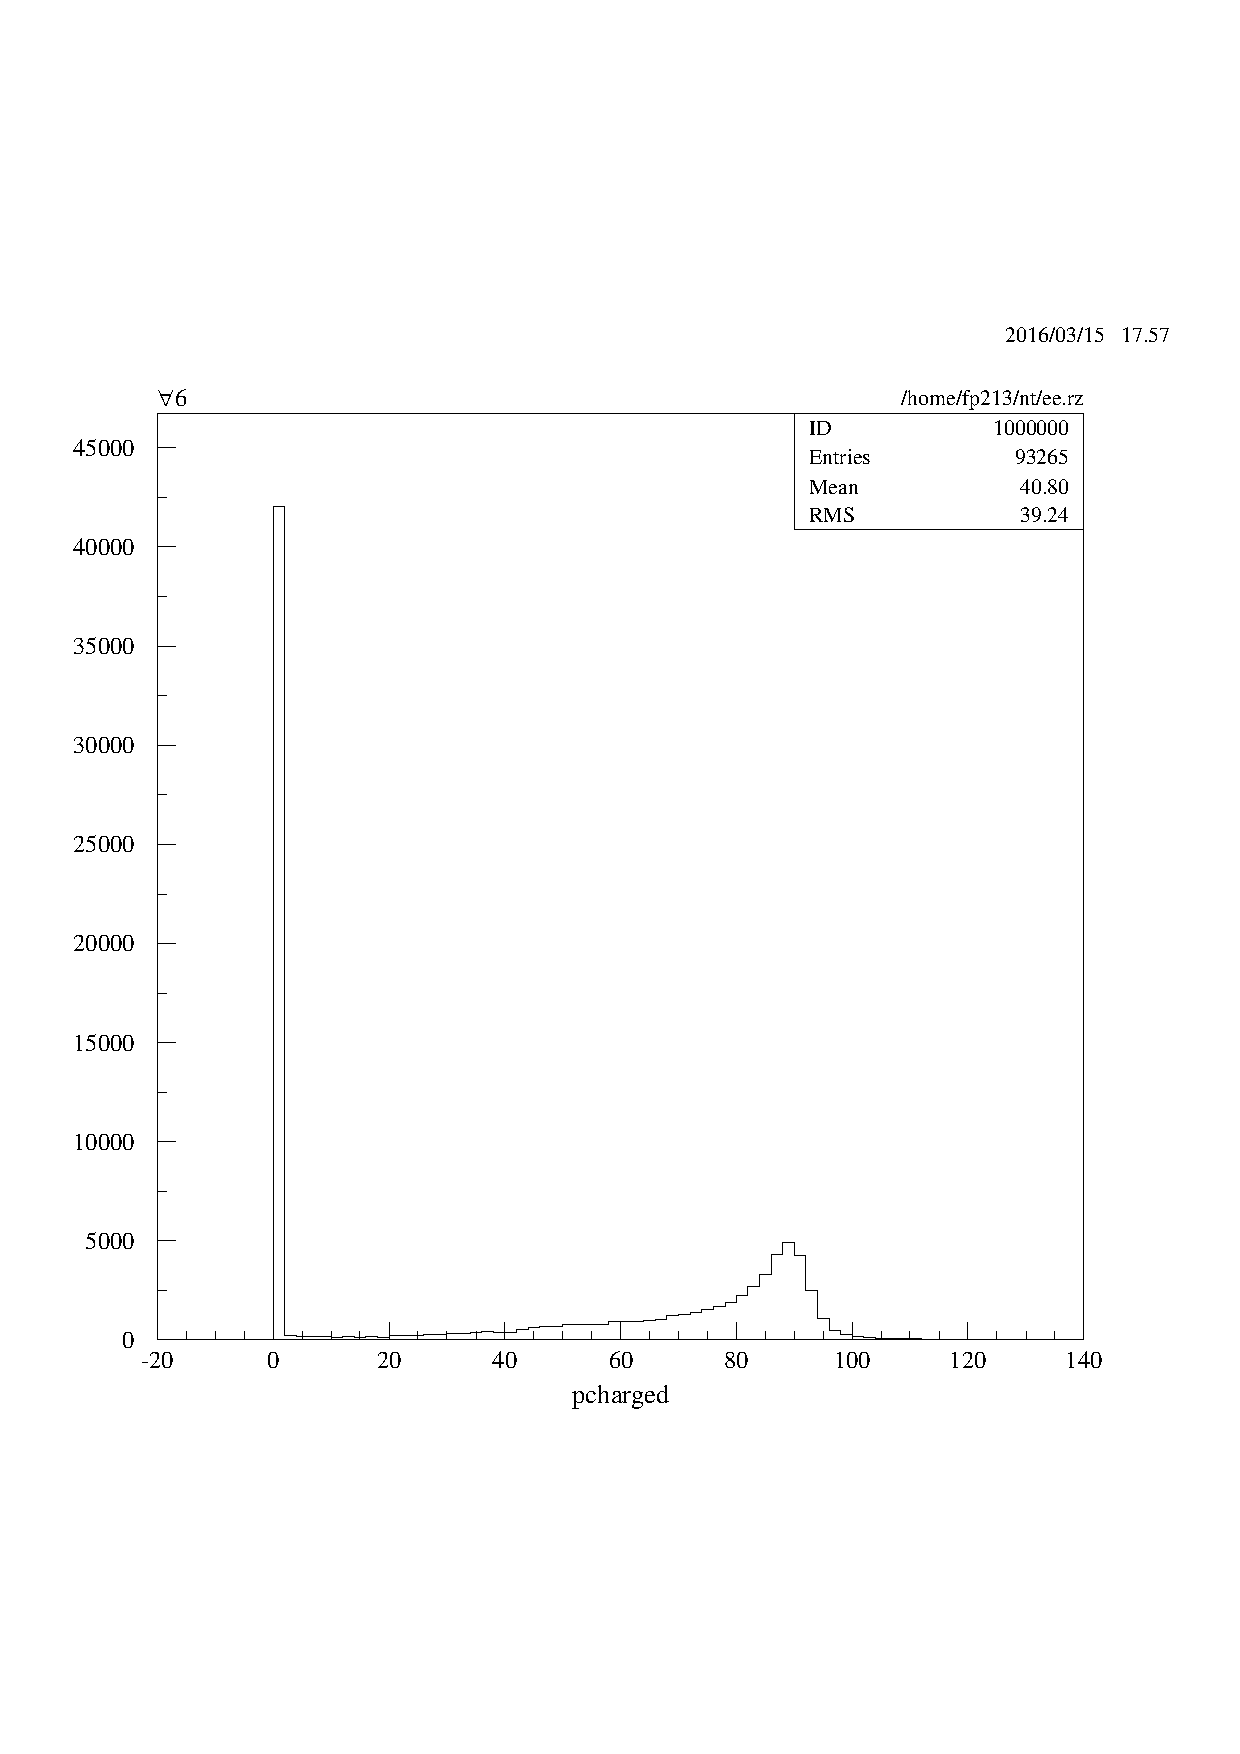
\includegraphics[width=\linewidth]{electrons-pcharged}
        \caption{%
            Electrons
        }
        \label{fig:paw-pcharged/electrons}
    \end{subfigure}
    \hfill
    \begin{subfigure}[c]{0.48\linewidth}
        \centering
        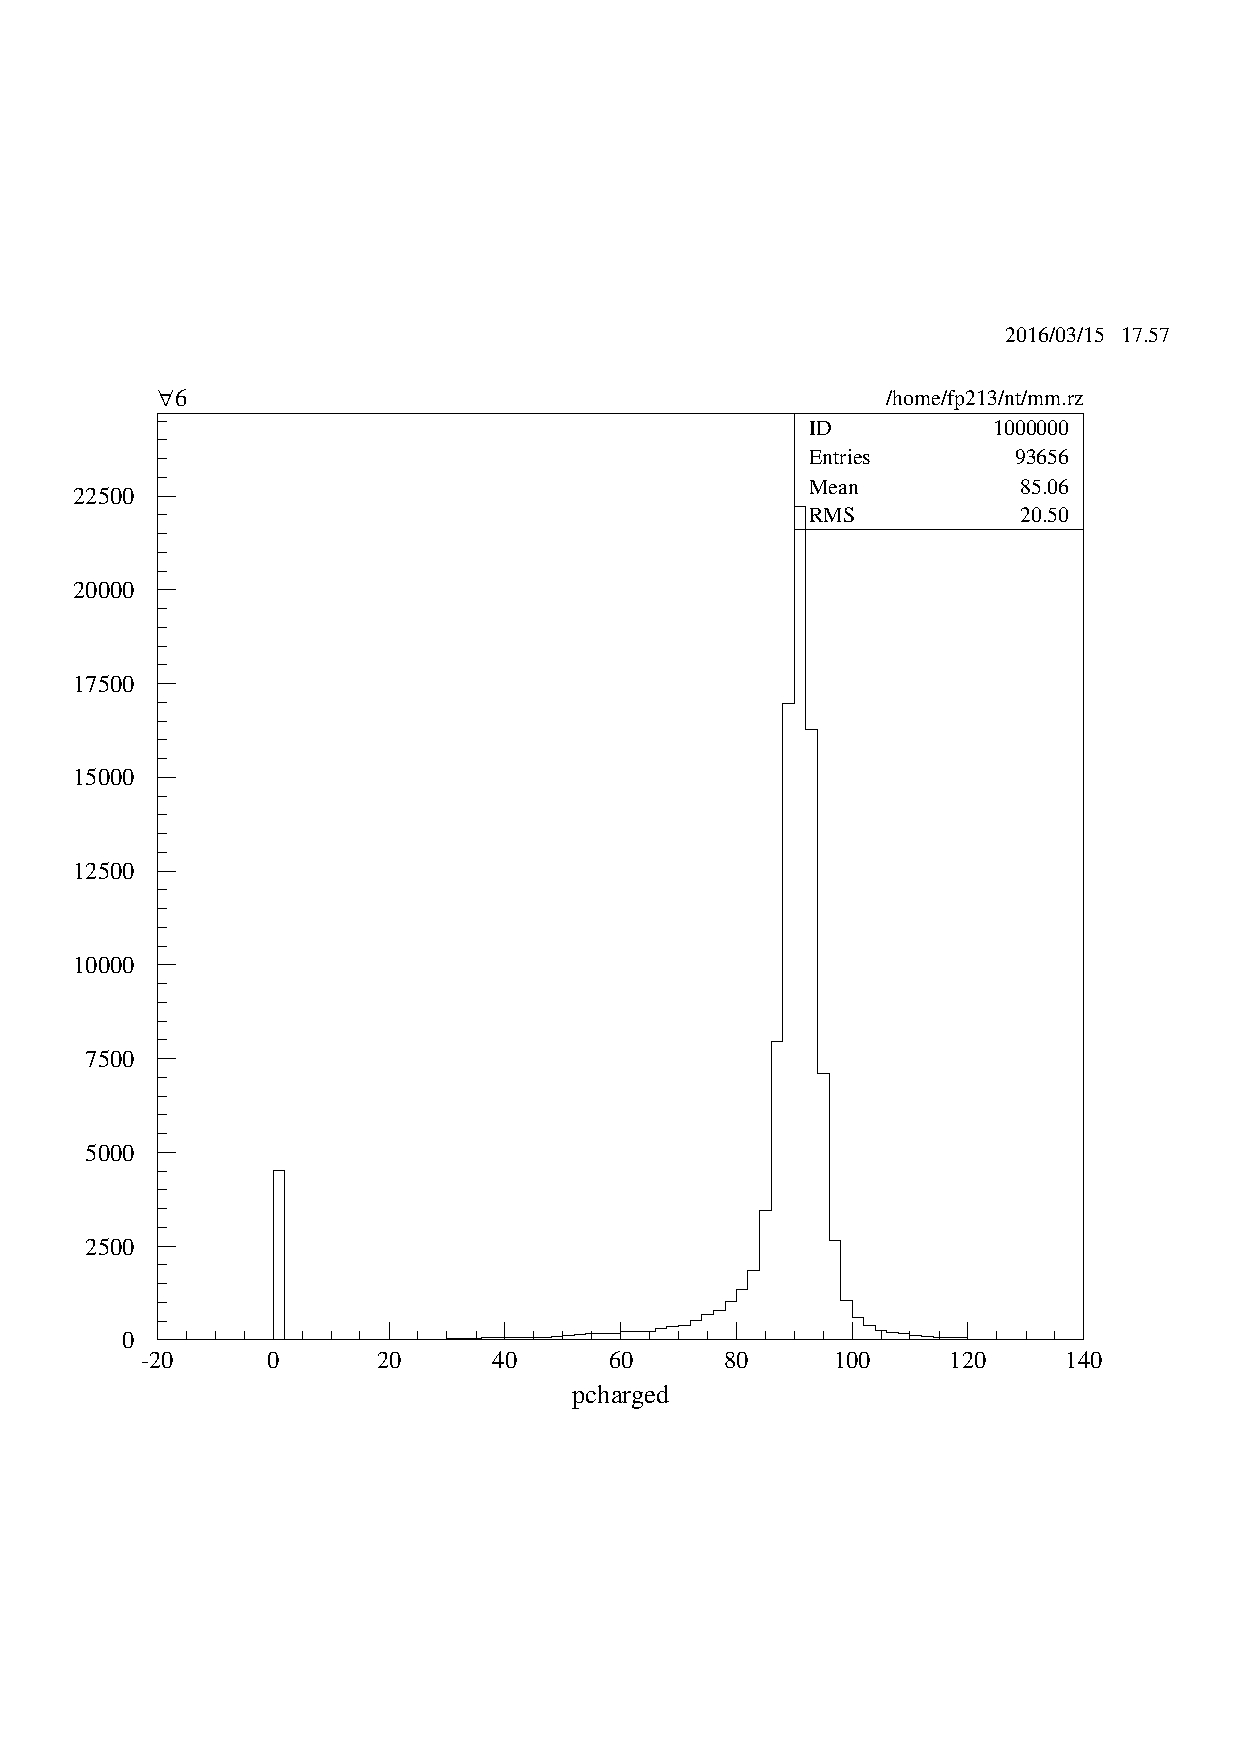
\includegraphics[width=\linewidth]{muons-pcharged}
        \caption{%
            Muons
        }
        \label{fig:paw-pcharged/muons}
    \end{subfigure}

    \vspace{2ex}

    \begin{subfigure}[c]{0.48\linewidth}
        \centering
        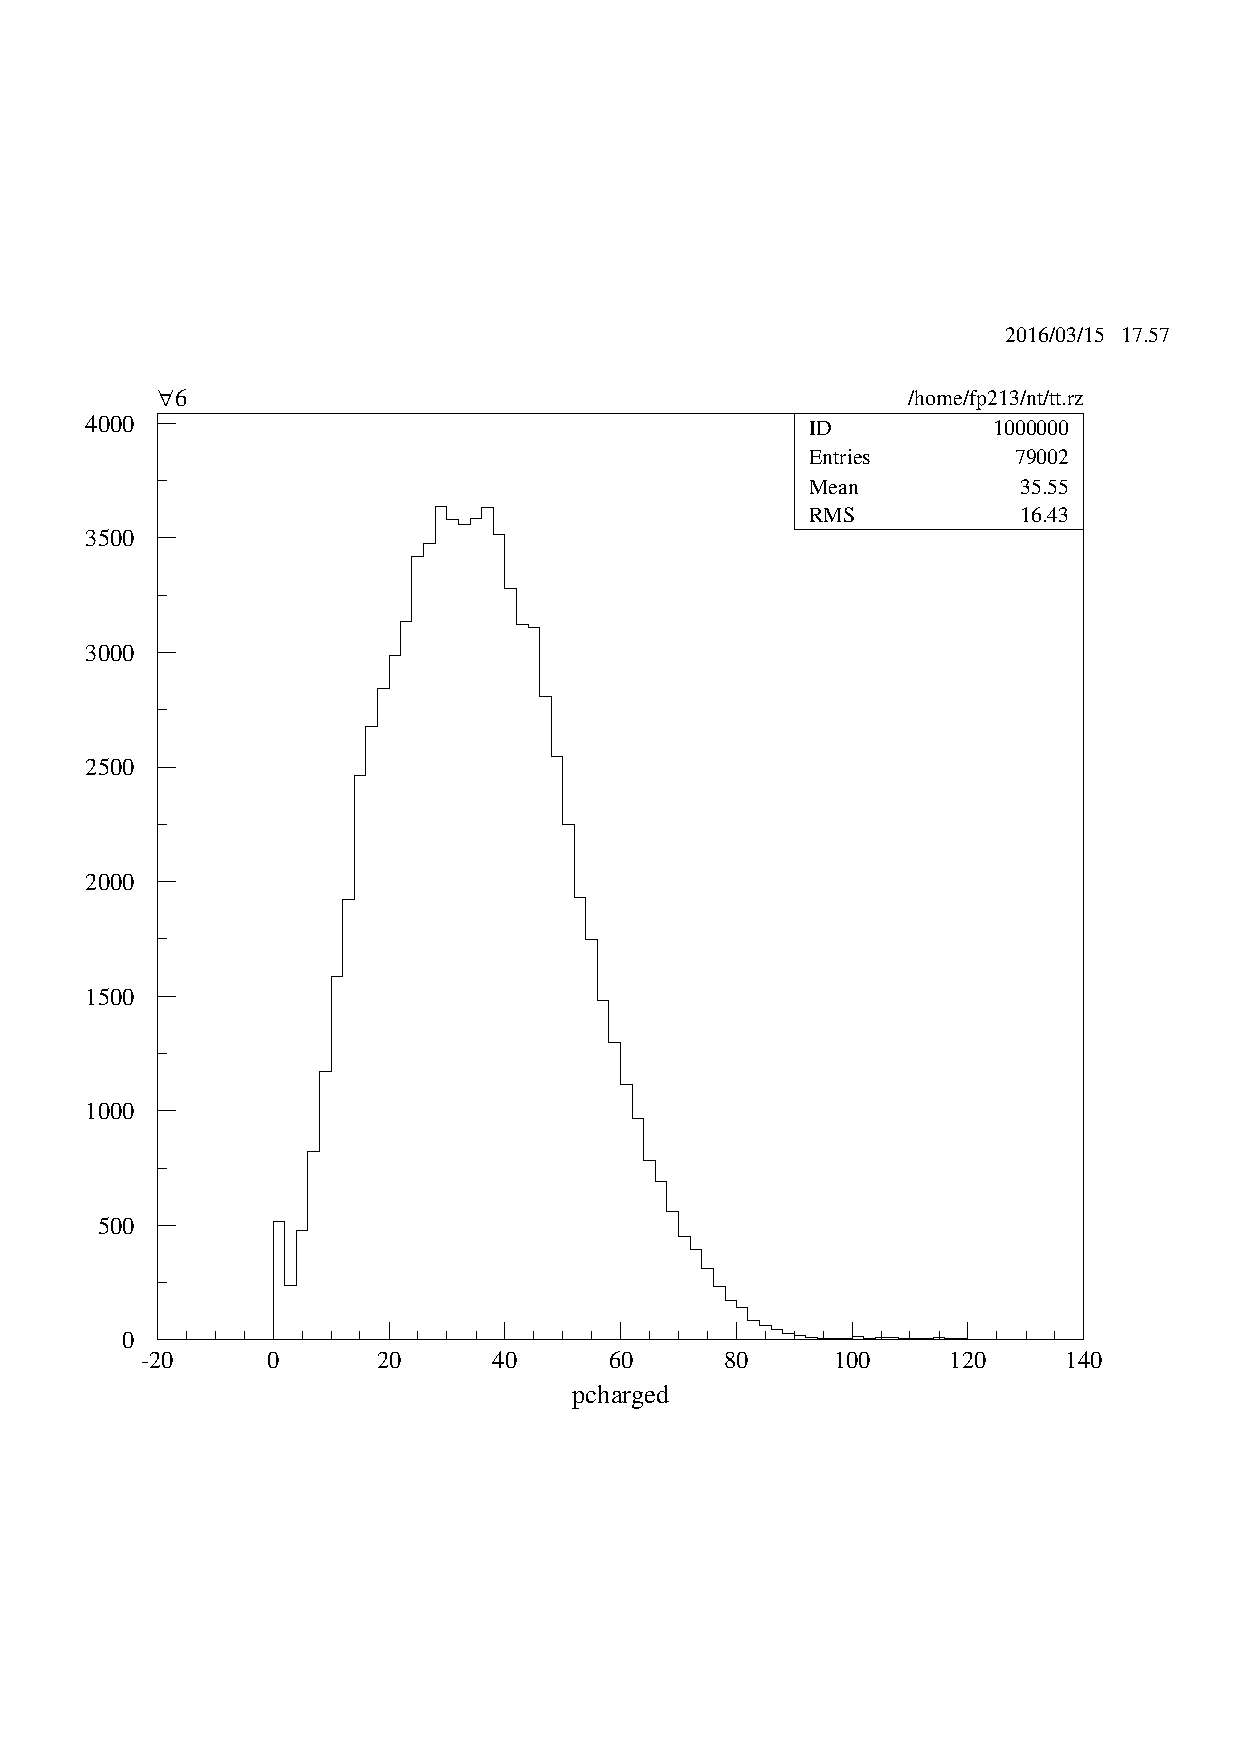
\includegraphics[width=\linewidth]{taus-pcharged}
        \caption{%
            Tauons
        }
        \label{fig:paw-pcharged/tauons}
    \end{subfigure}
    \hfill
    \begin{subfigure}[c]{0.48\linewidth}
        \centering
        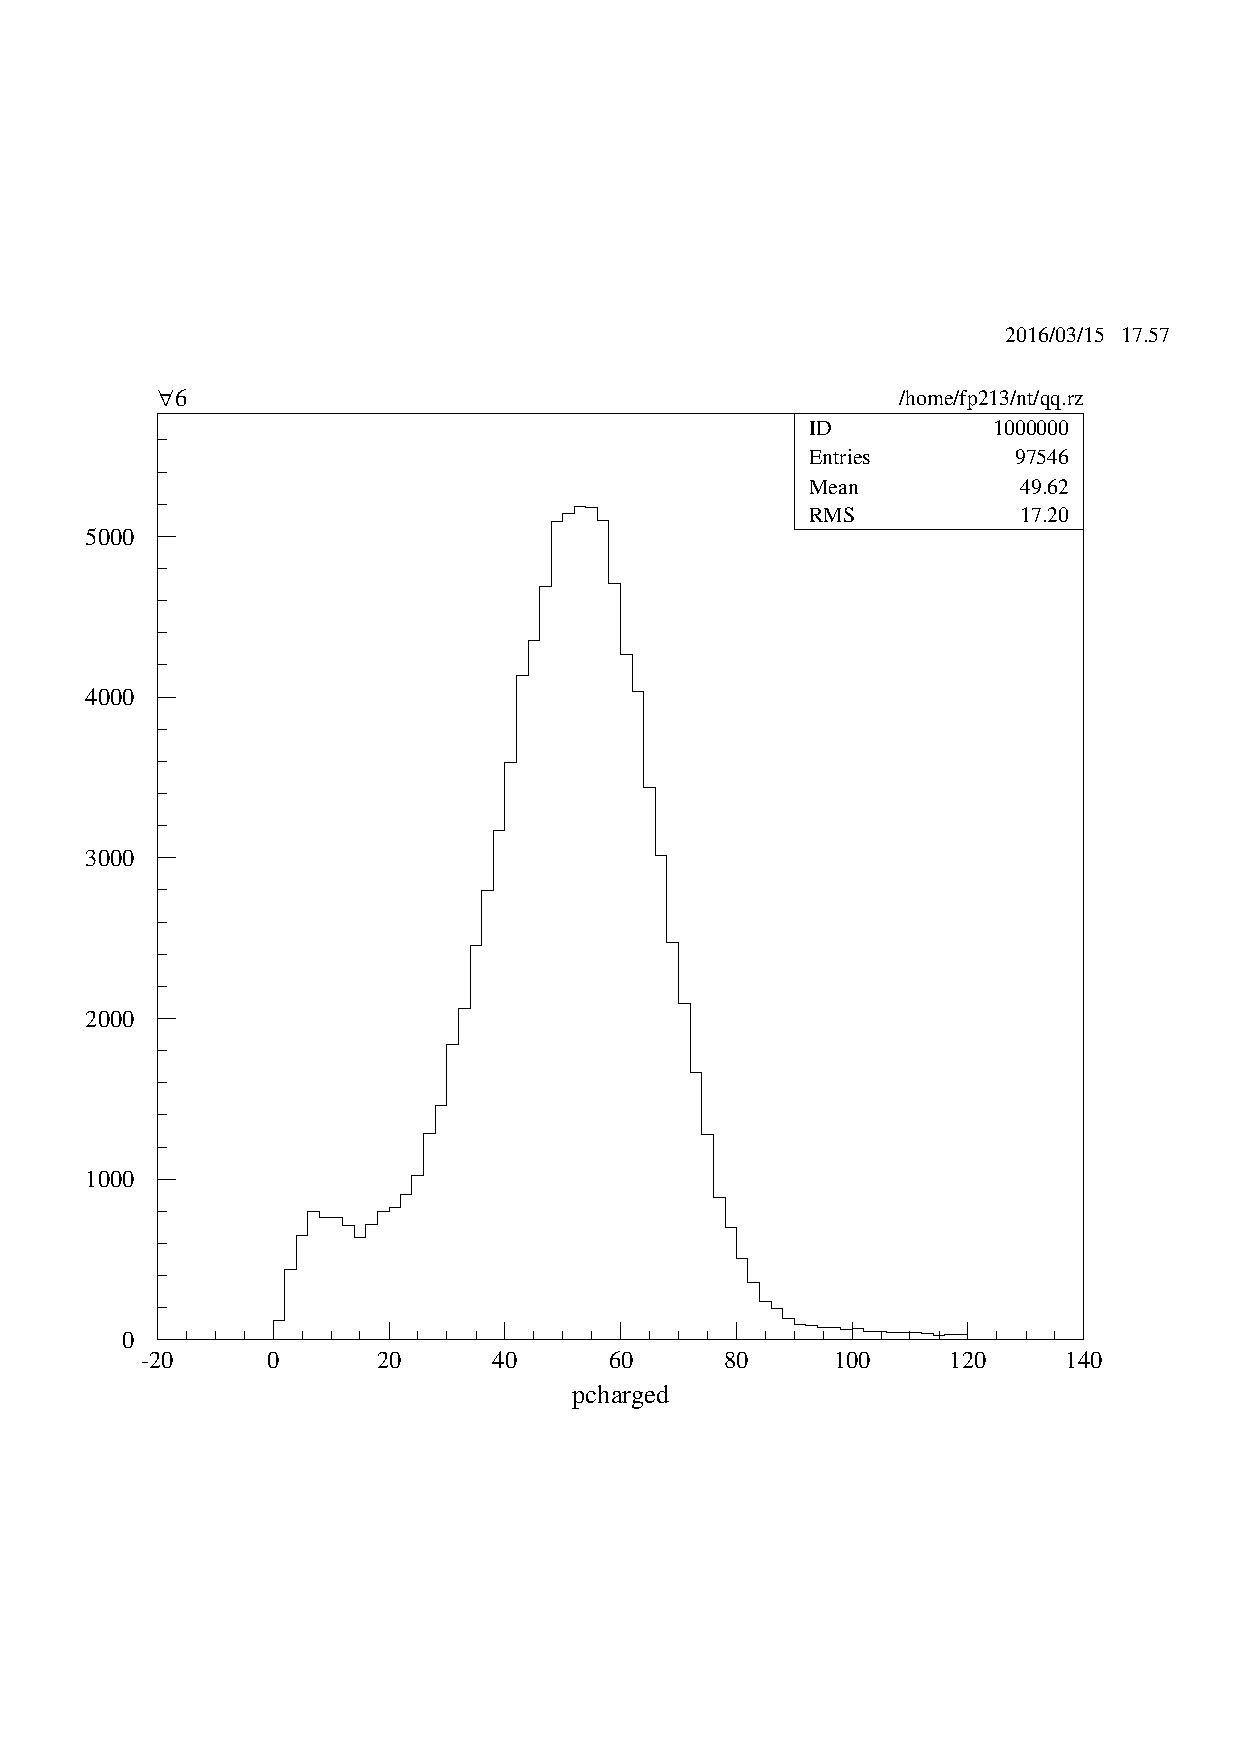
\includegraphics[width=\linewidth]{hadrons-pcharged}
        \caption{%
            Hadrons
        }
        \label{fig:paw-pcharged/hadrons}
    \end{subfigure}
    \caption{%
        Energy in charged tracks, \pcharged, for the four decay types.
        Histograms generated with \textsc{paw} from Monte Carlo datasets.
    }
    \label{fig:paw-pcharged}
\end{figure}


    \begin{figure}
    \centering
    \begin{subfigure}[c]{0.48\linewidth}
        \centering
        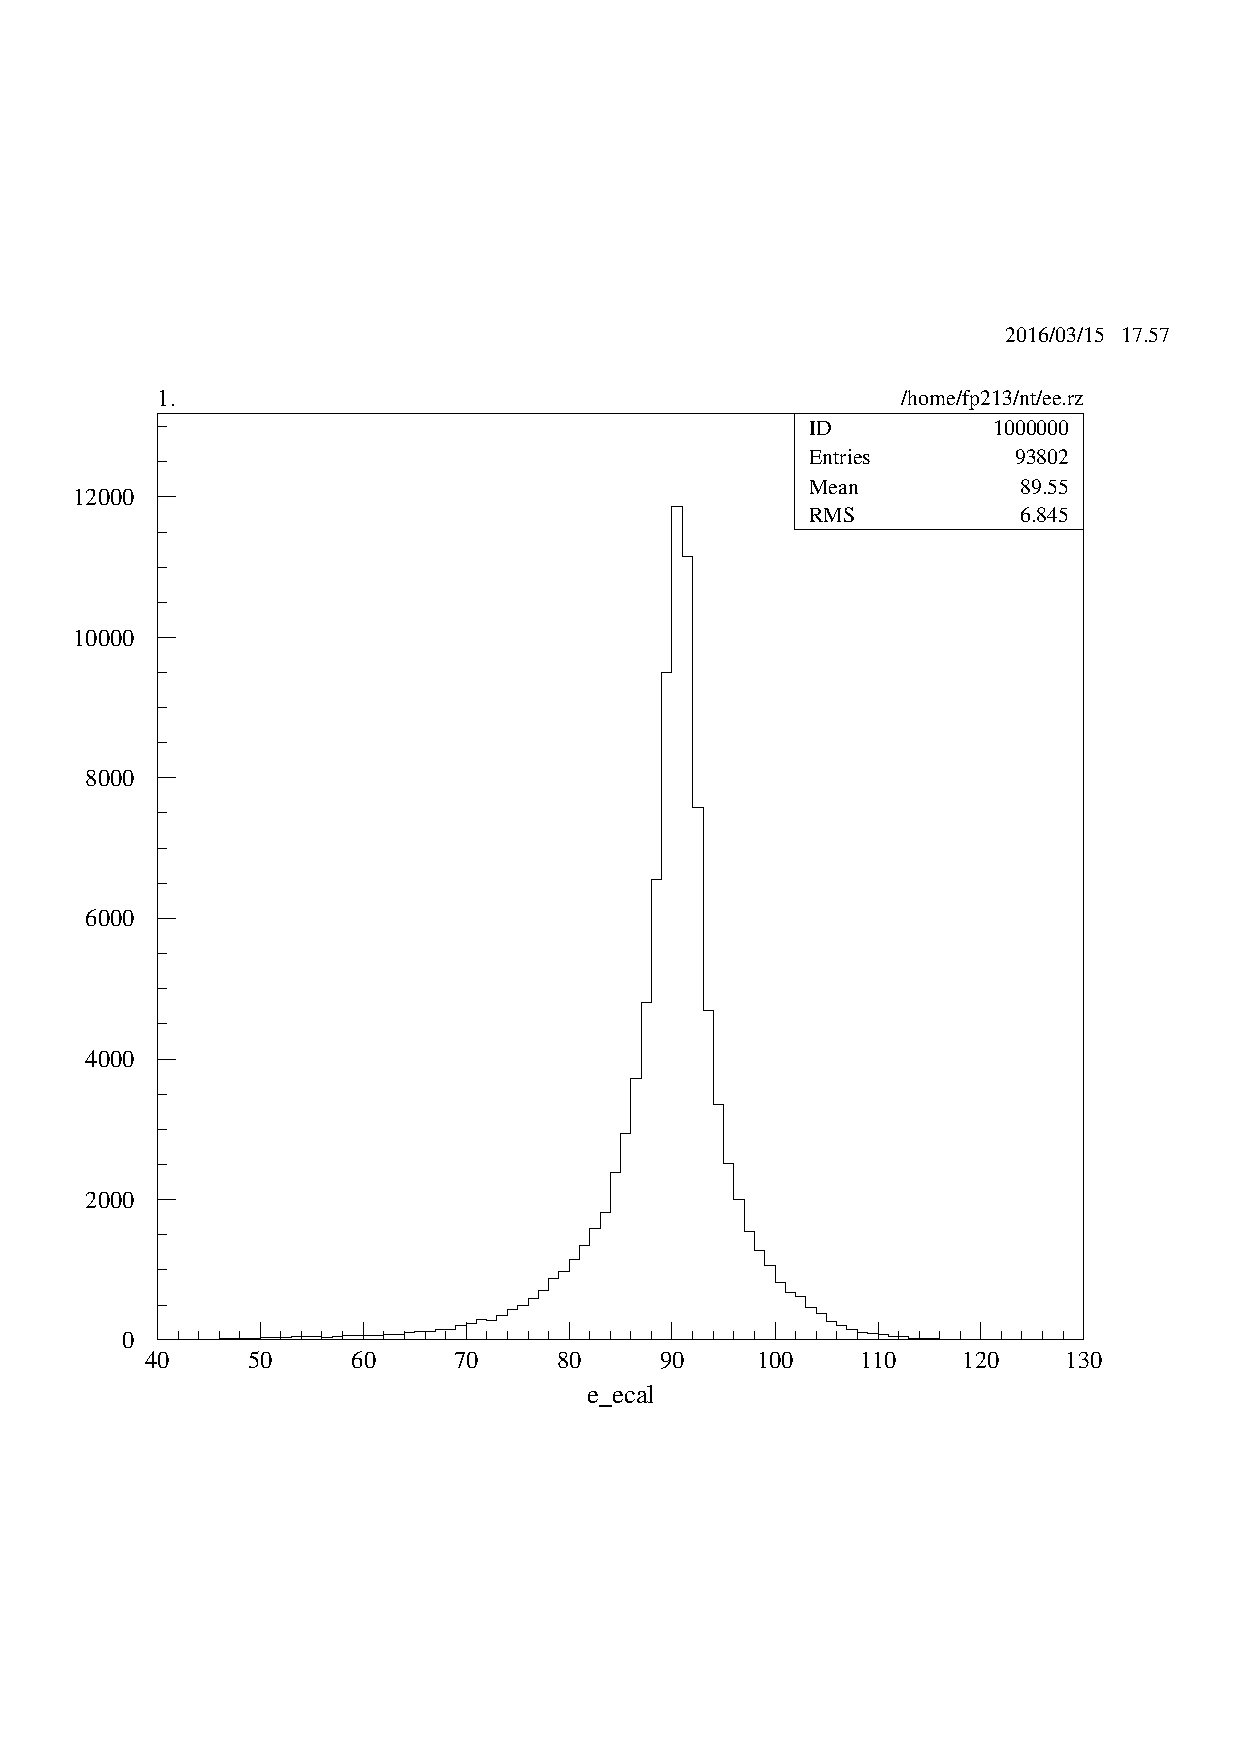
\includegraphics[width=\linewidth]{electrons-e_ecal}
        \caption{%
            Electrons
        }
        \label{fig:paw-e_ecal/electrons}
    \end{subfigure}
    \hfill
    \begin{subfigure}[c]{0.48\linewidth}
        \centering
        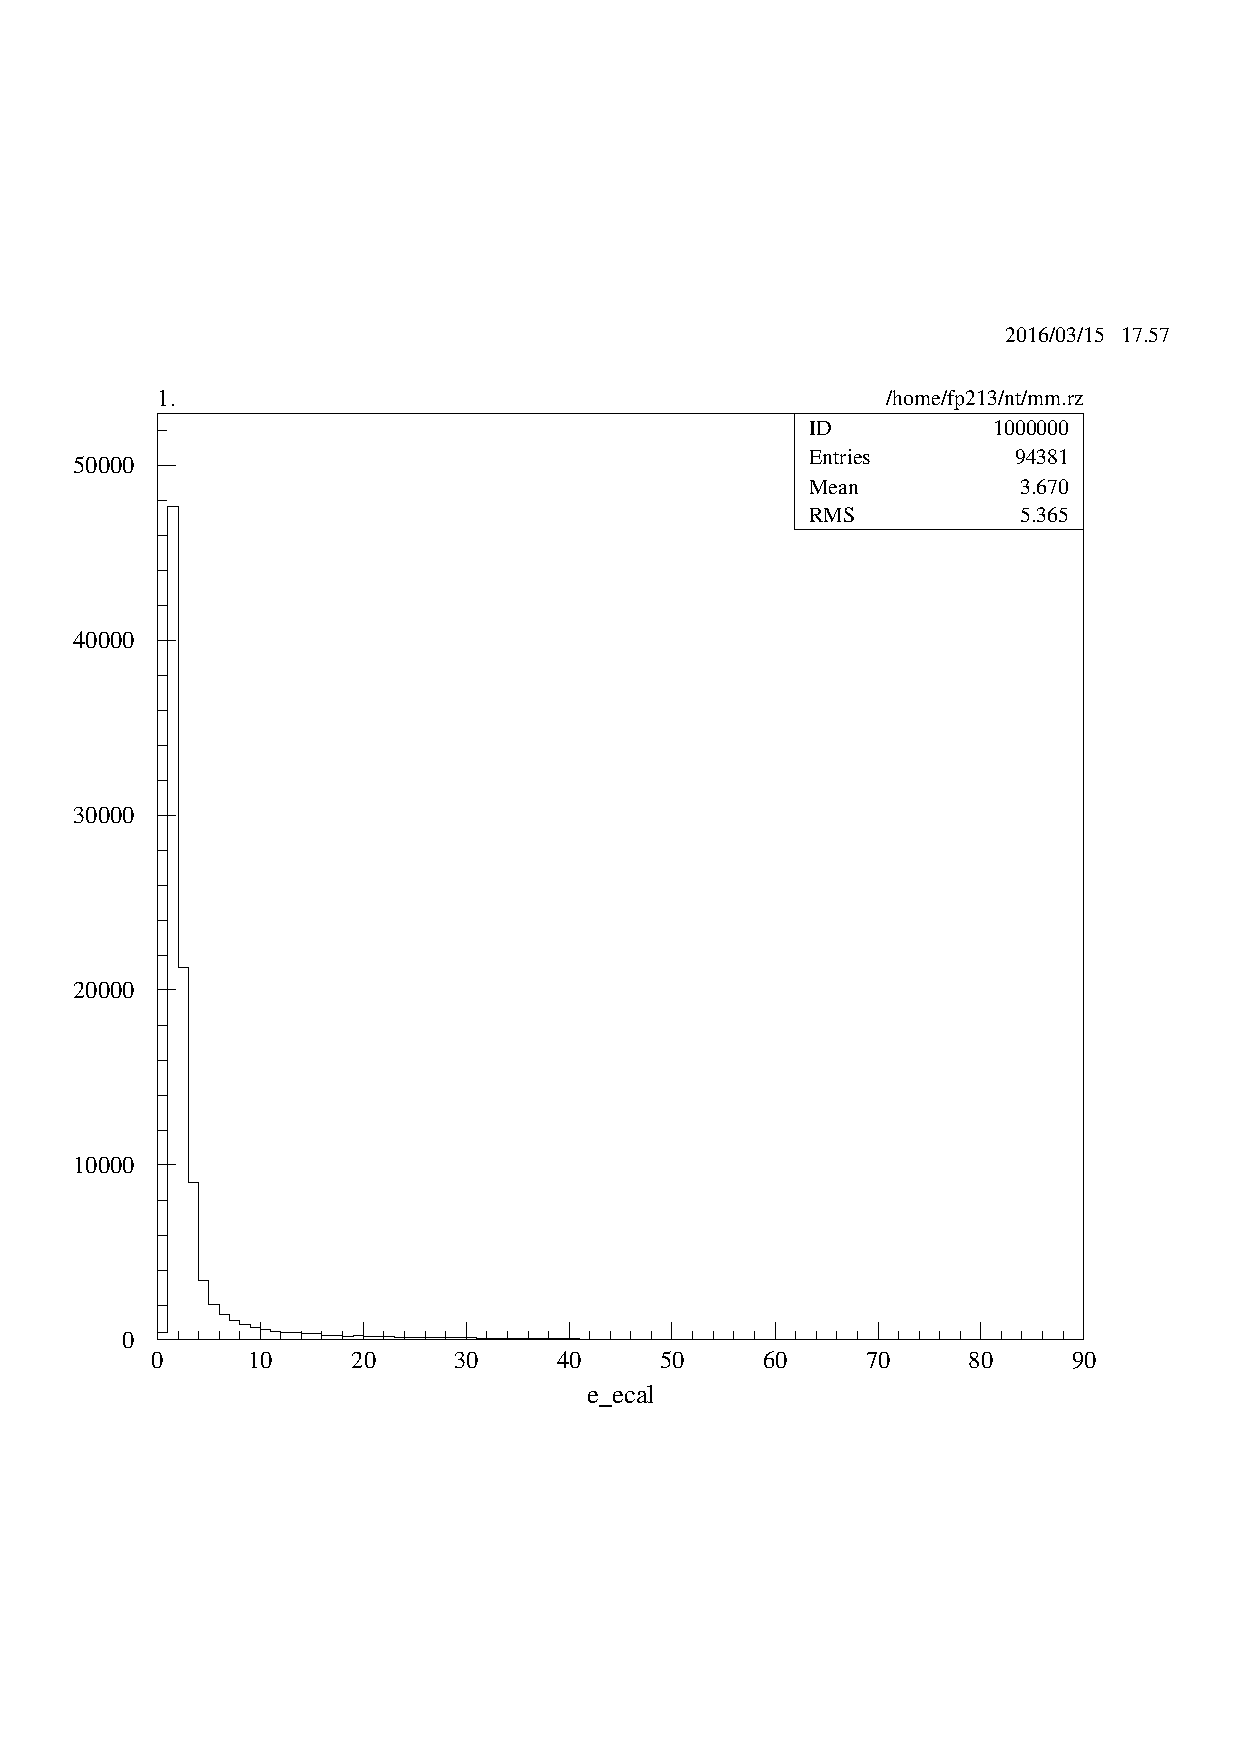
\includegraphics[width=\linewidth]{muons-e_ecal}
        \caption{%
            Muons
        }
        \label{fig:paw-e_ecal/muons}
    \end{subfigure}

    \vspace{2ex}

    \begin{subfigure}[c]{0.48\linewidth}
        \centering
        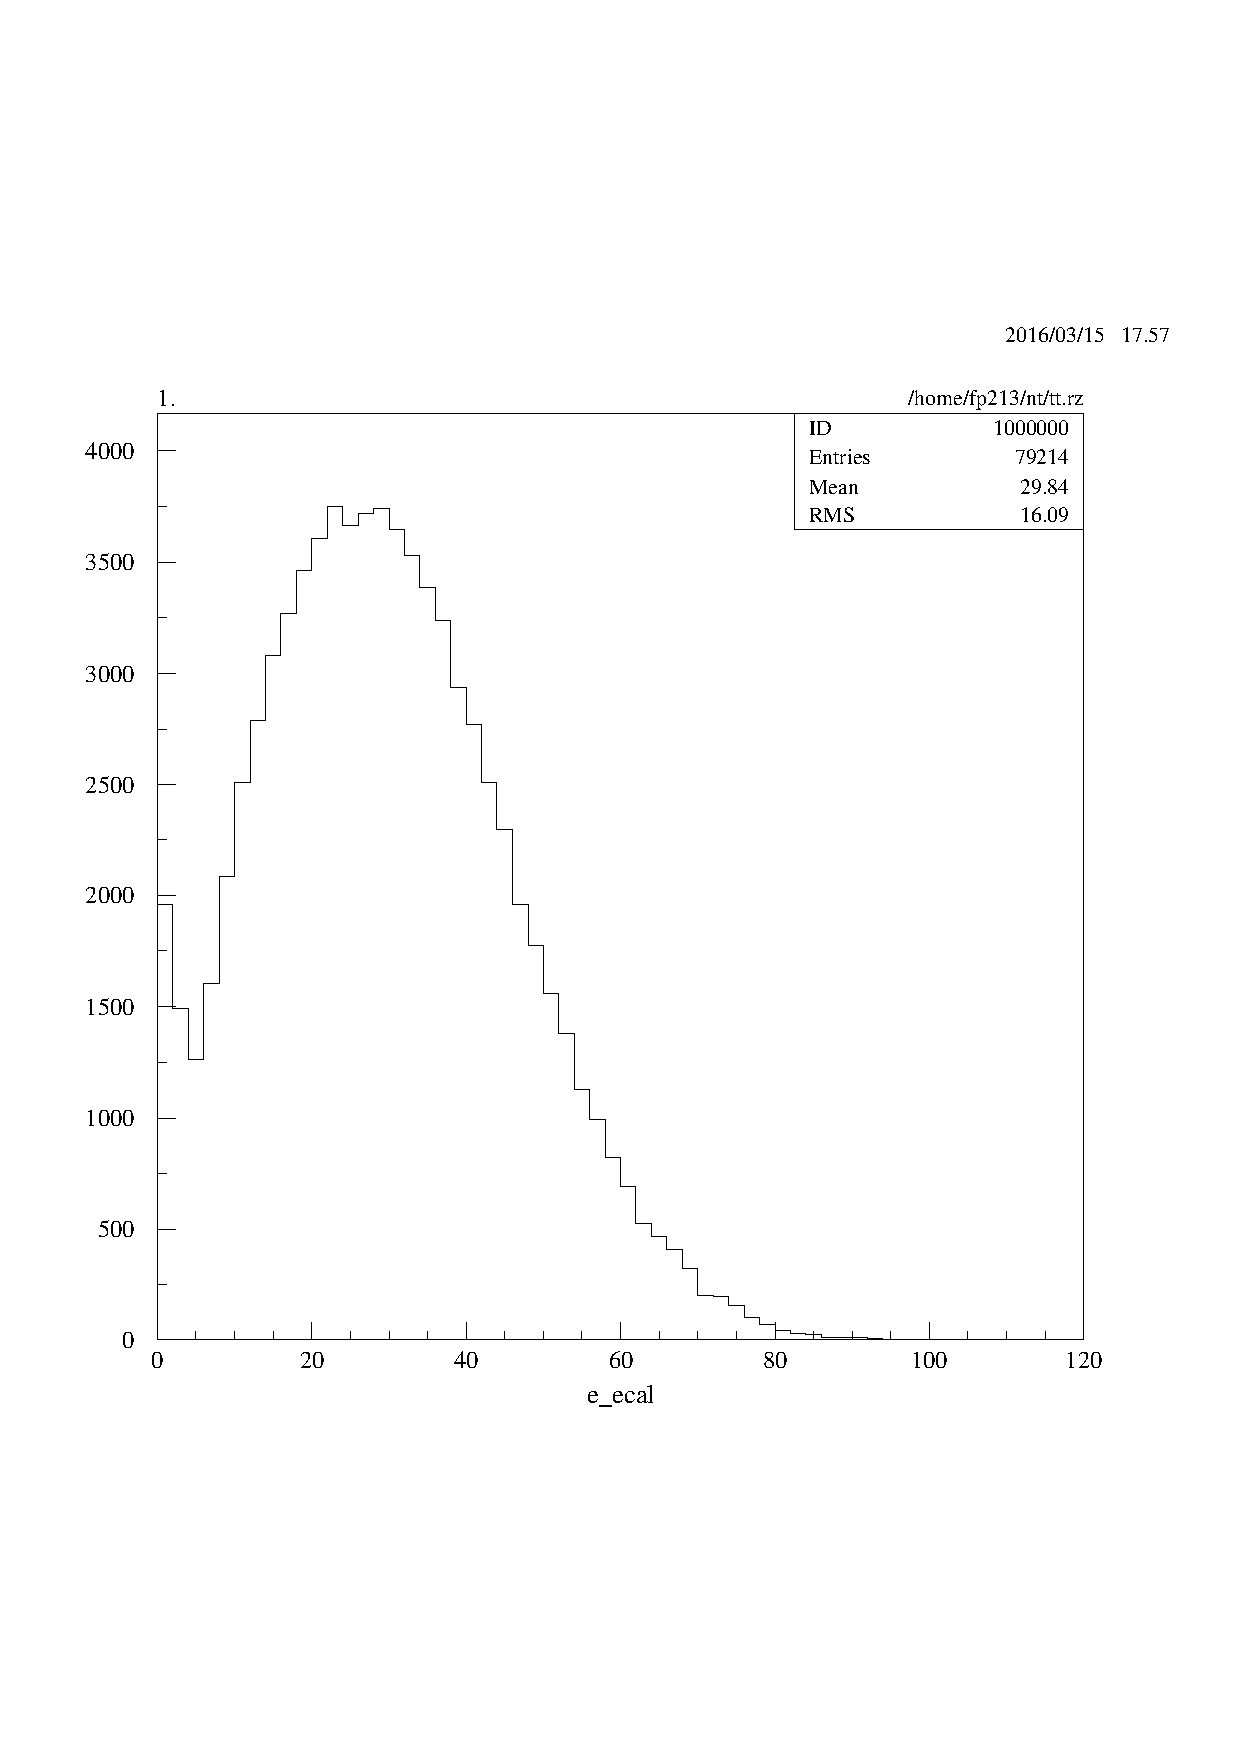
\includegraphics[width=\linewidth]{taus-e_ecal}
        \caption{%
            Taus
        }
        \label{fig:paw-e_ecal/taus}
    \end{subfigure}
    \hfill
    \begin{subfigure}[c]{0.48\linewidth}
        \centering
        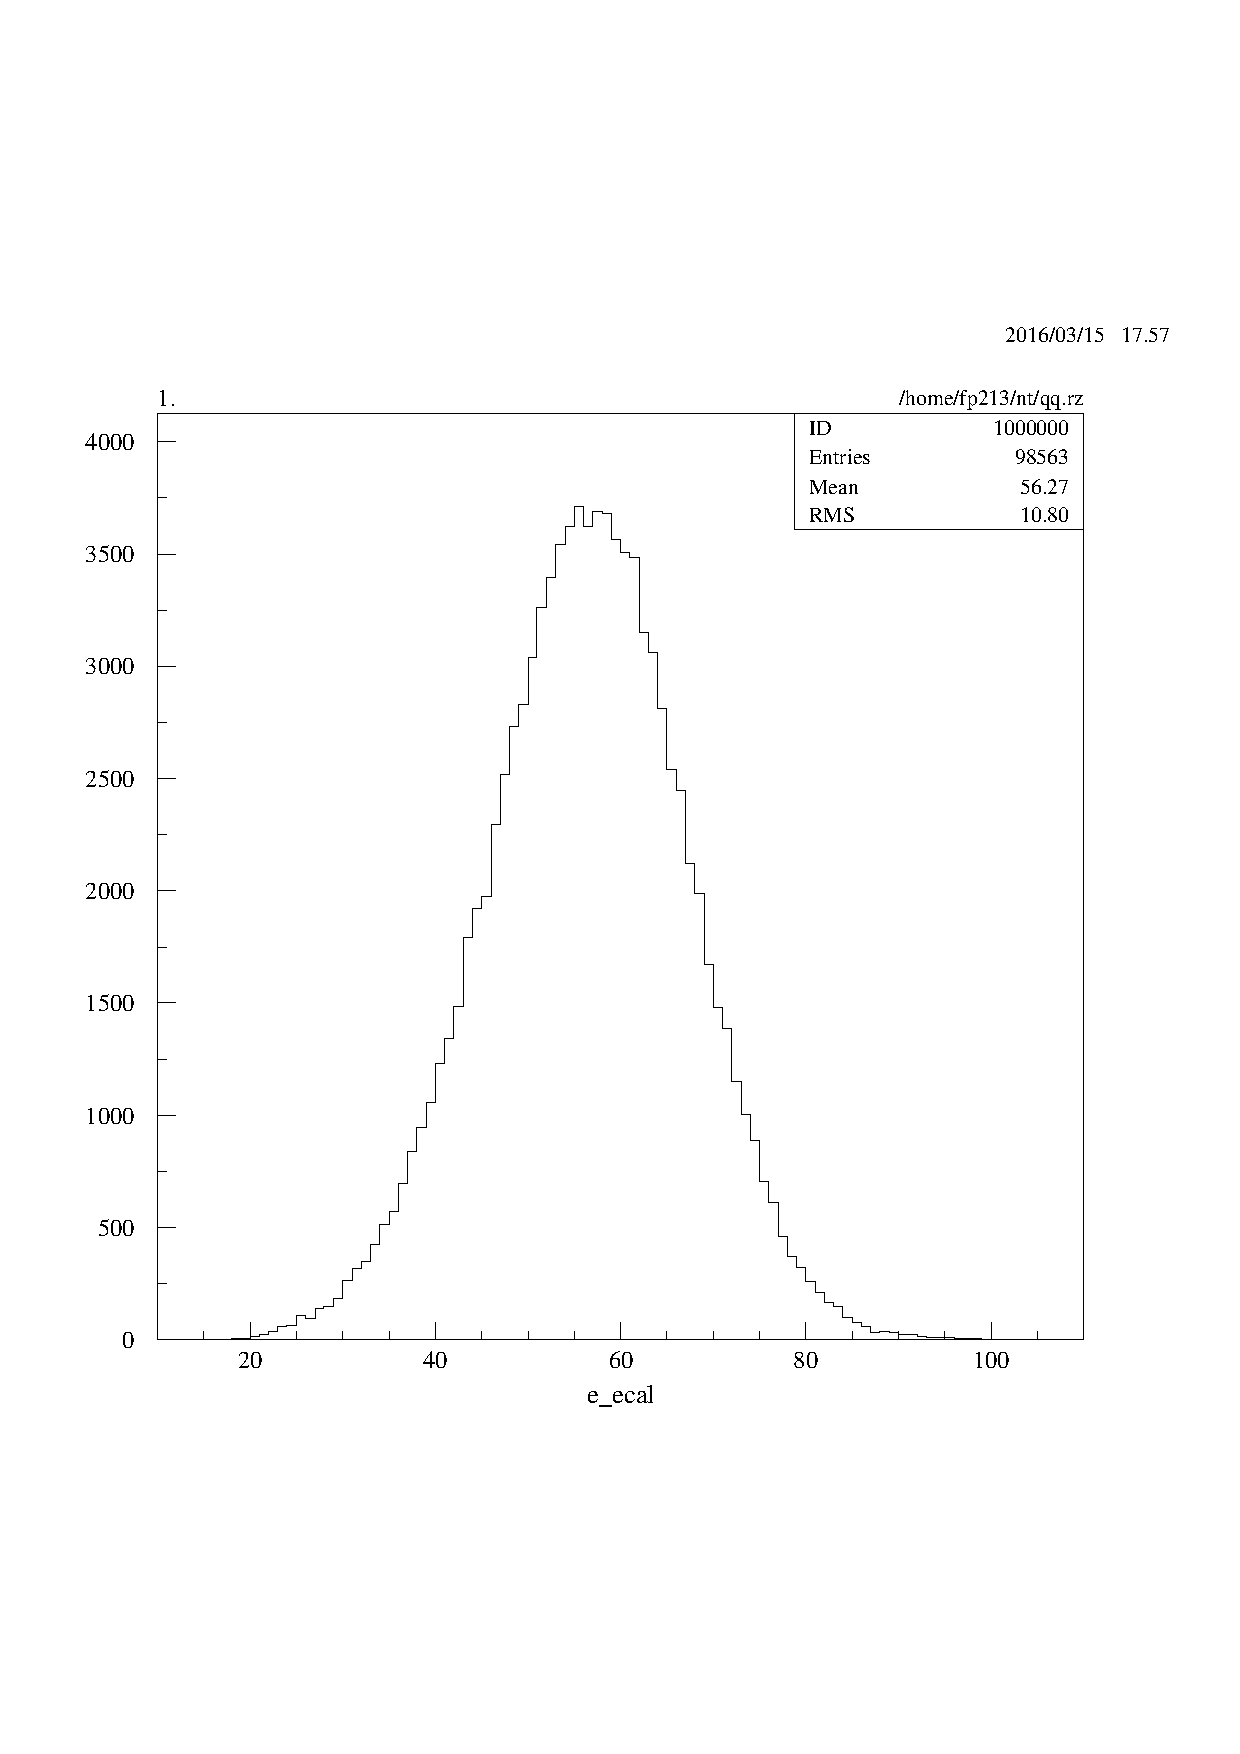
\includegraphics[width=\linewidth]{hadrons-e_ecal}
        \caption{%
            Hadrons
        }
        \label{fig:paw-e_ecal/hadrons}
    \end{subfigure}
    \caption{%
        Energy deposited into the \ecal\ for the four decay types.
        Histograms generated with \textsc{paw} from Monte Carlo datasets.
    }
    \label{fig:paw-e_ecal}
\end{figure}


    \begin{figure}
    \centering
    \begin{subfigure}[c]{0.48\linewidth}
        \centering
        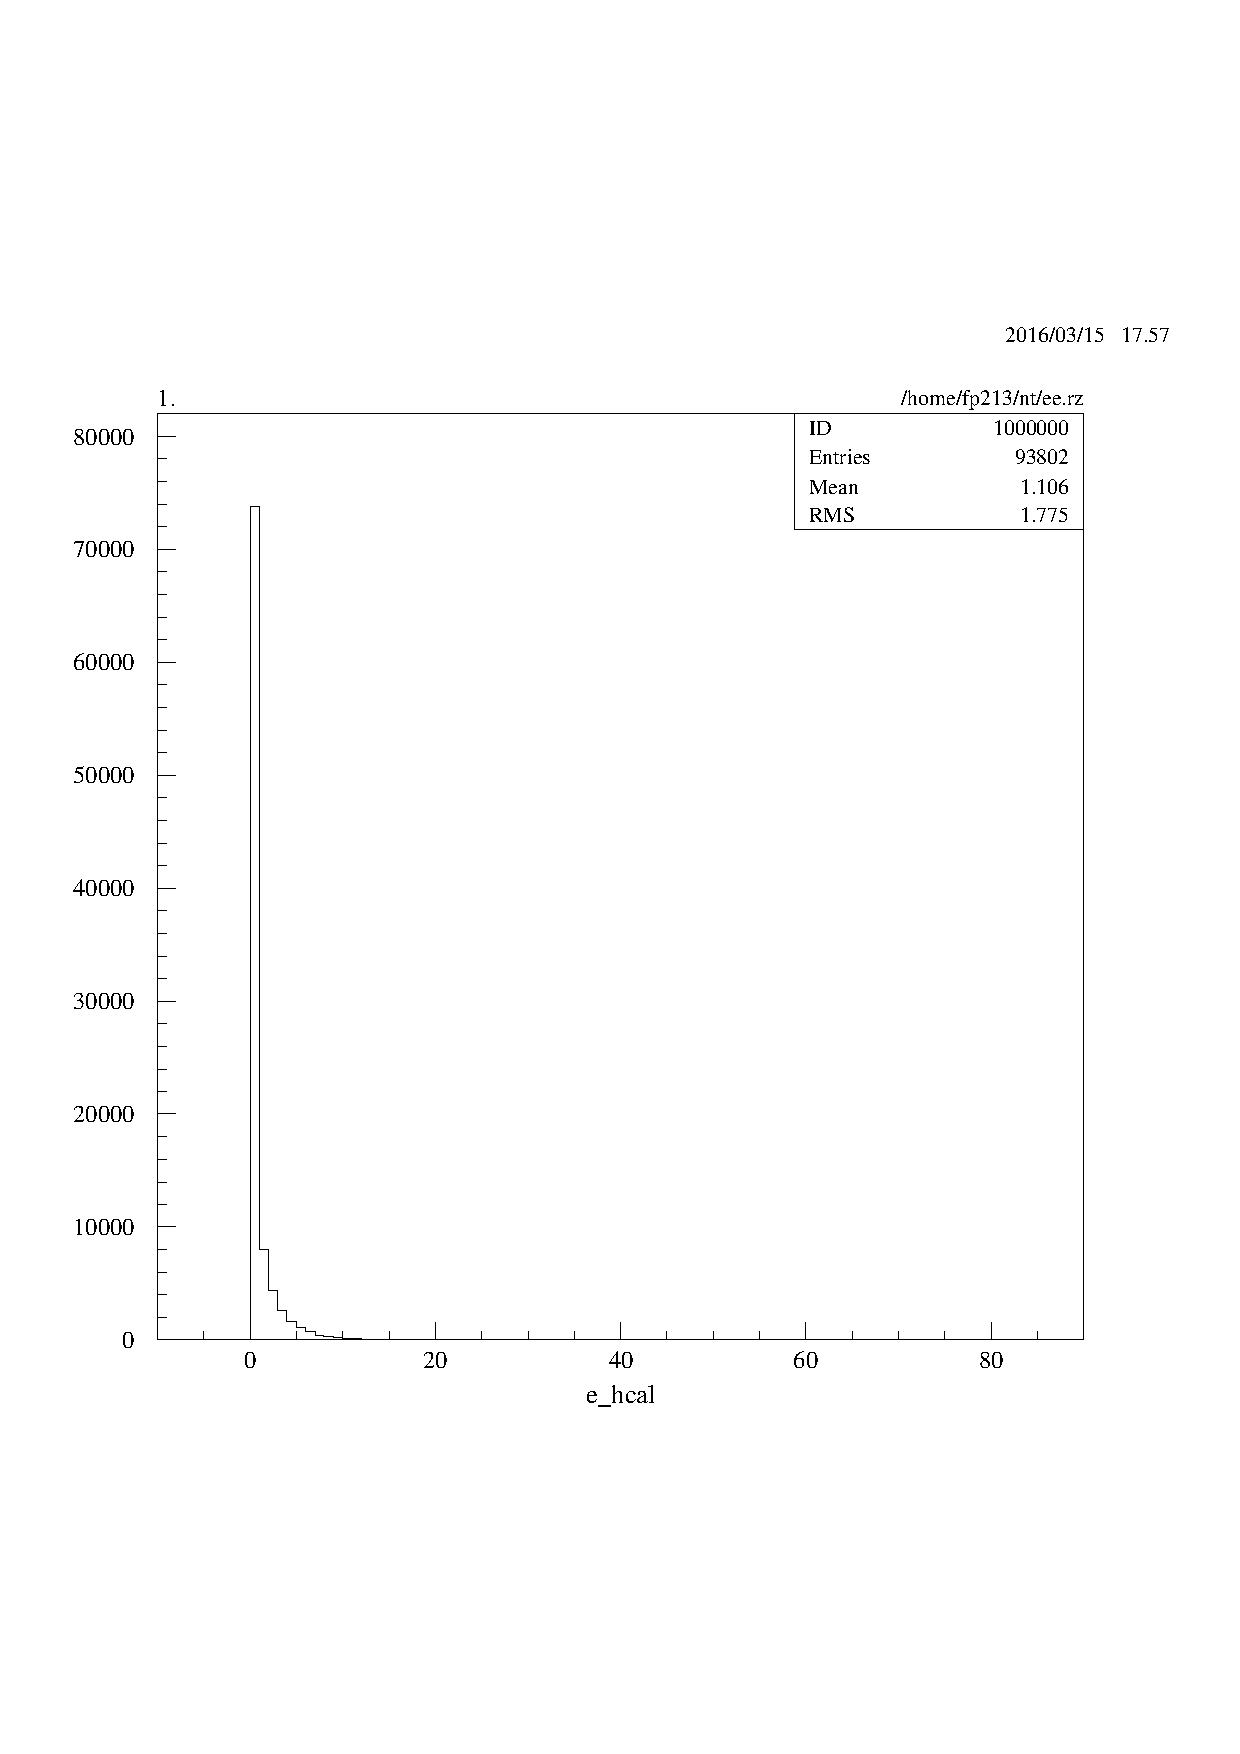
\includegraphics[width=\linewidth]{electrons-e_hcal}
        \caption{%
            Electrons
        }
        \label{fig:paw-e_hcal/electrons}
    \end{subfigure}
    \hfill
    \begin{subfigure}[c]{0.48\linewidth}
        \centering
        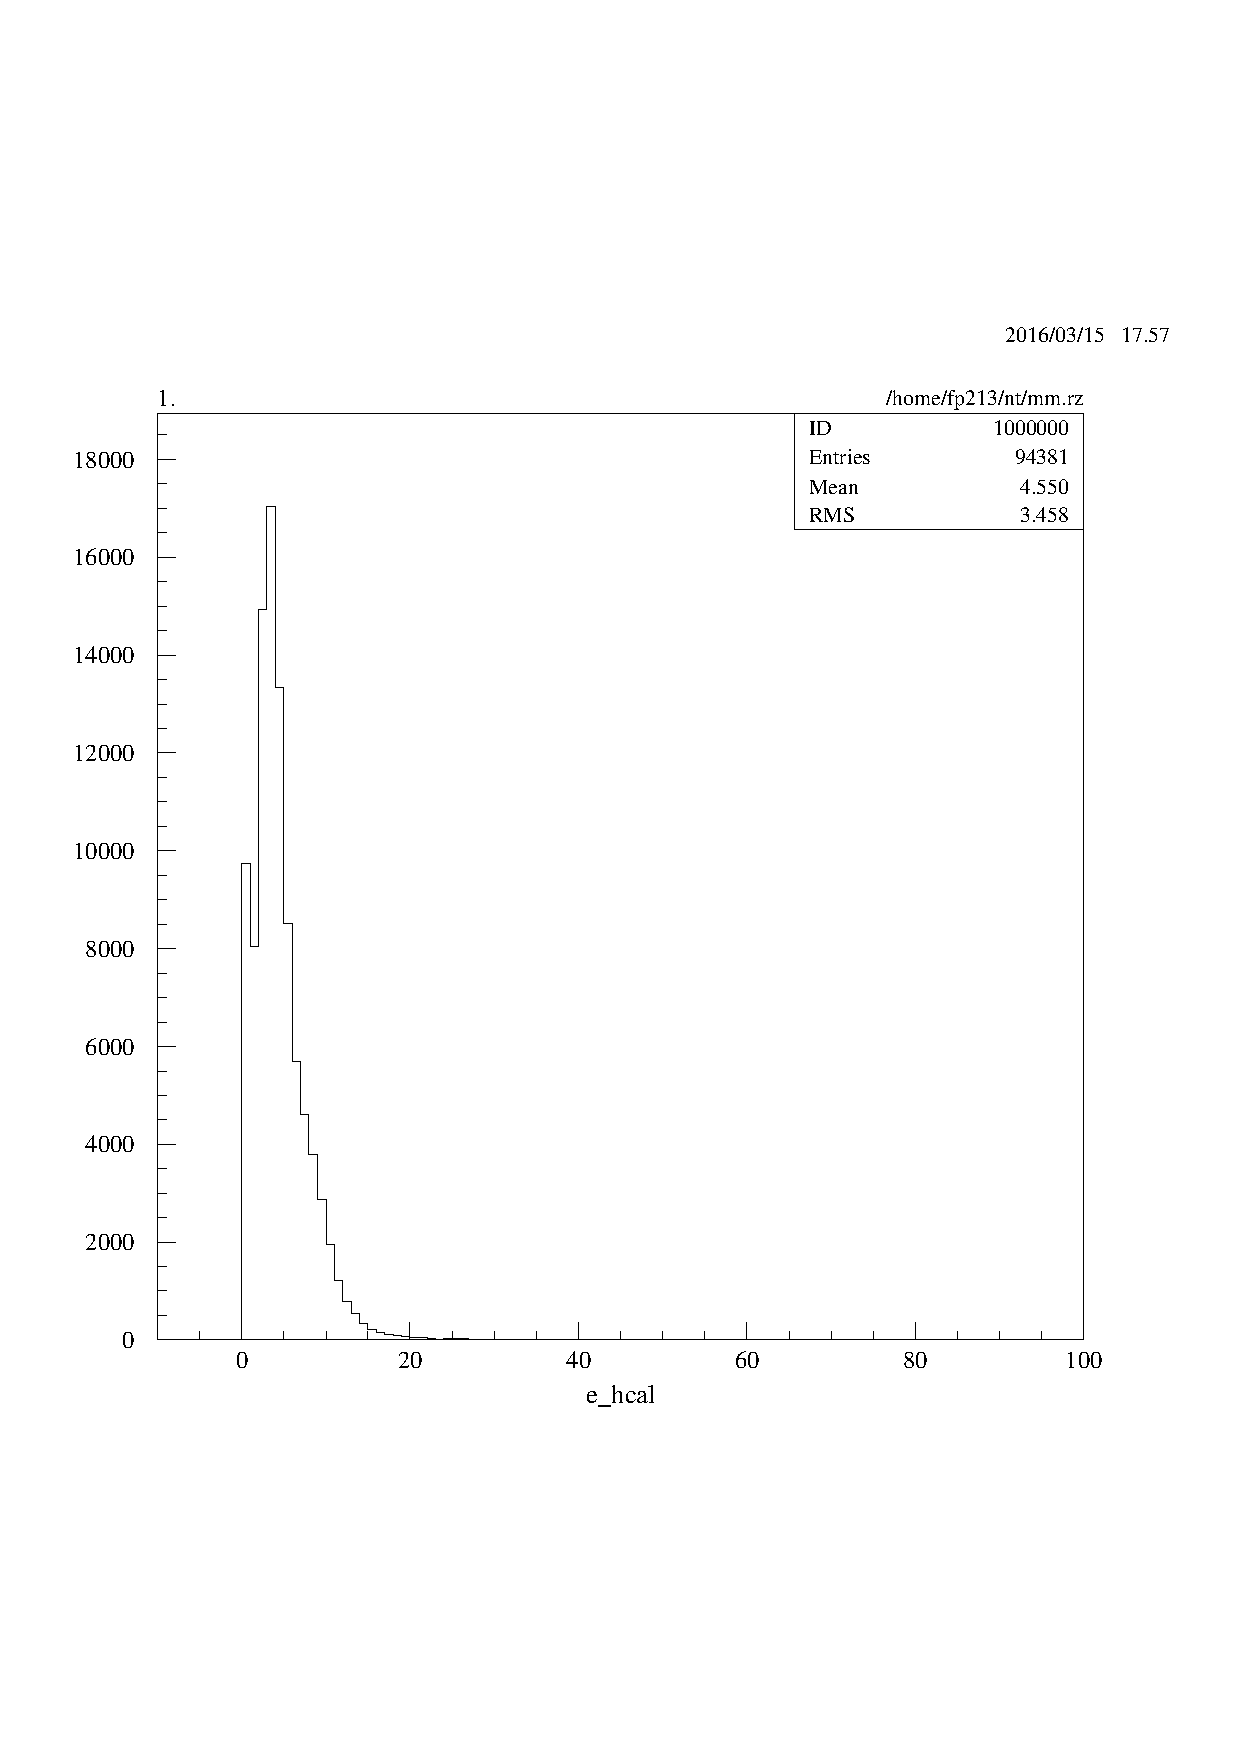
\includegraphics[width=\linewidth]{muons-e_hcal}
        \caption{%
            Muons
        }
        \label{fig:paw-e_hcal/muons}
    \end{subfigure}

    \vspace{2ex}

    \begin{subfigure}[c]{0.48\linewidth}
        \centering
        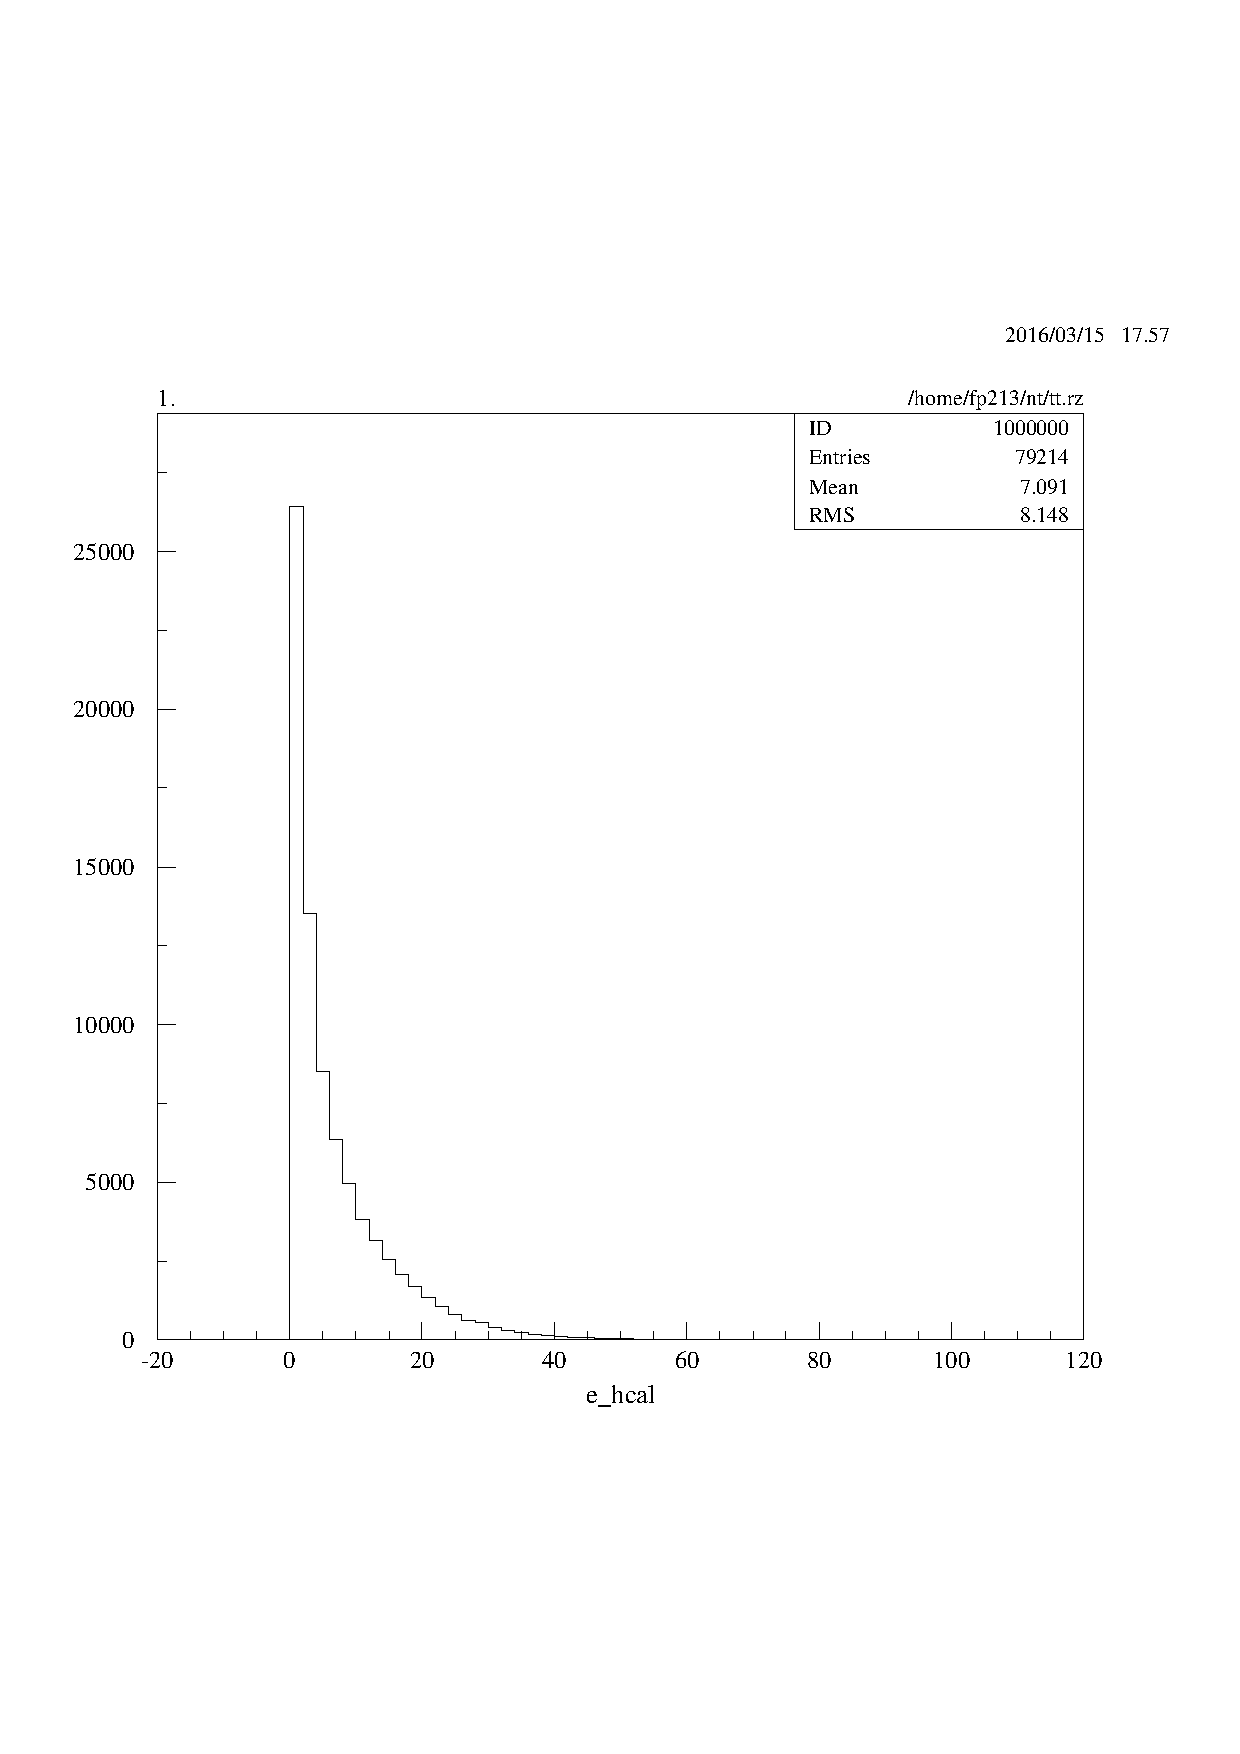
\includegraphics[width=\linewidth]{taus-e_hcal}
        \caption{%
            Taus
        }
        \label{fig:paw-e_hcal/taus}
    \end{subfigure}
    \hfill
    \begin{subfigure}[c]{0.48\linewidth}
        \centering
        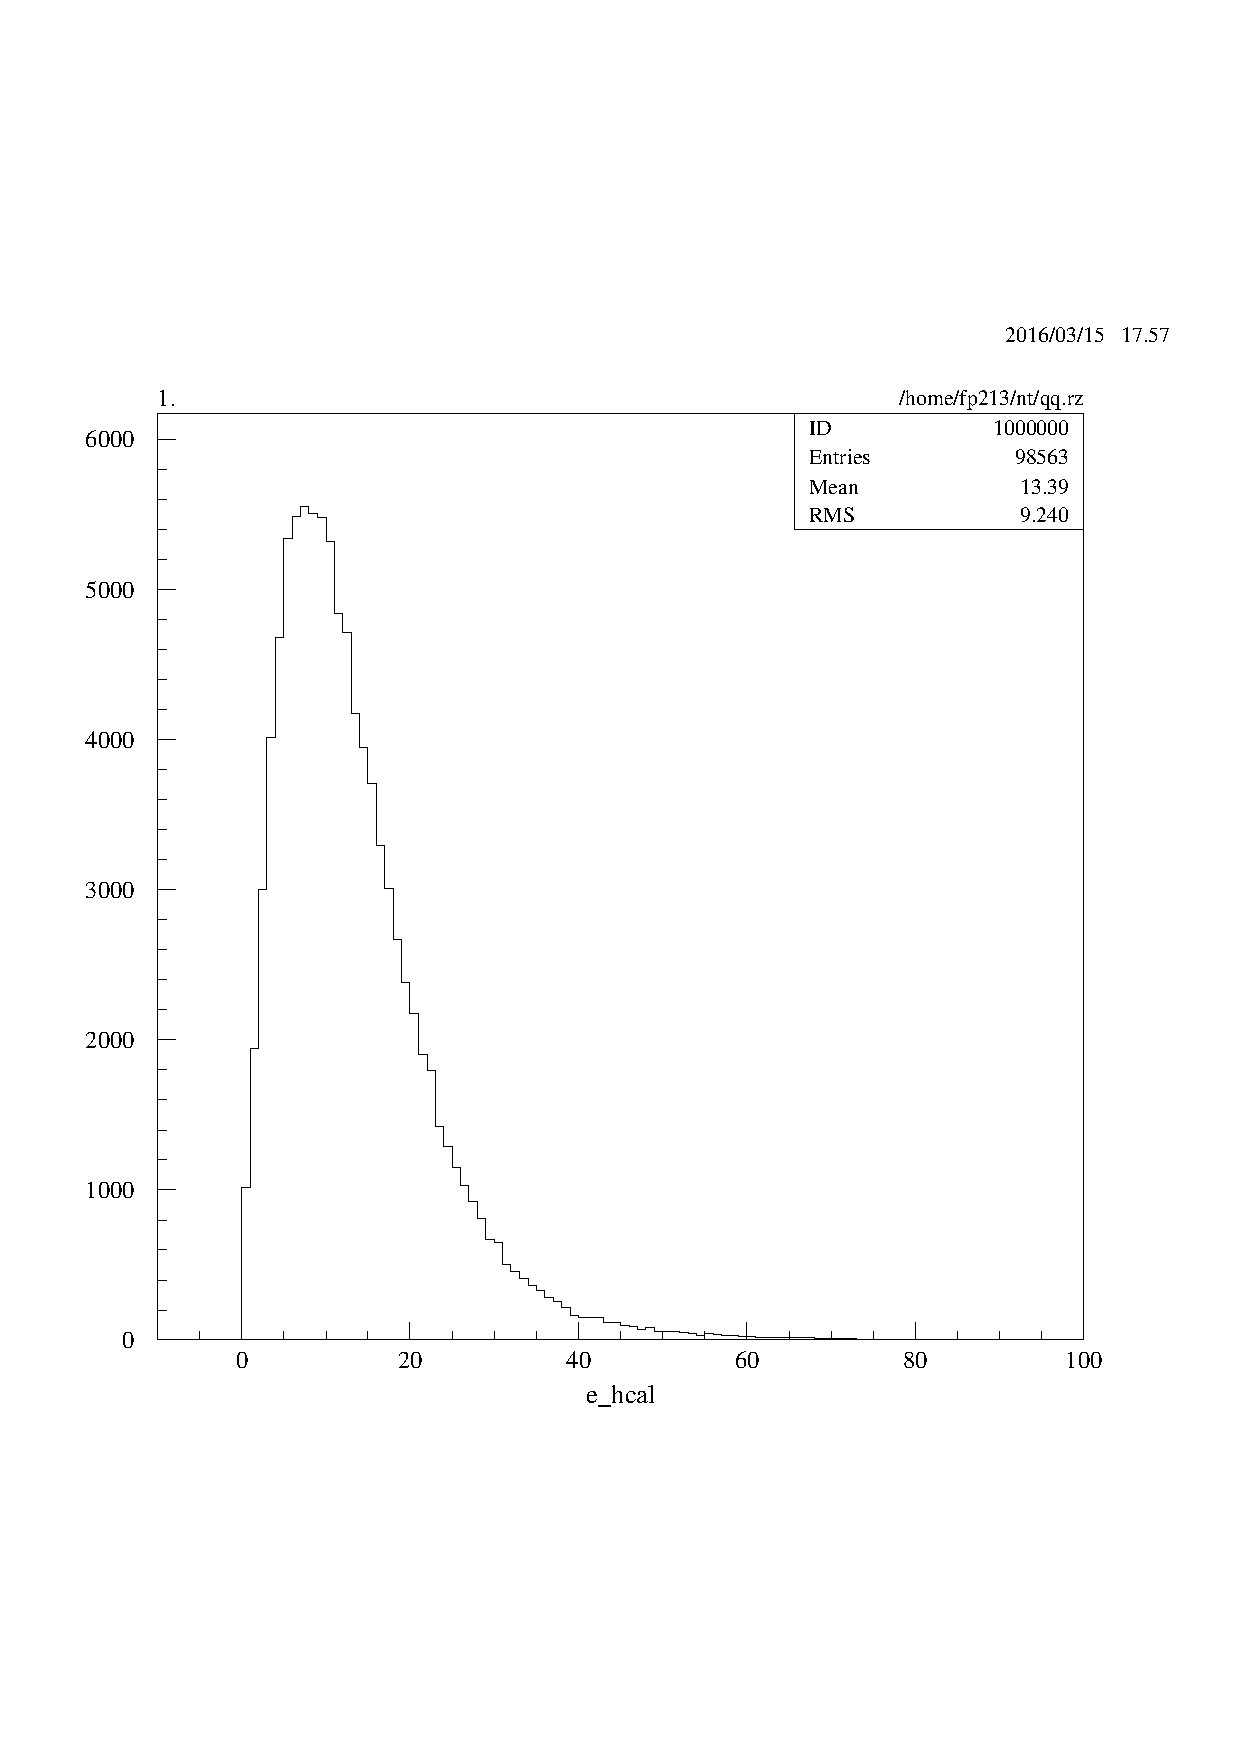
\includegraphics[width=\linewidth]{hadrons-e_hcal}
        \caption{%
            Hadrons
        }
        \label{fig:paw-e_hcal/hadrons}
    \end{subfigure}
    \caption{%
        Energy deposited into the \ehcal\ for the four decay types.
        Histograms generated with \textsc{paw} from Monte Carlo datasets.
    }
    \label{fig:paw-e_hcal}
\end{figure}

    
    \begin{figure}[h!]
    \centering
    \begin{subfigure}[c]{0.48\linewidth}
        \centering
        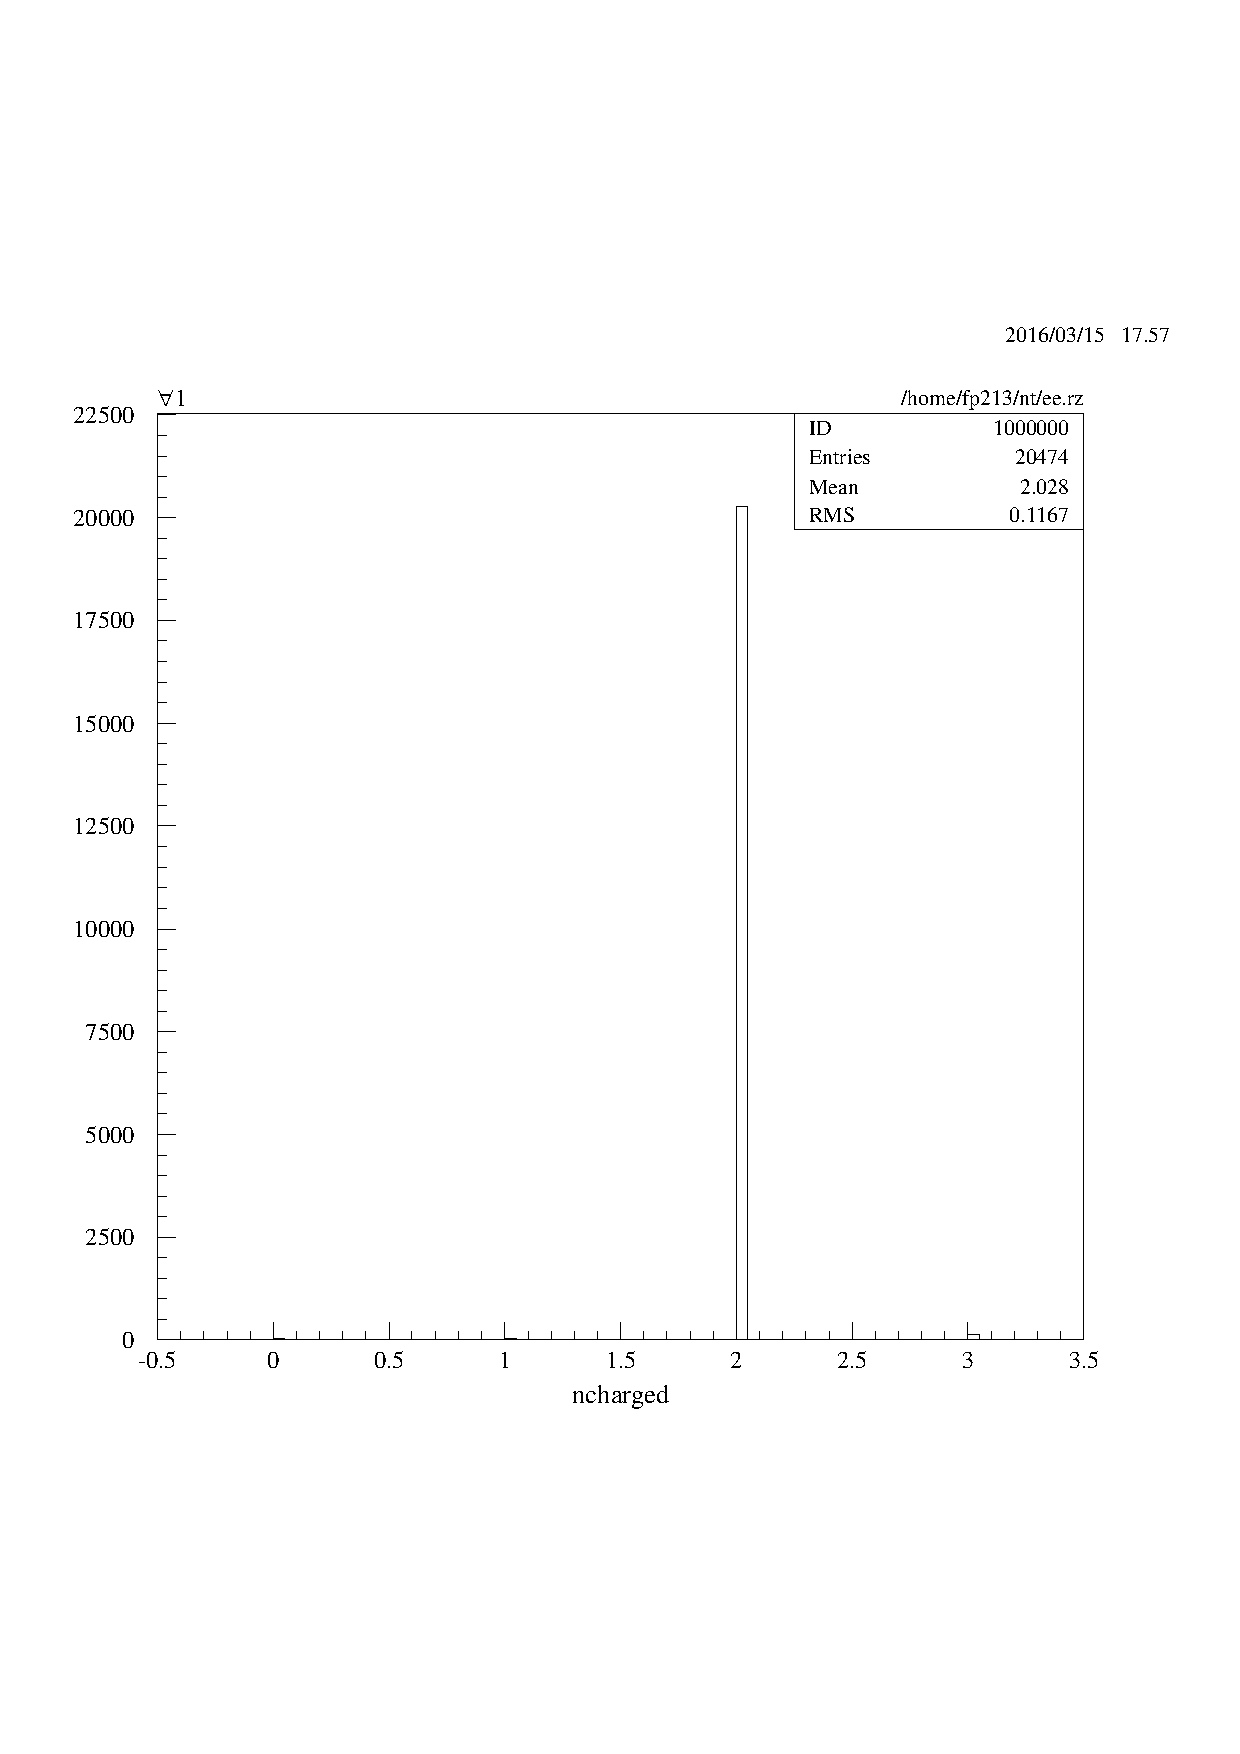
\includegraphics[width=\linewidth]{matrix-electrons-with-electron-filter}
        \caption{%
            Electrons with electron cut
        }
        \label{fig:paw-matrix/electrons}
    \end{subfigure}
    \hfill
    \begin{subfigure}[c]{0.48\linewidth}
        \centering
        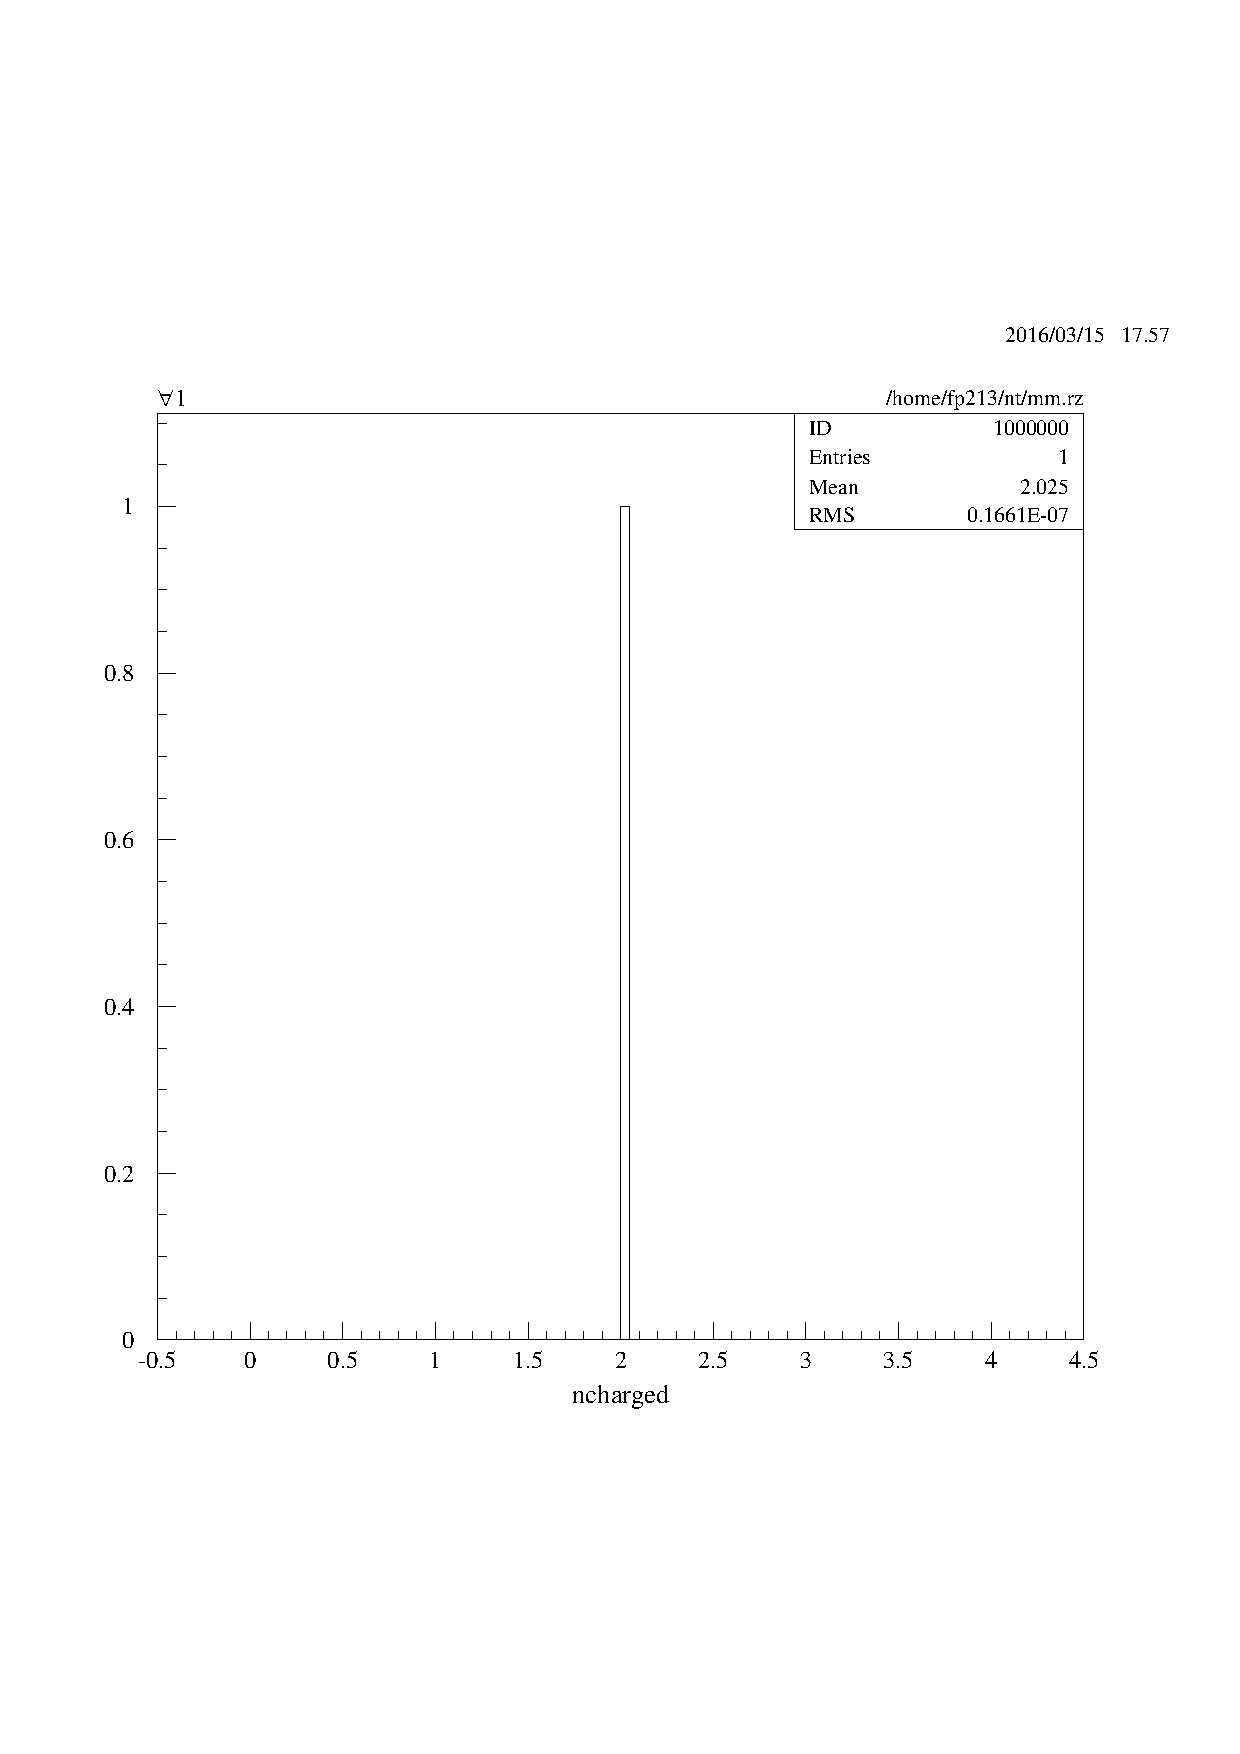
\includegraphics[width=\linewidth]{matrix-muons-with-electron-filter}
        \caption{%
            Muons with electron cut
        }
        \label{fig:paw-matrix/muons}
    \end{subfigure}
    \caption{%
        Histograms to obtain number of matched events in out cuts. Created with
        \textsc{paw} from Monte Carlo datasets.
    }
    \label{fig:paw-matrix-electrons}
\end{figure}


\end{appendix}

\end{document}

% vim: spell spelllang=en_us tw=79
